%%%%%%%%%%%%%%%%%%%%%%%%%%%%%%%%%%%%%%%%%%%%%%%%%%%%%%%%%%%%%%%%%%%%%%%%%%%%%%%%
% For the use of University of Amsterdam
% Master of AI thesis
%%%%%%%%%%%%%%%%%%%%%%%%%%%%%%%%%%%%%%%%%%%%%%%%%%%%%%%%%%%%%%%%%%%%%%%%%%%%%%%%

\documentclass[license]{mscaithesis}  % Can print or not a license
% The license is very optional and its definition easy to edit in mscaithesis.cls

\usepackage{mwe}  % Only for the example

\usepackage{amssymb} % Math packages are (on purpose) not included in the class document
\usepackage{amsfonts}
\usepackage{amsmath}
\usepackage{amsthm}

\usepackage{natbib}
\usepackage{booktabs} % nicer table rules
\usepackage{subcaption} % sub-figures (a)/(b)
\usepackage{tikz}
\usetikzlibrary{arrows.meta, positioning, fit, backgrounds}
\usepackage{pgfplots} % vector plots as code (no raster PNGs)
\pgfplotsset{compat=1.18}
\usepackage{listings} % verbatim prompts in the appendix
\lstset{basicstyle=\footnotesize\ttfamily, breaklines=true, breakindent=0pt,
  columns=fullflexible, keepspaces=true, frame=single, framesep=4pt,
  xleftmargin=3pt, aboveskip=4pt, belowskip=2pt}
\usepackage[most]{tcolorbox} % styled prompt boxes (appendix)
% teal box = vision-language model prompt; amber box = language model prompt
\newtcblisting{vlmprompt}[1]{breakable, enhanced, sharp corners,
  colframe=teal!55!black, colback=teal!4, coltitle=white,
  colbacktitle=teal!55!black, fonttitle=\bfseries\small, title={#1},
  listing only, listing options={basicstyle=\footnotesize\ttfamily,
  breaklines=true, breakindent=0pt, columns=fullflexible, keepspaces=true},
  boxrule=0.6pt, left=5pt, right=4pt, top=2pt, bottom=2pt}
\newtcblisting{llmprompt}[1]{breakable, enhanced, sharp corners,
  colframe=orange!75!black, colback=orange!6, coltitle=white,
  colbacktitle=orange!75!black, fonttitle=\bfseries\small, title={#1},
  listing only, listing options={basicstyle=\footnotesize\ttfamily,
  breaklines=true, breakindent=0pt, columns=fullflexible, keepspaces=true},
  boxrule=0.6pt, left=5pt, right=4pt, top=2pt, bottom=2pt}

% Reduce overfull lines in the narrow two-column layout: as a last resort, allow
% TeX to add up to 3em of extra stretch to hard-to-break lines rather than let
% text spill past the column edge.
\emergencystretch=3em

%%%%%%%%%%%%%%%%%%%%%%%%%%%%%%%%%%%%%%%%%%%%%%%%%%%%%%%%%%%%%%%%%%%%%%%%%%%%%%%%
% DOCUMENT METADATA
%%%%%%%%%%%%%%%%%%%%%%%%%%%%%%%%%%%%%%%%%%%%%%%%%%%%%%%%%%%%%%%%%%%%%%%%%%%%%%%%

% Thesis related entries
\title{RoboRef: A Foundation Reward Model for Robot Reinforcement Learning}
% \subtitle{A tale of computers}

% Date on which your thesis is submitted
\date{2026/07/17}

\author{Student \textsc{Platon Karageorgis}}
\studentnumber{15552055}
\period{2026/01/05 -- 2026/07/17}
\credits{36 ECTS}
\examiner{Pascal Mettes}
\dailysupervisor{Christian Gumbsch}
\uvasupervisor{Leonardo Barcellona, Stratis Gavves}  % Only if different from daily supervisor, leave empty otherwise
\addsupervisor{Rahaf Aljundi}  % Optional

\begin{document}
\maketitle

\frontmatter
        \chapter*{Abstract}
                \begin{adjustwidth}{4cm}{4cm}
                        Defining a reward is a long-standing problem in robot reinforcement learning (RL). Prior work has engineered complicated reward functions and heuristics, yet no single solution delivers both strong performance and generalization. The recent surge of vision-language models (VLMs), with impressive performance across domains, raises a key question: can state-of-the-art VLMs provide meaningful rewards and resolve the reward-definition bottleneck in robot RL? A handful of recent papers finetune state-of-the-art VLMs on large robotic datasets to investigate this question, with Robometer \citep{robometer} demonstrating the most competitive performance, yet the field remains largely unexplored. We introduce RoboRef, which builds on Robometer and introduces several innovations. First, we identify that its dataset lacks annotated failure trajectories conveying physical understanding, and re-curate it to fill this gap. Second, we incorporate in-context demonstrations to sharpen the model's notion of task success. Finally, because false positives mislead an optimizing policy far more than false negatives \citep{gumbsch_demonstrations_2026}, we propose an alternative loss that penalizes them to enforce conservatism. We evaluate RoboRef on offline metrics and downstream RL across three simulated benchmarks. We find that state-of-the-art reward models excel at offline reward metrics yet struggle as reward signals in downstream RL. RoboRef, in contrast, trains policies on tasks where the off-the-shelf baselines never learn at all and delivers the strongest overall downstream performance of any reward model we test, making it, to our knowledge, the state-of-the-art vision-language reward model.
                \end{adjustwidth}

\chapter*{Acknowledgements}
        \begin{adjustwidth}{4cm}{4cm}
                This thesis was made possible by the ELLIS Honours program, whose funding supported the work and opened the collaboration with Toyota Motor Europe (TME). I am grateful to my supervisors, Leonardo Barcellona, Rahaf Aljundi, Stratis Gavves, and Christian Gumbsch, for their guidance throughout the project, and to Pascal Mettes for examining this thesis. I want to add a special thank you to Christian for pushing me to my limits, helping me grow as a researcher, and supporting me with his positive mindset.
        \end{adjustwidth}

\tableofcontents

\listoffigures

\listoftables

\setlength{\parskip}{5pt}

\chapter{List of Symbols}
This list gathers the notation used throughout the thesis.

\subsection*{Inputs and trajectories}
\begin{tabular}{@{}p{1.9cm}p{6.0cm}p{1.9cm}p{6.0cm}@{}}
$l$ & task description given to the model & $T$ & frames per traj. ($8$ in Robometer, $16$ ours) \\
$t$ & frame index, $t=1,\dots,T$ & $o_t$ & $t$-th frame of the scored trajectory \\
$d_t$ & $t$-th frame of the demonstration & $o^1,o^2$ & the two trajectories of a preference pair \\
$h_t$ & hidden state at the $t$-th progress token & & \\
\end{tabular}

\subsection*{Labels and targets}
\begin{tabular}{@{}p{1.9cm}p{6.0cm}p{1.9cm}p{6.0cm}@{}}
$p_t$ & per-frame progress target, $p_t\in[0,1]$ & $s_t$ & per-frame success flag, $s_t\in\{0,1\}$ \\
$y$ & preference label for a pair & $s$ & rubric score, $s\in\{1,\dots,5\}$ \\
$p$ & normalized progress, $p=(s-1)/4$ & $y_t$ & ordinal rubric level of frame $t$ \\
\end{tabular}

\subsection*{Model outputs}
\begin{tabular}{@{}p{1.9cm}p{6.0cm}p{1.9cm}p{6.0cm}@{}}
$\hat{p}_t$ & predicted progress distribution over the bins & $\bar{p}_t$ & mean of $\hat{p}_t$, the scalar progress \\
$\hat{s}_t$ & predicted success probability & $\hat{y}$ & predicted preference probability \\
$N$ & number of progress bins, $N=10$ & $c_i$ & value of progress bin $i$ \\
$\mathrm{Proj}(\cdot)$ & projection of a scalar progress onto the bins & & \\
\end{tabular}

\subsection*{Objectives}
\begin{tabular}{@{}p{1.9cm}p{6.0cm}p{1.9cm}p{6.0cm}@{}}
$\mathcal{L}$ & total training loss & $\mathcal{L}_{\mathrm{prog}}$ & progress loss term \\
$\mathcal{L}_{\mathrm{succ}}$ & success loss term & $\mathcal{L}_{\mathrm{pref}}$ & preference loss term \\
$\lambda$ & asymmetry coefficient ($\lambda=0.3$) & $w_t$ & per-frame asymmetric weight (progress) \\
$\mathcal{N},\mathcal{P}$ & incomplete / complete frame sets & $k$ & ordinal threshold index, $k\in\{2,3,4,5\}$ \\
$z_{t,k}$ & CORN cumulative-threshold logits & $b_{t,k}$ & cumulative bit, $\mathbf{1}[y_t\ge k]$ \\
$\alpha_k$ & per-threshold weight, $1+c(k-2)$ & $c$ & CORN asymmetry hyperparameter ($c=1.5$) \\
$\lambda_{\mathrm{kl}}$ & weight of the KL anchor & $P_{\mathrm{old}},P_{\mathrm{new}}$ & stored / current progress distribution (KL anchor) \\
\end{tabular}

\subsection*{Other}
\begin{tabular}{@{}p{1.9cm}p{6.0cm}p{1.9cm}p{6.0cm}@{}}
$\sigma(\cdot)$ & logistic sigmoid & $d'$ & class separation, $(\mu_{\mathrm{succ}}-\mu_{\mathrm{fail}})/\sigma$ \\
$\tau$ & Kendall's rank correlation & & \\
$\langle\mathrm{prog}\rangle$ & per-frame progress marker token & $\langle\mathrm{pref}\rangle$ & preference token \\
$\langle\mathrm{split}\rangle$ & separator between two trajectories & $\langle\mathrm{demo\_end}\rangle$ & separator after the demonstration \\
\end{tabular}


\chapter{List of Abbreviations}
The following acronyms are used in the thesis.

\vspace{4pt}
\begin{tabular}{@{}p{1.8cm}p{6.1cm}p{1.8cm}p{6.1cm}@{}}
AI & Artificial intelligence & AUC & Area under the (ROC) curve \\
AUPRC & Area under the precision-recall curve & BCE & Binary cross-entropy \\
C51 & Categorical distributional value formulation & CE & Cross-entropy \\
CORN & Conditional ordinal regression for neural networks & DROID & Distributed robot interaction dataset \\
FPR & False positive rate & FSDP & Fully sharded data parallel \\
FT & Fine-tuned & GPU & Graphics processing unit \\
GVL & Generative value learning & IBRL & Imitation bootstrapped reinforcement learning \\
ICL & In-context learning & KL & Kullback-Leibler divergence \\
LLM & Large language model & LoRA & Low-rank adaptation \\
LRM & Large reward models & MLP & Multilayer perceptron \\
OOD & Out of distribution & PPO & Proximal policy optimization \\
RBM-1M & Robometer's 1M-trajectory dataset & RL & Reinforcement learning \\
RL-VLM-F & RL from vision-language model feedback & RLHF & RL from human feedback \\
ROC & Receiver operating characteristic & RQ & Research question \\
TPR & True positive rate & VLAC & Vision-language-action critic \\
VLM & Vision-language model & & \\
\end{tabular}



\twocolumn
\mainmatter
        \chapter{Introduction}
\label{sec:introduction}

% TODO(bibliography): citations below use \citep{} keys not yet in
% bibliographies/references.bib, so they render as [?] until the bibliography pass.
% Keys used here:
%   robodopamine -> RoboDopamine
%   roboreward   -> RoboReward
%   lrm          -> "Large Reward Models: Generalizable Online Robot Reward
%                    Generation with Vision-Language Models"
%   robometer    -> Robometer (Liang et al.)        [the base model we build on]
%   demo2reward  -> demo2reward (Gumbsch et al., 2026) [overconfidence claim]
%   brown2020    -> Brown et al., 2020, "Language Models are Few-Shot Learners"
%   dong2022     -> Dong et al., 2022, "A Survey on In-Context Learning"
% The Abstract still uses plain-text "(Liang et al.)"/"(Gumbsch et al., 2026)";
% convert both to \citep in the same pass.

Reinforcement learning (RL) offers a principled framework for teaching robots to act through trial and error, but it rests on a deceptively difficult prerequisite: a reward function that specifies what the robot should achieve. For robotic manipulation, designing this signal by hand is notoriously laborious and brittle. Dense, shaped rewards demand task-specific engineering and privileged state information --- object poses, contact flags, goal distances --- that is rarely available outside simulation, while sparse success rewards are easy to specify but hard to optimize. Worse, a reward crafted for one task seldom transfers to the next, so every new behavior reopens the same engineering problem. In practice the reward, rather than the policy optimizer, is often the true bottleneck: given a faithful reward the same RL loop learns readily, and without one it fails regardless of the algorithm.

Vision-language models (VLMs) trained on internet-scale data have recently shown broad visual and semantic understanding that transfers across domains with little or no task-specific tuning. This raises the prospect of a general, reusable reward: a model that simply watches an episode and judges whether --- and how much --- the task was accomplished, replacing per-task reward engineering with a single pretrained judge. It also poses the central question of this thesis: \textit{can state-of-the-art VLMs provide meaningful, generalizable rewards and resolve the reward-definition bottleneck in robot RL?}

Several recent works pursue this idea, training VLMs to predict rewards for robot behavior \citep{robodopamine, roboreward, lrm}. The most competitive of these is Robometer \citep{robometer}, a large multi-task VLM reward model trained on a corpus of over a million robot trajectories and equipped with dedicated output heads for success and task-progress prediction. Robometer reports strong offline reward-quality metrics, yet the field remains young and largely unexplored. In particular, these models are validated almost entirely by offline metrics computed on held-out clips; whether they actually function as reward signals inside a downstream RL loop --- the setting they are ultimately meant for --- has received far less scrutiny.

We introduce \textbf{RoboRef}, a VLM reward model that builds on Robometer through three contributions. The first, and most central, concerns the training data. Robometer supervises its two most important heads --- success and task progress --- almost exclusively on \emph{successful} trajectories; failures reach the model only indirectly, as the rejected side of a preference comparison. A reward model that has never been densely trained on failure has little reason to recognize it, yet recognizing failure is exactly what an RL policy will stress-test. We therefore drop the preference head and supervise the success and progress heads directly on failure trajectories. Doing so requires what, to our knowledge, does not yet exist: a robot dataset in which failed attempts carry \emph{dense, per-frame} progress annotations. Annotating failures densely is the crux of the problem. For a successful trajectory, progress can be approximated by how far the demonstration has advanced; a failed attempt has no such monotonic reference --- it may stall, regress, or briefly approach success before collapsing. We obtain reliable labels from two complementary sources. In simulation, we read the simulator's privileged state at every step, producing exact per-frame progress for a controlled spectrum of failure modes --- from an arm that never reaches the object, to a grasp that slips moments before completion. For real-world failures, where no such ground truth exists, we design a dual pipeline: a vision-language model first describes each frame in isolation, and a language model then acts as a judge that maps those descriptions to a per-frame progress score. Decoupling perception from adjudication in this way proved substantially more reliable than asking a single model to score an entire video.

Our second contribution introduces in-context demonstrations to the reward model. In-context learning --- supplying examples in the prompt so that a model adapts to a task without any weight update --- is among the defining capabilities of large pretrained models \citep{brown2020}, and has been shown to improve few-shot generalization across language and multimodal tasks \citep{dong2022}. For a reward model, a demonstration supplies precisely what a textual task description cannot: a concrete, visual definition of what success looks like for this embodiment, scene, and camera viewpoint. We pair each trajectory under evaluation with a successful demonstration of the same task and, to our knowledge, are the first to do so for a robot VLM reward model. This grounds the model's judgment in an example rather than in a potentially ambiguous instruction, sharpening its notion of task completion.

Our third contribution revisits the training objective. VLM reward models have been observed to be overconfident, systematically over-predicting success \citep{demo2reward}. In reinforcement learning, the two ways of being wrong are far from symmetric. A false positive --- the reward declaring success when the task has actually failed --- creates a spurious goal that an optimizing policy will actively seek out and exploit, the failure mode known as reward hacking. A false negative --- withholding reward from genuine success or progress --- is comparatively harmless: it can slow learning by making the reward signal sparser, but it never hands the policy a shortcut to exploit. A reward model used for RL should therefore err toward caution. We introduce a targeted, principled modification of the standard reward objective that penalizes over-prediction more heavily than under-prediction, biasing the model toward conservative, harder-to-exploit predictions.

We evaluate RoboRef both offline and as the reward signal for downstream RL, across two simulated manipulation benchmarks. Our experiments expose a sharp disconnect: reward models that excel on standard offline metrics can nonetheless fail completely as RL rewards, because an optimizing policy learns to exploit their false positives. RoboRef, by contrast, trains policies on tasks where the off-the-shelf baseline never learns at all, and outperforms prior reward models in both the offline and the downstream regime.

In summary, this thesis makes the following contributions:
\begin{itemize}
    \item \textbf{A failure-annotated reward dataset.} To our knowledge the first robot dataset with dense, per-frame progress labels on \emph{failure} trajectories, built from simulation ground truth and a dual VLM-then-LLM labeling pipeline.
    \item \textbf{In-context demonstrations for reward modeling.} A novel addition relative to prior VLM reward models, grounding the model's notion of task success in a concrete example rather than a text instruction.
    \item \textbf{An asymmetric reward objective.} A targeted modification of the standard loss that addresses the documented overconfidence of VLM reward models by penalizing false positives, yielding more conservative and less exploitable rewards.
\end{itemize}
Along the way, we surface an observation with implications beyond our own model: the offline metrics reported by current VLM reward models do not predict their usefulness as downstream RL rewards --- a gap we examine directly.

These contributions and observations are organized around the following \textit{preliminary} research questions. Our main research question is:

\noindent\textit{To what extent can a fine-tuned vision-language model serve as a usable and generalizable reward signal for downstream robot reinforcement learning?}

\noindent which we approach through four sub-questions:
\begin{itemize}
    \item \textbf{RQ1.} Does supervising the reward model on curated failure trajectories with dense per-frame progress labels improve its ability to discriminate success from failure?
    \item \textbf{RQ2.} Are VLM reward models overconfident, and does an asymmetric loss that penalizes false positives yield more conservative, less exploitable rewards?
    \item \textbf{RQ3.} Do offline reward-quality metrics predict downstream RL performance?
    \item \textbf{RQ4.} Under what conditions can a fine-tuned VLM reward model train a policy where state-of-the-art baselines fail?
\end{itemize}

        \chapter{Related Work}
\label{sec:related-work}

Our work belongs in an interdisciplinary area. We learn a reward instead of designing one, we follow the recent wave of vision-language reward models for robots, we prioritize the use of failure data, we borrow in-context learning techniques, and we draw on the study of reward hacking. We review each in turn and say where RoboRef departs from it.

\section{Learned rewards for reinforcement learning}

Reinforcement learning needs a reward, and a long line of work tries to obtain that reward from data instead of writing it by hand. Inverse reinforcement learning recovers a reward function from expert demonstrations \citep{ng_algorithms_2000, abbeel_apprenticeship_2004}, while reward shaping adds guidance to a sparse reward without changing which policy is optimal \citep{ng_policy_1999}. A second strand drops the need for demonstrations and learns from human preferences over pairs of trajectory segments \citep{christiano_deep_2017}, an idea that later aligned large language models through reinforcement learning from human feedback \citep{ouyang_training_2022}. Most recently, foundation models have themselves become the source of feedback. RL-VLM-F, for instance, asks a VLM which of two images better satisfies a task and trains a reward from its answers \citep{wang_rl-vlm-f_2024}. 

Across all of these, the reward is no longer hand-written but learned, which is the setting we work in. Learning the reward brings a risk that a carefully designed reward does not. A learned reward can be wrong in structured, repeatable ways, and a policy that optimizes against it can find and exploit those mistakes. We return to this risk in Section~\ref{sec:reward-hacking}, since it is central to why our objective is built the way it is.

\section{Vision-language reward models for robotics}
\label{sec:related-vlm}

The most direct precursors to our work are VLMs trained specifically to score robot behavior. They take a video of a robot attempting a task together with a language description, and they return a reward that estimates its progress. They differ in what exactly they output, in how they use failure data, and in whether and how they are tested as an actual reward inside reinforcement learning. Table~\ref{tab:vlm-reward-models} summarizes the most prominent ones.

\begin{table*}[t]
\centering
\footnotesize
\caption[Vision-language reward models compared]{Vision-language reward models for robot manipulation. The last column reports whether the model was tested as the reward inside an RL loop, in which domain, and whether the tested reward was the released model used without in-domain adaptation.}
\label{tab:vlm-reward-models}
\begin{tabular}{@{}p{2.0cm}p{1.9cm}p{2.3cm}p{2.9cm}p{2.0cm}p{3.2cm}@{}}
\toprule
Model & Backbone & Training data & Reward output & Failure data & Downstream RL \\
\midrule
Robometer \citep{robometer} & Qwen3-VL-4B & $>$1M trajectories, 21 embodiments & dense per-frame progress and success, plus a comparison head & yes, through trajectory comparisons & real-world (zero-shot); simulation only with an in-domain LoRA variant \\
\addlinespace
RoboReward \citep{roboreward} & Qwen3-VL, 4B and 8B & $\sim$54k examples (Open X, RoboArena) & a single discrete 1--5 score for the whole episode &synthetic, from clipped or relabeled successes & real-world, zero-shot; simulation only as a baseline-VLM reward-type study \\
\addlinespace
Robo-Dopamine \citep{robodopamine} & RoboBrain 2.0 (Qwen2.5-VL), 3B and 8B & $\sim$100k trajectories, 3.4k hours of video & dense signed progress; needs a goal image and multi-view & no, expert successes only & simulation and real, after one-shot in-domain adaptation \\
\addlinespace
Large Reward Models \citep{TRI-reward-model} & Qwen3-VL-8B (LoRA) & multi-source, total size not reported & dense progress, a completion flag, and a contrastive term & indirect, via temporal ordering & simulation, zero-shot online (PPO); real-world via offline self-improvement \\
\bottomrule
\end{tabular}
\end{table*}

Robometer \citep{robometer} is the model we build on, and we describe it in Chapter~\ref{sec:robometer}. It predicts dense per-frame progress and success and learns from failure data through trajectory comparisons. RoboReward \citep{roboreward} instead returns a discrete score from one to five for the whole episode, and it builds the negatives it needs by clipping successful videos short or relabeling them across tasks, so its failures are artifacts of editing, not genuine failed attempts. Robo-Dopamine \citep{robodopamine} produces a dense, signed progress signal, but it requires a goal image and multiple camera views as inputs, and it trains on expert successes instead of failures. Large Reward Models \citep{TRI-reward-model} combine a dense progress estimate with a binary completion flag and a contrastive term learned from the temporal order of frames. One recent model sits outside our table because it is not built on a VLM. The World Value Model \citep{wang_world_2026} breaks from the shared assumption of the others by building its value estimator on a pretrained video world model, and not a VLM, on the argument that the temporal priors of a world model suit progress estimation better than the static-image representations behind VLMs. It predicts dense per-frame progress and, closest to our own concerns, targets suboptimal execution directly, introducing a small-scale benchmark of human-labeled suboptimal trajectories with dense per-frame values.

Two patterns in Table~\ref{tab:vlm-reward-models} matter for this thesis. The first is that not every model is tested in downstream RL with its final, released reward. Robometer's only simulated RL run uses a variant fine-tuned in-domain on LIBERO and not the released model. RoboReward tests its trained model in the real world only. Robo-Dopamine adapts its reward to each task from a single demonstration before learning. Large Reward Models is the clean case, driving simulated reinforcement learning zero-shot with its trained, frozen model. Yet even in this case, the analysis behind the RL performance remains shallow. A foundation reward model should justify its training cost with strong results in simulated and real-world RL alike, in-distribution and out of distribution (OOD). These models instead report headline success rates without examining the offline-to-online gap or the reward exploitation we find at its center. The second pattern is failure. Only some of these models train on failure data at all, and none assembles a large training corpus of genuine failed attempts with dense, per-frame progress labels, which is the gap our dataset fills. World Value Model is the closest, but its dense labels form a small, human-annotated evaluation benchmark, not a training set at scale.

A number of related reward and value models share our motivation without being direct points of comparison. VLAC \citep{zhai_vision-language-action-critic_2025} predicts a dense progress delta and a done signal for real-world RL, and transfers to new tasks from a single in-context example. GVL \citep{ma_vision_2025} casts value estimation as ordering shuffled frames and reads values out of a vision-language model in context, with no training at all. ReWiND \citep{zhang_rewind_2025} learns a language-conditioned reward from a small set of demonstrations and then adapts to unseen tasks with little further interaction. Together these show how much can be done with a frozen or lightly trained foundation model, but none of them confronts the failure-labeling and reward-exploitation problems that we focus on.

\section{Learning from failure data}

Most reward and policy learning for robots leans on expert or successful data, and failure, when it is used at all, is treated as something to detect, not something to measure progress within. This is beginning to change. RoboFAC builds a large dataset of erroneous trajectories with question-answer annotations and uses it to analyze and correct robot failures \citep{lu_robofac_2025}, and FailSafe generates failure cases together with recovery actions so that vision-language-action models can notice and undo their mistakes \citep{lin_failsafe_2025}. Generalist robot policies have begun to use failure directly as well. $\pi_{0.7}$ trains on large amounts of suboptimal and failed robot data and conditions the policy on mistake labels that humans annotate by hand, so that it can be steered away from those mistakes at test time \citep{pi07_2026}. These efforts show that a failure carries information a success does not. Failure data is scarce and expensive to label, though, which is why most reward models avoid it.

Our use of failure is different. We do not label failures in order to detect or recover from them. We give them dense, per-frame progress, so the same heads that score a success learn what partial and aborted progress looks like, and a model queried on an OOD scene where the robot has drifted off the task, knocking over an object mid-grasp for instance, can still flag the failure. To our knowledge no existing robot dataset provides this at training scale.

\section{In-context learning}

In-context learning is the ability of a large pretrained model to perform a task from examples placed in its input, without any change to its weights \citep{brown_language_2020}. While it has become one of the most studied properties for improving few-shot generalization across language and general multimodal tasks \citep{dong_survey_2024, wang_qwen2-vl_2024}, its application in embodied AI and robotics is still emerging. Most robotic applications of in-context learning focus on policy generation or high-level planning; its use inside robot reward models remains unexplored.

The closest examples in the reward modeling space either avoid training or avoid visual grounding. GVL reads values out of a vision-language model conditioned on in-context information, but it does so entirely zero-shot without any training \citep{ma_vision_2025}. Conversely, Demo2Reward optimizes the language instruction of a reward model at test time by using demonstrations, but focuses on textual prompt tuning instead of visual in-context learning \citep{gumbsch_demonstrations_2026}. Neither approach trains a foundation reward model to natively process visual demonstrations as part of its evaluative forward pass.

We bring in-context learning directly into the training loop of a robot reward model, so that a single model serves both modes, scoring a trajectory on its own or next to a successful demonstration of the same task. When a demonstration is present, the model no longer depends on the task description alone; the example shows it what success looks like in that scene and embodiment. As far as we can tell, no earlier robot reward model has trained with demonstrations in the loop this way.

\section{Reward hacking in reward models}
\label{sec:reward-hacking}

Because a learned reward function serves as a surrogate objective for the true underlying task, optimizing a policy strictly against this proxy often introduces objective misalignment. The phenomenon where an agent exploits flaws in a learned reward function was identified early as a critical safety challenge \citep{amodei_concrete_2016}. It has since been extensively documented in reinforcement learning from human feedback (RLHF) for language models, where optimizing a policy beyond a certain threshold degrades actual performance even as the proxy reward score continues to climb \citep{gao_scaling_2023}. This vulnerability is equally pervasive in robotic manipulation; a policy can actively find and exploit states that the reward model mistakenly scores as successful.

This issue is particularly acute for a reward driving reinforcement learning, where a false positive misleads an optimizing policy far more than a false negative \citep{gumbsch_demonstrations_2026}. This observation directly motivates our asymmetric training objective, which explicitly penalizes over-prediction more severely than under-prediction, and it anticipates our broader finding that strong offline validation does not guarantee a reward stays robust under online policy optimization.
        \chapter{Robometer}
\label{sec:robometer}

This thesis builds directly on Robometer \citep{robometer}, so before turning to our own method we describe how it works in detail. In its own evaluation Robometer outperforms almost every prior vision-language reward model, which is why we build on it, the one exception being \citet{TRI-reward-model}, published a few weeks later. Our contributions change specific parts of this design, the data it learns from, the heads it trains, and the loss it minimizes, so the goal of this chapter is to introduce the baseline architecture and training objective to the reader. We cover the backbone it is built on and how it turns a video and an instruction into per-frame predictions, the three heads it carries and the objective that trains them, how those predictions serve as a reward, how progress and success are labeled, how clips become training samples, how it learns from comparisons, and the data it learns from. Figure~\ref{fig:robometer-overview} gives the model at a glance.

\begin{figure*}[t]
\centering
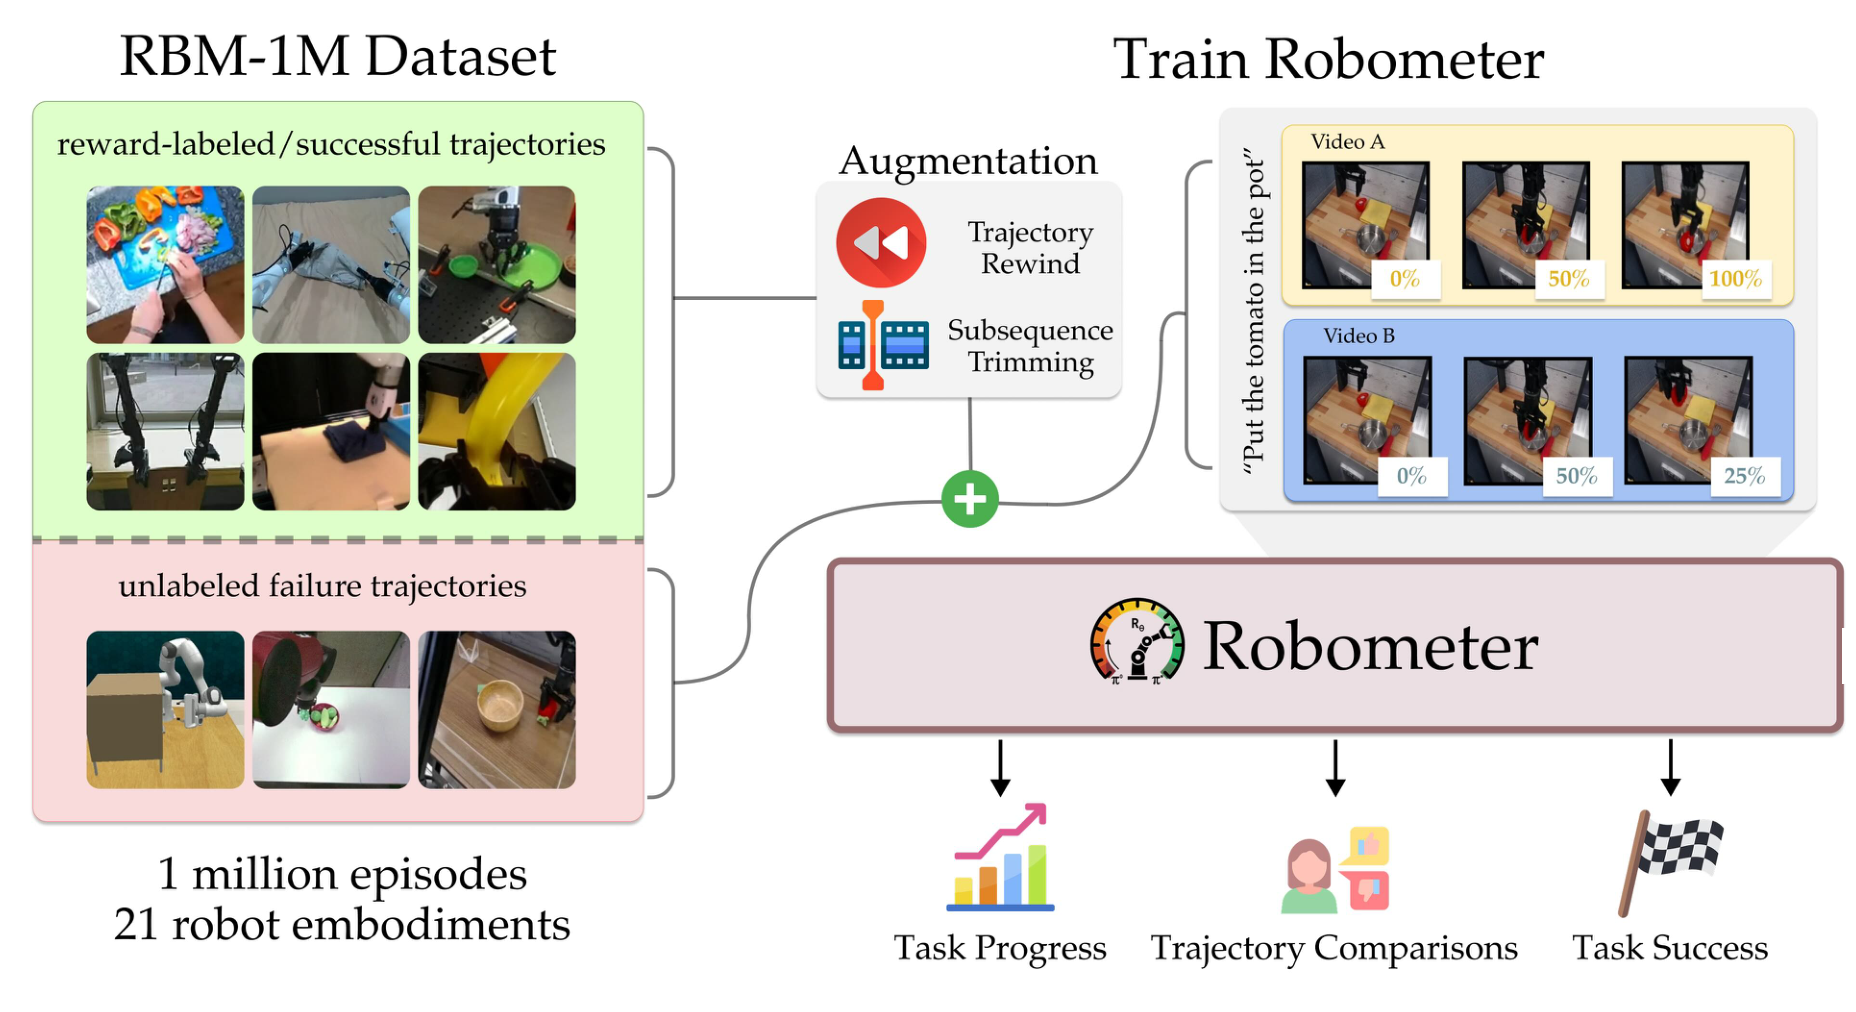
\includegraphics[width=0.85\textwidth]{media/robometer_overview.png}
\caption[Overview of Robometer]{An overview of Robometer, the reward model this thesis builds on, adapted from \citet{robometer}. Robometer is trained on RBM-1M, which pairs reward-labeled successful trajectories with unlabeled failures. During training these clips are augmented by trajectory rewind and subsequence trimming (Section~\ref{sec:bg-sampling}), and the model is supervised on three outputs, per-frame task progress, per-frame task success, and trajectory comparisons, which are the three heads this chapter describes.}
\label{fig:robometer-overview}
\end{figure*}

\section{Inputs and backbone}

Robometer is built on Qwen3-VL-4B-Instruct \citep{team_qwen3-vl_2025}, a pretrained vision-language model. Such a model has already learned, from large-scale image and text data, to recognize objects, read scenes, and connect them to language, and this prior knowledge is what lets a reward model generalize to tasks and robots it was not explicitly trained on. Robometer keeps this backbone and adapts it to scoring robot task videos.

A trajectory is presented as a short sequence of $T$ frames $o_1, \dots, o_T$ (with $T = 8$ in the paper's configuration) sampled evenly from the video, together with the task description $l$. To produce a prediction at each individual frame, Robometer inserts a learned progress token $\langle\mathrm{prog}\rangle$ directly after each frame. Writing $\mathrm{Tok}(\cdot)$ for the tokens an input produces, which for a video already carry the backbone's own video-start delimiter, the model sees
\begin{equation}
\mathrm{Tok}(l)\;\big[\,\mathrm{Tok}(o_t)\,\langle\mathrm{prog}\rangle\,\big]_{t=1}^{T} .
\label{eq:input-single}
\end{equation}
Robometer is also trained by comparison, learning which of two attempts at the same task is the better one, a preference-learning signal we return to in Section~\ref{sec:bg-comparisons}. This comparison uses a second input layout, in which two trajectories of the same task, $o^1$ and $o^2$, are placed one after the other, separated by a split token, with a single preference token $\langle\mathrm{pref}\rangle$ appended at the very end,
\begin{multline}
\mathrm{Tok}(l)\;\big[\,\mathrm{Tok}(o^1_t)\,\langle\mathrm{prog}\rangle\,\big]_{t=1}^{T}\;\langle\mathrm{split}\rangle\\
\big[\,\mathrm{Tok}(o^2_t)\,\big]_{t=1}^{T}\;\langle\mathrm{pref}\rangle .
\label{eq:input-pair}
\end{multline}
The state at this final preference token is what the model reads to decide which of the two trajectories, the first or the second, is the better attempt.

The backbone is causally masked, and this is what lets the model read every per-frame prediction from a single forward pass. In the single-trajectory input of Equation~\ref{eq:input-single}, the hidden state at the $t$-th progress token, which we write $h_t$, is the vector the backbone's final transformer layer outputs at that token's position, a single embedding of the model's hidden dimension. Because of the causal mask it can attend only to the instruction and to frames $1$ through $t$, so it is a running summary of the trajectory up to frame $t$. In the paired input of Equation~\ref{eq:input-pair}, the preference token sits after both trajectories and attends to all of them. The hidden states at these tokens, and nothing else, are what the prediction heads read.

\section{Three prediction heads}

Robometer attaches three lightweight heads on top of the shared backbone, each answering a different question.

\begin{itemize}
    \item \textbf{Progress.} For every frame, how far the task has advanced, on a scale from zero, meaning nothing has been accomplished, to one, meaning the task is complete. This is the dense, per-step signal that a policy can follow.
    \item \textbf{Success.} For every frame, whether the task has actually been completed, expressed as a probability. This is a standard binary reward that answers yes or no, instead of describing the percentage of the task that is complete.
    \item \textbf{Trajectory comparison.} Given two trajectories for the same task, which of the two is better. This head does not score a single trajectory in isolation. It orders a pair.
\end{itemize}

Each head is a small two-layer MLP applied to a progress or preference token's hidden state, and the three are trained together under a single objective,
\begin{equation}
\mathcal{L} = \mathcal{L}_{\mathrm{prog}} + \mathcal{L}_{\mathrm{succ}} + \mathcal{L}_{\mathrm{pref}} ,
\label{eq:total-loss}
\end{equation}
one term per head. We describe each head together with the loss that trains it. The per-frame targets these losses compare against, $p_t$, $s_t$, and $y$, are defined later in the chapter.

The \emph{success} head maps each progress-token state $h_t$ to a single logit, $\hat{s}_t = \sigma(\mathrm{MLP}_{\mathrm{succ}}(h_t)) \in [0,1]$, the probability that the task is complete at frame $t$. It is trained with a class-balanced binary cross-entropy against the binary target $s_t$,
\begin{equation}
\mathcal{L}_{\mathrm{succ}} = \frac{1}{T}\sum_{t=1}^{T} \mathrm{BCE}\!\big(s_t,\, \hat{s}_t\big).
\end{equation}

The \emph{progress} head is where Robometer departs from a plain regressor. Instead of predicting a single number, $\mathrm{MLP}_{\mathrm{prog}}(h_t)$ produces $N = 10$ logits, one for each of a fixed set of progress values, or bins, spaced evenly across $[0,1]$, following the C51 distributional formulation \citep{bellemare2017c51}. A softmax turns these logits into a distribution $\hat{p}_t \in \Delta^{N}$ over the bins, and a scalar progress value is read back as its expectation $\sum_{i=1}^{N} \hat{p}_{t,i}\, c_i$, where $c_i$ is the value of bin $i$. Modeling progress as a distribution, not a point estimate makes the target smoother to fit and lets the model express uncertainty about how far along it is. The head is trained with a cross-entropy between this distribution and the target progress encoded onto the same bins,
\begin{equation}
\mathcal{L}_{\mathrm{prog}} = \frac{1}{T}\sum_{t=1}^{T} \mathrm{CE}\!\big(\mathrm{Proj}(p_t),\, \hat{p}_t\big).
\end{equation}
The projection operator $\mathrm{Proj}(p_t)$ encodes the continuous ground-truth progress $p_t \in [0,1]$ into a target distribution over the $N$ bins. For $N=10$ the bins sit at $0.0, 0.11, 0.22, \dots, 1.0$, and since a true progress value rarely lands exactly on one, $\mathrm{Proj}$ splits a total mass of $1$ between the two closest bins, weighted by proximity. 

Consider a ground-truth progress of $p_t = 0.27$. It falls between the third bin ($0.22$) and the fourth ($0.33$), and since it is closer to $0.22$, the lower bin takes the larger share of the mass ($57\%$) and the upper bin the rest ($43\%$), chosen so that the mean of the target distribution reconstructs $p_t = 0.27$ exactly.

The \emph{preference} head maps the single preference-token state to one logit, $\hat{y} = \sigma(\mathrm{MLP}_{\mathrm{pref}}(h_{\langle\mathrm{pref}\rangle}))$, the probability that the first trajectory is the better of the pair. It is trained with a binary cross-entropy against the label $y \in \{0,1\}$ that marks which trajectory is better,
\begin{equation}
\mathcal{L}_{\mathrm{pref}} = -\big[\, y\log\hat{y} + (1-y)\log(1-\hat{y}) \,\big].
\label{eq:pref-loss}
\end{equation}

The success and progress heads produce the reward for a single trajectory and are the only ones used at deployment. The preference head needs a pair of trajectories, so it cannot score a lone trajectory and plays no role once the model is deployed; it exists only to shape training, in the way we make precise in Section~\ref{sec:bg-comparisons}, which is also why we do not include it in our own model.

\section{Using Robometer as a reward}

At deployment, Robometer takes a single trajectory and its task description and runs one forward pass. For each frame $t$ it reads the progress-token hidden state $h_t$ and passes it through the two task heads, which produce one success logit and $N = 10$ progress logits. A sigmoid on the success logit gives the per-frame success probability $\hat{s}_t$, and a softmax over the progress logits gives the per-frame progress distribution $\hat{p}_t$, whose mean is the scalar progress. The output of the model is therefore, for every frame, a success probability and a progress value.

A downstream reinforcement learning algorithm calls the model in place of a hand-designed or simulator reward and uses one of these per-frame quantities, the progress value or the success probability, as the reward signal. Because each frame's prediction depends only on the frames before it, the model can score a trajectory online as it grows, returning a reward at every step and not only at the end, which is what makes it usable inside a reinforcement learning loop.

The targets these heads are trained against, $p_t$ and $s_t$ for the two task heads and $y$ for the preference head, are where Robometer's design becomes consequential for our work, and we turn to how they are built next.

\section{How progress and success are labeled}

The progress head needs a dense per-frame target, and the success head a per-frame binary flag. Robometer obtains both cheaply for successful demonstrations by assuming that an expert demonstration advances steadily toward the goal. A demonstration of length $T$ is labeled by setting the progress target $p_t = t/T$, so it rises evenly from zero at the first frame to one at the last, while the success target $s_t$ is a binary flag, zero until the task is finished and one from completion onward. A frame one second into a two-second task is therefore marked half done. No human annotation is needed, because a successful demonstration reaches the goal by construction. There is one practical detail to note. A recording often keeps rolling for a moment after the task is already finished, so its final frames show no real progress. Robometer handles this by marking progress as complete slightly before the last frame, at a cutoff point chosen separately for each dataset.

As a concrete example, take a clip of a robot placing a cup on a shelf (Figure~\ref{fig:cup-labels}). The progress target climbs from zero as the arm reaches and lifts the cup, passes roughly one half as it carries the cup across, and reaches one as the cup settles on the shelf. The success target, by contrast, stays at zero for the entire approach and flips to one only at the moment the cup is in place.

\begin{figure*}[h]
\centering
% MetaWorld shelf-place success inst0000, eight of sixteen keyframes; progress = t/T.
\begin{tikzpicture}
\begin{axis}[scale only axis, width=0.944\textwidth, height=2.6cm,
  xmin=0.5, xmax=8.5, xtick=\empty, ymin=0, ymax=1.15, ytick={0,0.5,1},
  ylabel={Target}, axis lines=left, ymajorgrids, grid style={gray!18},
  tick label style={font=\scriptsize}, label style={font=\footnotesize},
  legend style={font=\scriptsize, at={(0.015,0.74)}, anchor=north west, draw=none, fill=none},
  legend cell align=left, enlarge x limits=false, clip=false]
\addplot[thick, mark=*, mark size=1.5pt, color=blue!65!black]
  coordinates {(1,0)(2,0.13)(3,0.27)(4,0.4)(5,0.6)(6,0.73)(7,0.87)(8,1)};
\addlegendentry{progress $p_t = t/T$}
\addplot[thick, dashed, color=orange!88!black]
  coordinates {(1,0)(6.5,0)(6.5,1)(8,1)};
\addlegendentry{success $s_t$}
\node[anchor=south, inner sep=0, yshift=2pt] at (axis cs:1,1.15) {
\includegraphics[width=0.118\textwidth]{media/sim/shelf_success/f0.jpg}};
\node[anchor=south, inner sep=0, yshift=2pt] at (axis cs:2,1.15) {
\includegraphics[width=0.118\textwidth]{media/sim/shelf_success/f1.jpg}};
\node[anchor=south, inner sep=0, yshift=2pt] at (axis cs:3,1.15) {
\includegraphics[width=0.118\textwidth]{media/sim/shelf_success/f2.jpg}};
\node[anchor=south, inner sep=0, yshift=2pt] at (axis cs:4,1.15) {
\includegraphics[width=0.118\textwidth]{media/sim/shelf_success/f3.jpg}};
\node[anchor=south, inner sep=0, yshift=2pt] at (axis cs:5,1.15) {
\includegraphics[width=0.118\textwidth]{media/sim/shelf_success/f4.jpg}};
\node[anchor=south, inner sep=0, yshift=2pt] at (axis cs:6,1.15) {
\includegraphics[width=0.118\textwidth]{media/sim/shelf_success/f5.jpg}};
\node[anchor=south, inner sep=0, yshift=2pt] at (axis cs:7,1.15) {
\includegraphics[width=0.118\textwidth]{media/sim/shelf_success/f6.jpg}};
\node[anchor=south, inner sep=0, yshift=2pt] at (axis cs:8,1.15) {
\includegraphics[width=0.118\textwidth]{media/sim/shelf_success/f7.jpg}};
\end{axis}
\end{tikzpicture}
\caption[Progress and success targets on a success clip]{The two training targets on a successful clip, a MetaWorld shelf-place episode that stands in for the cup example. Eight of sixteen keyframes are shown. Beneath them the progress target rises linearly with $t/T$ as the arm reaches, grasps, lifts, and places the block, while the success target stays at zero until the block is on the shelf and then jumps to one. A successful demonstration is labeled this way for free, with no annotation.}
\label{fig:cup-labels}
\end{figure*}

The same assumption fails for failures. A failed attempt does not advance evenly toward completion. It may stall at the start, move in the wrong direction, or come close to success and then fall apart, so a label like $t/T$ no longer reflects what is actually happening. Producing trustworthy per-frame progress labels for failures is therefore genuinely difficult, and Robometer sidesteps the difficulty by not labeling failures densely at all. This single decision is the starting point for our own work.

\section{From clips to training samples}
\label{sec:bg-sampling}

One more piece of Robometer's training recipe matters for what follows. The model is not trained on whole clips. Each training sample is a window cut from a stored trajectory, with boundaries drawn at random, and the frames inside the window receive fresh targets when the sample is built. On top of this windowing, Robometer generates progress samples through four strategies, drawn with equal probability. A \emph{forward} sample plays a window in its natural order, so its targets rise. A \emph{reverse} sample traverses the window backward, so its targets fall, teaching the model that progress can be undone. A \emph{rewind} sample runs forward and then back again, placing a regression in the middle of an otherwise normal clip; the authors ablate this strategy and find that removing it hurts failure detection. A \emph{different-task} sample keeps the frames but swaps in the instruction of another task and sets every progress target to zero, grounding the score in the instruction and not in motion alone. Our fine-tunes in Chapter~\ref{sec:methodology} inherit this sampling machinery unchanged, and it applies to our dense failure labels exactly as it does to the $t/T$ ramps, with the window's labels drawn from the stored per-frame values.

A second detail sits inside the same machinery. The success target is not labeled independently of progress. It is derived from it, with a frame marked complete exactly when its progress target reaches the completion cutoff described above. The two heads therefore share one labeling pipeline, and anything that shapes the progress targets shapes the success targets with it.

\section{Learning from comparisons}
\label{sec:bg-comparisons}

We now return to the third head, the preference head, and to the loss $\mathcal{L}_{\mathrm{pref}}$ of Equation~\ref{eq:pref-loss} that trains it. This head is what lets Robometer still benefit from the large pool of non-expert and failed trajectories, even without dense labels for them, and it does so through comparison, in the spirit of preference-based reward learning \citep{wang_rl-vlm-f_2024}. Given two trajectories of the same task, it sets the preference label $y = 1$ when the first is the better of the two and $y = 0$ otherwise, and trains the head to predict it through $\mathcal{L}_{\mathrm{pref}}$. A comparison needs only the relative ordering of the pair, not an exact value for either side, so it scales naturally to unlabeled and failed data, where a failed attempt simply becomes the lower-ranked side against an expert success.

The authors further report that comparisons help even when both trajectories succeed. Ranking a complete demonstration above a suboptimal but still successful one, for instance, gives the model an ordering signal that sharpens the progress and success heads without any failure data at all.

The consequence matters for this thesis. The progress and success heads learn almost entirely from successful trajectories, where the $t/T$ labels exist. Failed attempts reach the model only indirectly, as the lower-ranked side of a comparison. In other words, the two heads that actually generate the reward at deployment never see failure as a direct training target.

\section{Training data}

Robometer is trained on a corpus the authors call RBM-1M, roughly one million trajectories spanning twenty-one robot embodiments. It is drawn from public robot datasets, human videos, and simulation. Expert robot demonstrations form the largest single part, but a substantial share of the corpus comes from human video and from humanoid-robot data, which pushes its visual and embodiment coverage well beyond standard manipulator arms. We give a fuller breakdown of this corpus in Appendix~\ref{apx:rbm1m}, and of the changes we make to it in Appendix~\ref{apx:roboref-data}.

        \chapter{RoboRef}
\label{sec:methodology}

% Citation keys used here (verify against Zotero): robometer, roboreward,
%   yu_meta-world_2019, mclean_meta-world_2025, lin_failsafe_2025.
% ManiSkill is named but not cited; add a key if we want one.

This chapter describes RoboRef. We keep Robometer's backbone and its per-frame design, analyzed in Chapter~\ref{sec:robometer}, and we change three things: the data the model learns from, the way it reads a demonstration alongside the trajectory it has to score, and the loss it minimizes. We describe the dataset first, because both the changes to the model and the experiments depend on it. We then turn to the in-context demonstrations, the asymmetric objective, and how we train the model variants we compare. The protocol we use to evaluate the resulting models, both offline and as a reward for downstream reinforcement learning, is presented alongside the results in Chapter~\ref{sec:results}.

\section{A failure-annotated dataset}
\label{sec:method-dataset}

Chapter~\ref{sec:robometer} established the gap we start from. Robometer trains its two deployment heads, progress and success, only on successful trajectories, where assuming that an expert advances steadily toward the goal hands each frame a target for free. Failed attempts reach the model only through the preference head, as the lower-ranked side of a comparison, so neither deployment head ever sees failure as a direct target. The two heads are not equally hard to fix. The success head needs only a per-frame binary flag, and for a failed attempt that flag is simply zero at every frame, since the task is never completed. The progress head is the difficult one. It needs a dense progress value at every frame, and for a failure that value does not follow from the frame index, because a failed attempt does not advance steadily. What is missing is therefore a corpus whose failures carry dense per-frame progress, and to our knowledge no such corpus exists. We build one by re-curating and expanding RBM-1M, the corpus behind Robometer.

\subsection{Re-curating RBM-1M}

We make five changes to the corpus.

\begin{itemize}
    \item We hold the humanoid and human-only data out of the main training corpus. RBM-1M draws a large share of its size from humanoid robots and from human videos, which broaden its visual coverage but sit far from the single-arm manipulation our downstream tasks involve. Keeping them out of the shared corpus sharpens it around the embodiments we focus on. However, we do not discard them completely. We keep a smaller sample and use it in our model ablations (Section~\ref{sec:method-training}), where their extra visual coverage feeds the pretraining of one variant.
    \item We replace Robometer's FailSafe split with our own. FailSafe \citep{lin_failsafe_2025} is a simulated set of contact-rich cube tasks, lifting, pushing, and stacking a block on a tabletop. We discard their version and generate a fresh set of FailSafe failures in simulation, labeled densely (Section~\ref{sec:method-sim-failures}).
    \item RoboReward \citep{roboreward} released a dataset alongside its reward model, and RBM-1M incorporates a portion of it. We replace this RoboReward split with our own. It supplies two kinds of failure data, semantically wrong executions produced by counterfactual instruction relabeling (e.g. \textit{pick up the kettle} becomes \textit{pick up the spoon}), and genuine partial executions that stop before the task is finished. We discard the whole original split and draw a smaller sample of the partial executions alone, labeled by their own clip scores. Section~\ref{sec:method-roboreward} explains the replacement and the labeling.
    \item We add DROID \citep{khazatsky_droid_2024} failures. DROID is a large real-world dataset of a robot arm performing everyday tabletop manipulation across many scenes and tasks. Robometer uses DROID for successful demonstrations only; we add failed attempts, and alongside them a small set of successful DROID clips from the same tasks and camera setups. Keeping matching successes is deliberate. Our in-context training (Section~\ref{sec:method-icl}) pairs every trajectory with a successful demonstration of the same task, so each pool of added failures needs same-task successes to draw those demonstrations from. We follow the same rule for the other failure sources we add.
    \item We add MetaWorld \citep{yu_meta-world_2019, mclean_meta-world_2025} data, mostly failures, generated from scratch in simulation (Section~\ref{sec:method-sim-failures}). MetaWorld is a simulated benchmark of a single robot arm across 46 tabletop manipulation tasks, from reaching and pushing to pick-and-place and operating buttons and drawers. RBM-1M already carried a small MetaWorld set, the 100 demonstrations from ReWiND \citep{zhang_rewind_2025}, which we drop in favor of our own.
\end{itemize}

Table~\ref{tab:roboref-dataset} reports the resulting mix. The single-arm corpus that every model shares holds $648{,}714$ rows, of which $116{,}786$ are failures and $531{,}928$ are successes. The bulk of the successes are the standard-arm expert demonstrations we retain from RBM-1M; the failures come from the four sources we add or replace plus the Robometer failures we keep and label for the first time. The humanoid and human-only pool sits apart from this. It adds a further $214{,}427$ successful trajectories, used only in the Qwen3.5 pretraining phase and shown as a separate block at the foot of the table, which brings the full corpus to $863{,}141$ rows. Appendix~\ref{apx:rbm1m} gives the full composition of RBM-1M itself, Appendix~\ref{apx:roboref-data} expands Table~\ref{tab:roboref-dataset} to one row per upstream source together with the labeling, pairing, and sampling details, and Appendix~\ref{apx:gallery} lists the simulated task families and their failure modes in full.

\begin{table*}[t]
\centering
\footnotesize
\caption[Composition of the RoboRef dataset]{Composition of the RoboRef dataset. A row is one scored video clip, that is, one episode rendered from one camera view. \emph{Provenance} states whether a source is retained from RBM-1M, replaced with our own version, or newly added. \emph{Failure labels} names where the dense per-frame failure labels come from; successful trajectories everywhere use Robometer's $t/T$ heuristic. The block at the foot holds the humanoid and human-only data, which every model leaves out of shared training and only the Qwen3.5 model sees, in its first phase alone. Counts are not directly comparable to Robometer's Table~IX, which reports unique video-language annotations expanded across views.}
\label{tab:roboref-dataset}
\begin{tabular}{@{}p{4.6cm}p{1.8cm}p{2.4cm}rrr@{}}
\toprule
Source & Provenance & Failure labels & Failures & Successes & Total \\
\midrule
Robometer expert demonstrations & retained & --- & 0 & 490{,}798 & 490{,}798 \\
Robometer mixed-expertise archives & retained & VLM+LLM & 68{,}923 & 26{,}029 & 94{,}952 \\
\addlinespace
MetaWorld (ours) & added & simulator physics & 24{,}402 & 1{,}850 & 26{,}252 \\
FailSafe (ours) & replaced & simulator physics & 2{,}098 & 75 & 2{,}173 \\
DROID (ours) & added & VLM+LLM & 5{,}503 & 5{,}863 & 11{,}366 \\
RoboReward (ours) & replaced & ramp to clip score & 15{,}860 & 7{,}313 & 23{,}173 \\
\midrule
Standard-arm total & & & 116{,}786 & 531{,}928 & 648{,}714 \\
\midrule
\multicolumn{6}{@{}l}{\emph{Held out of shared training; used only for the Qwen3.5 first phase}}\\
Humanoid & retained & --- & 0 & 112{,}629 & 112{,}629 \\
Human-only & retained & --- & 0 & 101{,}798 & 101{,}798 \\
\midrule
Total with phase-1 data & & & 116{,}786 & 746{,}355 & 863{,}141 \\
\bottomrule
\end{tabular}
\end{table*}

\subsection{Labeling failures densely}

A successful demonstration is almost free to label. As we explained in previous chapters, if a clip has $T$ frames and the expert reaches the goal at the end, we set the progress at frame $t$ to $t/T$, a value that climbs evenly from zero at the first frame to one at the last. A failure has no such reference. It may stall, drift away from the task, or briefly approach success and then fall apart, so its progress does not climb steadily and cannot be read off the frame index. Which route we take to label a failure depends on its dataset family. 

For the failures we generate ourselves in simulation, MetaWorld and FailSafe, we have the simulator's true state and read progress straight from it (Section~\ref{sec:method-sim-failures}). For the rest of the failures where we only possess a recorded video, we infer progress from the frames with a two-stage model pipeline (Section~\ref{sec:method-real-failures}). This video-only group is larger than it first appears. It covers the real-world failure clips already in RBM-1M and the DROID failures we add. It also contains some simulated data already in RBM-1M from other dataset families, such as RACER \citep{dai_racer_2025} evaluated in RLBench \citep{james_rlbench_2020}, whose videos we keep but whose simulator we never run due to time constraints. The RoboReward partial executions are a third, unique, case (Section~\ref{sec:method-roboreward}). Since they are shortened clips of actual demonstrations, they are monotone by construction. Thus, they are labeled by the simple ramp that successes used, described above. So, they need neither of the two routes.

Whatever the route, every failure label lands on one common scale. Each failure frame first gets a rubric score $s \in \{1,2,3,4,5\}$, which we map to a normalized progress value $p = (s-1)/4$, so the five levels become $\{0, 0.25, 0.5, 0.75, 1.0\}$. A genuine failure never completes the task, so its scores stay in $\{1,2,3,4\}$ and its progress never reaches $1.0$.

However, this format is different from the one that successes use, as these per-frame scores would give a failure a stair-step target, flat within a level and jumping at each change of level, whereas a success target is the smooth $t/T$ ramp. We do not want the model to tell failures from successes by the shape of the target alone, a staircase against a ramp, so we smooth the failure target. When a training sample is built, we interpolate each failure's progress linearly between the frames where its level changes, which turns the staircase into a ramp that still passes through the rubric values. Failures and successes then share one continuous target on $[0,1]$, the scale the progress head predicts over, and the successes keep their $t/T$ labels untouched. 

One could in principle relabel the successes with the same two-stage pipeline we use for the video failures (Section~\ref{sec:method-real-failures}) to remove this asymmetry, but its language-model stage is expensive and the success corpus is far too large for that to be practical, so the successes stay on the cheap $t/T$ heuristic. Furthermore, someone could argue that the pure monotonicity of the success data could discriminate between success and failure data. Thus, in preliminary experiments described in Chapter~\ref{sec:results} we also tried to add noise to success labels and break their pattern; however, it proved suboptimal in our experiments.

This normalized progress value $p$ is then encoded for the progress head exactly as described in Chapter~\ref{sec:robometer}. The value is projected into a discrete target distribution over $N=10$ bins, and the progress head is trained using a cross-entropy loss between this target and its own prediction. Simultaneously, the success head is trained on a binary completion flag, which remains strictly zero at every frame of a failed trajectory.

\subsection{Simulated failures}
\begin{figure*}[t]
\centering
% Frames are simulator renders (raster); the label curve below is PGFPlots (code).
% FailSafe stack carry_drop inst0002, eight of sixteen keyframes; labels 1 1 2 3 3 3 1 1.
\begin{subfigure}{\textwidth}
\centering
\begin{tikzpicture}
% frames live inside the axis (axis cs) so they sit exactly above the curve points
\begin{axis}[scale only axis, width=0.944\textwidth, height=2.4cm,
  xmin=0.5, xmax=8.5, xtick=\empty, ymin=0.7, ymax=4.3, ytick={1,2,3,4},
  ylabel={Score}, axis lines=left, ymajorgrids, grid style={gray!18},
  tick label style={font=\scriptsize}, label style={font=\footnotesize},
  enlarge x limits=false, clip=false]
\addplot[thick, mark=*, mark size=1.5pt, color=blue!65!black]
  coordinates {(1,1)(2,1)(3,2)(4,3)(5,3)(6,3)(7,1)(8,1)};
\node[anchor=south, inner sep=0, yshift=2pt] at (axis cs:1,4.3) {
\includegraphics[width=0.118\textwidth]{media/sim/failsafe/f0.jpg}};
\node[anchor=south, inner sep=0, yshift=2pt] at (axis cs:2,4.3) {
\includegraphics[width=0.118\textwidth]{media/sim/failsafe/f1.jpg}};
\node[anchor=south, inner sep=0, yshift=2pt] at (axis cs:3,4.3) {
\includegraphics[width=0.118\textwidth]{media/sim/failsafe/f2.jpg}};
\node[anchor=south, inner sep=0, yshift=2pt] at (axis cs:4,4.3) {
\includegraphics[width=0.118\textwidth]{media/sim/failsafe/f3.jpg}};
\node[anchor=south, inner sep=0, yshift=2pt] at (axis cs:5,4.3) {
\includegraphics[width=0.118\textwidth]{media/sim/failsafe/f4.jpg}};
\node[anchor=south, inner sep=0, yshift=2pt] at (axis cs:6,4.3) {
\includegraphics[width=0.118\textwidth]{media/sim/failsafe/f5.jpg}};
\node[anchor=south, inner sep=0, yshift=2pt] at (axis cs:7,4.3) {
\includegraphics[width=0.118\textwidth]{media/sim/failsafe/f6.jpg}};
\node[anchor=south, inner sep=0, yshift=2pt] at (axis cs:8,4.3) {
\includegraphics[width=0.118\textwidth]{media/sim/failsafe/f7.jpg}};
\end{axis}
\end{tikzpicture}
\caption[FailSafe stack, dropped]{FailSafe stack: a cube grasped and carried, then dropped to the table. The score climbs to $3$ and falls back to $1$.}
\end{subfigure}

\vspace{5pt}

% MetaWorld pick-place late_drop inst0005, eight of sixteen keyframes; labels 1 1 2 3 4 3 3 3.
\begin{subfigure}{\textwidth}
\centering
\begin{tikzpicture}
\begin{axis}[scale only axis, width=0.944\textwidth, height=2.4cm,
  xmin=0.5, xmax=8.5, xtick=\empty, ymin=0.7, ymax=4.3, ytick={1,2,3,4},
  ylabel={Score}, axis lines=left, ymajorgrids, grid style={gray!18},
  tick label style={font=\scriptsize}, label style={font=\footnotesize},
  enlarge x limits=false, clip=false]
\addplot[thick, mark=*, mark size=1.5pt, color=blue!65!black]
  coordinates {(1,1)(2,1)(3,2)(4,3)(5,4)(6,3)(7,3)(8,3)};
\node[anchor=south, inner sep=0, yshift=2pt] at (axis cs:1,4.3) {
\includegraphics[width=0.118\textwidth]{media/sim/metaworld/f0.jpg}};
\node[anchor=south, inner sep=0, yshift=2pt] at (axis cs:2,4.3) {
\includegraphics[width=0.118\textwidth]{media/sim/metaworld/f1.jpg}};
\node[anchor=south, inner sep=0, yshift=2pt] at (axis cs:3,4.3) {
\includegraphics[width=0.118\textwidth]{media/sim/metaworld/f2.jpg}};
\node[anchor=south, inner sep=0, yshift=2pt] at (axis cs:4,4.3) {
\includegraphics[width=0.118\textwidth]{media/sim/metaworld/f3.jpg}};
\node[anchor=south, inner sep=0, yshift=2pt] at (axis cs:5,4.3) {
\includegraphics[width=0.118\textwidth]{media/sim/metaworld/f4.jpg}};
\node[anchor=south, inner sep=0, yshift=2pt] at (axis cs:6,4.3) {
\includegraphics[width=0.118\textwidth]{media/sim/metaworld/f5.jpg}};
\node[anchor=south, inner sep=0, yshift=2pt] at (axis cs:7,4.3) {
\includegraphics[width=0.118\textwidth]{media/sim/metaworld/f6.jpg}};
\node[anchor=south, inner sep=0, yshift=2pt] at (axis cs:8,4.3) {
\includegraphics[width=0.118\textwidth]{media/sim/metaworld/f7.jpg}};
\end{axis}
\end{tikzpicture}
\caption[MetaWorld pick-place, dropped]{MetaWorld \texttt{pick-place}: the puck lifted toward the goal, then dropped. The score reaches $4$ and falls back to $3$.}
\end{subfigure}

\caption[Dense non-monotonic failure labels from simulation]{Dense, non-monotonic failure labels from simulation. Each strip shows eight keyframes of a failed attempt, and the curve beneath plots the per-frame progress score read directly from the simulator state. In both cases the score rises as the arm makes progress and then regresses when the object is dropped. These plotted scores are the ground-truth training targets.}
\label{fig:sim-failures}
\end{figure*}

\label{sec:method-sim-failures}

In simulation we do not collect failures and then label them. We choose a target rubric score and attempt to generate a failure whose progress lands on it. For a task and a target score, the pipeline runs a scripted expert until a pre-defined signal, a progress measure such as the gripper-to-object distance or the grasp flag, crosses a task-specific injection point. Once that happens, it switches to a noise mode that induces a particular kind of failure and runs on for only a short, fixed number of steps before we end the episode. The MetaWorld pick-place episode in Figure~\ref{fig:sim-failures} is one such near-success failure. The scripted expert lifts the puck and carries it almost to the goal, and only there does the noise controller force the gripper open, so the puck drops and the attempt fails just short. Keeping this post-injection phase short is deliberate. If the robot flailed under noise for a long time, the sixteen frames we later subsample would be dominated by that phase and leave too few for the clean run-up before the failure. The injection point fixes how far the attempt gets before it breaks. For a target of one the noise starts at once, for two once the arm has reached the object, for three once the object is grasped and moved, and for four only deep into the task. We keep an episode only if the simulator's state-based detector confirms it ended at the intended score, then subsample it uniformly to sixteen frames.

The noise modes are specific to each simulator. MetaWorld uses nine. They are \emph{random} (fully random actions), \emph{wrong-direction} (a strong bias away from the goal), \emph{freeze} (the arm holding position with a fraction of the expert's force), \emph{drop} (the gripper forced open mid-transport), \emph{late-drop} (the gripper forced open just short of the goal, Figure~\ref{fig:sim-failures} bottom), \emph{misplace} (the expert action plus a small offset near the goal), \emph{lift-away} (the arm lifting off and losing contact), \emph{push-sideways} (the arm pushing perpendicular to the goal), and \emph{partial-actuation} (the expert driving a mechanism or button most of the way and then stalling short of completion). Which modes apply depends on the task family and the target score. A grasping task reaches its near-complete failures through \emph{drop} and \emph{late-drop}, a pushing task through \emph{lift-away} and \emph{push-sideways}, and a mechanism or button through \emph{partial-actuation}, while \emph{random}, \emph{wrong-direction}, and \emph{freeze} cover the low scores everywhere. Appendix~\ref{apx:gallery} gives the full task-and-mode breakdown. FailSafe builds its three cube tasks from the analogous behaviors: moving away from the cube, freezing before contact, approaching and then retreating, grasping and then freezing, carrying without releasing, dropping mid-carry (Figure~\ref{fig:sim-failures} top), and, near the goal, releasing or nudging the cube just short of success. A handful of runs complete the task for an instant and are then disturbed, so the cube is knocked back out of place.

Because the simulator exposes the true state at every step, the per-frame progress comes straight from physics, with no model in the loop. This gives us the property we care about most. The label tracks the behavior, and it falls when the behavior regresses. When the arm drops a grasped object the progress steps back down, and when a briefly completed task is disturbed it falls from the top of the scale. A monotone $t/T$ label cannot represent this backward motion, and it is exactly what we want the progress head to learn to read.

We generate two such sets. MetaWorld \citep{yu_meta-world_2019, mclean_meta-world_2025} gives a simulated Sawyer robot arm over 46 manipulation tasks, with failures at every pre-success score. We hold a subset of the tasks out of training and reserve them for evaluation, so no task seen at test time appears during training. FailSafe, built in the ManiSkill simulator \citep{mu_maniskill_2021, tao_maniskill3_2024}, gives the three contact-rich cube tasks above, where the hardest cases reach a near-success score before failing. Every episode is rendered from three camera viewpoints, and because the labels come from physics and not pixels they are identical across the three views.


\subsection{Real-world failures}
\begin{figure*}[t]
\centering
% Per-frame (unrolled) view. Frames are raster DROID renders; everything else is TikZ.
% Frames, descriptions, and scores are real outputs. Prompts are in the appendix.
\resizebox{\textwidth}{!}{%
\begin{tikzpicture}[
  font=\footnotesize, >={Latex[length=2.2mm]},
  frame/.style={draw=gray!45, inner sep=1pt, rounded corners=1pt},
  desc/.style ={draw=teal!55!black, fill=teal!8, rounded corners=3pt, align=left,
                inner sep=4pt, text width=5.0cm, font=\scriptsize},
  grade/.style={draw=orange!80!black, fill=orange!16, rounded corners=3pt, align=center,
                inner sep=4pt, text width=1.7cm, font=\footnotesize},
  tlab/.style ={font=\scriptsize\itshape, text=gray!45!black},
  outtag/.style={font=\scriptsize\itshape},
  ell/.style={font=\large\bfseries, text=gray!55!black},
]
% task header
\node[anchor=west, font=\footnotesize] (hdr) at (-5.6,3.9)
  {\textbf{Task:} ``Stack 3 cups.''\quad\textcolor{gray!55!black}{8 frames sampled; three shown}};
% left stage labels (horizontal), with model names and explicit outputs
\node[anchor=east, align=left, text width=2.6cm, font=\scriptsize, text=teal!40!black] (st1) at (-2.95,-0.25)
  {\textbf{Stage 1\,---\,describe}\\[1pt]{\ttfamily\scriptsize Qwen3.5-VL-35B-A3B}\\[1pt]reads each frame on its own.\\[2pt]\emph{Output: one description per frame.}};
\node[anchor=east, align=left, text width=2.6cm, font=\scriptsize, text=orange!55!black] (st2) at (-2.95,-5.05)
  {\textbf{Stage 2\,---\,grade}\\[1pt]{\ttfamily\scriptsize Qwen3-32B}\\[1pt]reads each description with all earlier ones.\\[2pt]\emph{Output: a 1--4 score per frame.}};
% frame index labels (above the frames)
\node[tlab] (tl1) at (0,2.85)    {frame 2};
\node[tlab] (tl2) at (5.9,2.85)  {frame 7};
\node[tlab] (tl3) at (11.8,2.85) {frame 8};
% frames + ellipses (8 frames sampled; three shown)
\node[frame] (f1) at (0,1.5)    {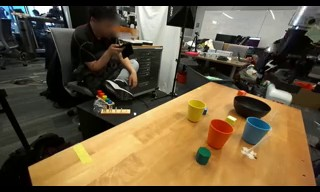
\includegraphics[width=3.8cm]{media/pipeline/cups1.jpg}};
\node[frame] (f2) at (5.9,1.5)  {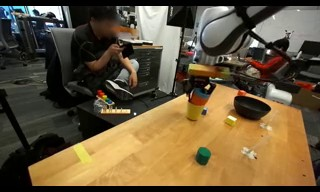
\includegraphics[width=3.8cm]{media/pipeline/cups2.jpg}};
\node[frame] (f3) at (11.8,1.5) {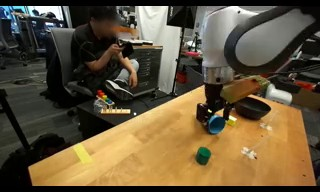
\includegraphics[width=3.8cm]{media/pipeline/cups3.jpg}};
\node[ell] at (2.95,1.5) {$\cdots$};
% descriptions (real, condensed) -- VLM output
\node[outtag, text=teal!45!black, anchor=west] at (-2.5,-0.95) {VLM output};
\node[desc] (d1) at (0,-2.0)
  {\textbf{Objects:} three cups on the table. \textbf{Gripper:} empty, above the table. \textbf{Progress:} no cups stacked yet.};
\node[desc] (d2) at (5.9,-2.0)
  {\textbf{Objects:} the cups, now stacked. \textbf{Gripper:} on the top cup. \textbf{Progress:} the stack is briefly complete.};
\node[desc] (d3) at (11.8,-2.0)
  {\textbf{Objects:} the cups, scattered on the table again. \textbf{Gripper:} empty. \textbf{Progress:} the stack has toppled; the attempt fails.};
% grade cells -- LLM output
\node[outtag, text=orange!55!black, anchor=west] at (-2.5,-4.35) {LLM output};
\node[grade] (L1) at (0,-5.05)    {{\scriptsize score}\\[1pt]{\large\textbf{1}}};
\node[grade] (L2) at (5.9,-5.05)  {{\scriptsize score}\\[1pt]{\large\textbf{4}}};
\node[grade] (L3) at (11.8,-5.05) {{\scriptsize score}\\[1pt]{\large\textbf{1}}};
% arrows
\draw[->,teal!60!black,thick] (f1) -- (d1);
\draw[->,teal!60!black,thick] (f2) -- (d2);
\draw[->,teal!60!black,thick] (f3) -- (d3);
\draw[->,thick] (d1) -- (L1);
\draw[->,thick] (d2) -- (L2);
\draw[->,thick] (d3) -- (L3);
\draw[->,orange!80!black,thick] (L1) -- node[above=1pt,font=\scriptsize,text=orange!55!black]{$+$ earlier descriptions} (L2);
\draw[->,orange!80!black,thick] (L2) -- node[above=1pt,font=\scriptsize,text=orange!55!black]{$+$ earlier descriptions} (L3);
% stage bands + outer container
\begin{scope}[on background layer]
  \node[fill=teal!5,   rounded corners=4pt, fit=(st1)(tl1)(tl3)(f1)(f3)(d1)(d3), inner sep=8pt] (b1){};
  \node[fill=orange!5, rounded corners=4pt, fit=(st2)(L1)(L3),         inner sep=8pt] (b2){};
  \node[draw=gray!45, line width=0.8pt, rounded corners=6pt, fit=(hdr)(b1)(b2), inner sep=6pt] {};
\end{scope}
\end{tikzpicture}%
}
\caption[The two-stage labeling pipeline]{Our two-stage labeling pipeline for real-world failures, unrolled over three of the eight sampled frames of one DROID episode, depicting a failed attempt to stack three cups. In the first stage a vision--language model (Qwen3.5-VL-35B-A3B) describes each frame on its own. In the second stage a language model (Qwen3-32B) grades each frame on the one-to-four failure rubric (five is not allowed to avoid hallucinations), reading the current description together with all earlier ones, which the horizontal arrows carry. The score climbs to four once the cups are stacked, then falls back when the stack topples. Stacking three cups is a multi-step task, so the language model first decomposes it into ordered sub-steps and grades against them. The detailed prompts can be found in Appendix~\ref{apx:prompts}. The frames, descriptions, and scores shown are real outputs.}
\label{fig:vlm-llm-pipeline}
\end{figure*}

\label{sec:method-real-failures}

For the failures where we have access only to the video of their trajectory, we infer the label from the frames, using two models in sequence. The first is a vision-language model, Qwen3.5-VL-35B-A3B. It looks at each frame on its own, independently of the others, and answers three fixed questions:
\begin{enumerate}
    \item which task-relevant objects are present and in what state
    \item what the gripper is doing at that moment
    \item what has been accomplished so far, measured against the goal.
\end{enumerate}
It sees one frame at a time, together with the task description, and answers in a few short sentences. Figure~\ref{fig:vlm-llm-pipeline} traces one clip through both stages, and the full prompt is in Appendix~\ref{apx:prompts}.

The second model is a language model, Qwen3-32B, which never sees the images. It reads the frame descriptions in the order they occur and assigns each one a progress score. The grading is cumulative. To score frame $t$ the model is given the descriptions of frames $1$ through $t$ along with the score it gave the previous frame, and it may lower a score only when the descriptions show that progress was genuinely undone.

The rubric it grades against has five levels, and a failure can reach only the first four. They are similar to the ones described in the simulation setup. A score of one is no meaningful progress, the arm never engaging the object the task is about. Two is contact without commitment, the object approached or touched but taken no further. Three is real partial progress, at least one sub-goal met, typically the object grasped and carried toward its target. Four is a near miss, the attempt carried almost to the end and broken only at the last moment, a grasp that slips or a placement that just fails to land. Five would mean the task is complete, which no clip in this pool is allowed to reach (without this cap, some did, due to VLM hallucinations), so the scores we collect run from one to four. Appendix~\ref{apx:prompts} gives the prompt that defines these levels in full.

However, from the above concept a specific question emerges. How would this rubric handle a task with several steps? These four levels are perfect for a one-object task such as a pick-and-place, but for stacking three cups or clearing a table they are too coarse to capture how much of the job is done. We deal with this by scanning the task descriptions across the whole corpus, separating manually the multi-step tasks from the rest, and giving them their own prompt. For such a task the language model first turns the task description into an ordered list of sub-steps, and then scores each frame by how many of those sub-steps are complete instead of against the generic four-level scale. That alternate prompt is also in Appendix~\ref{apx:prompts}.

One detail links the pipeline to the model. The VLM reads eight frames, sampled evenly across the clip, so the pipeline scores eight frames and not sixteen. This is a cost decision, as both stages run once per frame, so labeling at sixteen would have doubled the price of the whole corpus. Our model reads sixteen (Section~\ref{sec:method-arch}), so we lift the eight scores to sixteen before training. The eight labeled frames keep their scores, and each frame that falls between two of them is set to the midpoint of its two neighbors, rounded toward the earlier one. That rounding keeps the interpolation from anticipating progress. A rise of one level between two labeled frames leaves the in-between frame at the lower value, a rise of two puts it halfway, and a drop is filled the same conservative way. The simulated failures need none of this, since we label all sixteen of their frames from physics directly.

Splitting the work in two is a direct response to where these models fail, and they fail entirely on the vision side. Asked to label a whole clip at once, a VLM tends to infer instead of observe. It reads the task description, assumes the robot carried it out, and reports progress that never happened. The language model does not make this kind of mistake. It works only from text, so once the descriptions are faithful its grading is dependable, and the whole design is therefore aimed at keeping the descriptions faithful. We compared several models before settling on this pair, and report that comparison in Appendix~\ref{apx:vlm-comparison}. Two choices help most. Showing the model one frame at a time stops it from narrating a story across the clip, and instructing it in the prompt not to guess intentions or say what the robot is about to do keeps each description tied to what that frame actually shows. Some hallucination still slips through, and that is unavoidable; we accept it, on the assumption that a small fraction of noisy labels washes out over training. Finally, for the same reason we forbid the language model from ever assigning the top label \emph{five}, even though a trajectory can look momentarily complete partway through, as in Figure~\ref{fig:vlm-llm-pipeline}, before it comes apart.

One trade-off is worth recording. The single strongest guard against hallucination was to withhold the task description from the vision-language model altogether, because with the task in hand it would anchor on it and narrate the actions it expected instead of the ones in front of it. Without it, though, the descriptions occasionally drifted onto objects and events that had nothing to do with the task, and that in turn confused the grader. We keep the task description in the prompt as the smaller of the two problems, trading a little hallucination for descriptions that stay on topic. An example of the inherited hallucinations can be seen in Appendix~\ref{apx:vlm-comparison}.

Running this pipeline is far too computationally expensive to use as the reward inside a reinforcement learning loop, so it only labels our training data, while the far cheaper RoboRef model provides the reward itself.

\subsection{RoboReward partial executions}
\label{sec:method-roboreward}

Robometer inherited a portion of RoboReward's failure data, which comes in the two kinds listed above, the counterfactual relabels and the partial executions. However, we choose to drop them and re-introduce only a smaller chunk. Inside RBM-1M, there is no way to tell the failure origin of a certain datapoint, while fetching the clips directly from RoboReward's release, where the two kinds are separated, is easy. So we discard the inherited split and draw our own sample. That sample is deliberately small and holds only partial executions. Neither kind of RoboReward failure data is very realistic, and a big failure pool dominated by semantic mismatches or truncated demonstrations would drown out the failures we consider most valuable. We want to focus on the physically grounded failures from MetaWorld and FailSafe, as well as the labeled failures from the dual labeling pipeline, thus we want a smaller split from RoboReward's data.

Labeling these clips is essentially free. A partial execution is a success cut short, so its progress climbs steadily and simply stops early, and each clip already carries a single RoboReward score for how far it got, on the same one-to-five scale where five is a success. We spread that score across the clip's frames as an even ramp from the start up to the score it reached, the same construction a full success gets but ending at the clip's score and not at completion. Neither the simulator nor the labeling pipeline is needed.

These methods, the simulator, the two-model pipeline, and the RoboReward ramp give every failure in the corpus a dense per-frame progress target, which is the whole aim of the re-curation. The failures Robometer already held are also very valuable. Robometer only ever used them indirectly, as the lower-ranked side of a preference comparison, and never as a target for its progress or success head; on the dataset we have built they become direct training signal for both. With the data settled, we turn to the changes on the model itself, in-context learning and the asymmetric objective among them.


\section{Architecture}
\label{sec:method-arch}

This section sets out how RoboRef's architecture differs from Robometer's, which we described in Chapter~\ref{sec:robometer}. We keep the backbone and the per-frame design and make three changes to it. We remove one of the three prediction heads, we double the number of frames the model reads from a clip, and we let the model read a successful demonstration alongside the trajectory it has to score. We analyze them in the following sections.

\subsection{Two heads instead of three}

We remove the preference head and keep only the progress and success heads. In Robometer the preference head earned its place by pulling failure signal into training indirectly, as the lower-ranked side of a comparison, which was the only way the two task heads ever met a failed trajectory. Our dataset removes that constraint, since both task heads now train on failures directly, with dense per-frame targets. The comparison route no longer supplies anything they do not already get, so we drop it. Removing it also tightens the objective, because the two heads that remain are exactly the two the model uses at deployment. The training loss becomes
\begin{equation}
\mathcal{L} = \mathcal{L}_{\mathrm{prog}} + \mathcal{L}_{\mathrm{succ}} ,
\end{equation}
so the total objective of Equation~\ref{eq:total-loss} loses its third term, and the paired input of Equation~\ref{eq:input-pair} disappears with it. The model is now only ever asked to score a single trajectory. However, it will still have to handle more than one trajectory as an input, as we introduce in-context learning in our new formulation.

\subsection{More frames, more detailed information}

Robometer samples eight frames from a clip. We sample sixteen, evenly spaced in the same way. The reason is temporal resolution. Reading a failure well means locating the moment it turns, the instant a grasp slips or an object is dropped, and doubling the frames lets a per-frame label sit closer to that moment and exposes more of the partial progress on either side of it. The per-frame layout is otherwise unchanged, with each of the sixteen frames followed by its $\langle\mathrm{prog}\rangle$ marker. Once a demonstration is attached, described next, a single prompt carries thirty-two frames. Chapter~\ref{sec:results} reports an ablation that trains an otherwise identical eight-frame variant under the same recipe, justifying this choice. The fixed frame budget itself matters too, not just its size. Appendix~\ref{apx:length-bias} reports an earlier study of ours on RoboReward, which reads whole videos instead, and shows that its score comes to track clip length, not content. That study is what gave us the confidence that frames are the right input format, and here we take the idea one step further, doubling the budget so the model reads the same clip at a finer grain.

\subsection{In-context demonstrations}
\label{sec:method-icl}

The most visible change is that the model no longer judges a trajectory from the task description alone. We pair each trajectory it scores, the \emph{query}, with a successful demonstration of the same task, and prepend the demonstration to the query inside one prompt. Writing $d_1,\dots,d_T$ for the demonstration frames and $o_1,\dots,o_T$ for the query frames, with $T=16$, the model reads
\begin{multline}
\mathrm{Tok}(l)\;\big[\,\mathrm{Tok}(d_t)\,\langle\mathrm{prog}\rangle\,\big]_{t=1}^{T}\;\langle\mathrm{demo\_end}\rangle\\
\big[\,\mathrm{Tok}(o_t)\,\langle\mathrm{prog}\rangle\,\big]_{t=1}^{T} .
\label{eq:input-icl}
\end{multline}
The causal masking of Chapter~\ref{sec:robometer} still holds over the input of Equation~\ref{eq:input-icl}, so each query frame attends back over the whole demonstration and over the query up to that point. The demonstration is context only. We supervise the per-frame markers of the query alone, and the text prompt states plainly that the model should score the trajectory to evaluate and not the demonstration.

A demonstration helps because a task description is a thin account of success. The phrase ``stack the cups'' does not say how a finished stack looks for this gripper, in this scene, from this camera, whereas a successful clip shows it exactly. Giving the model a concrete visual target, not a sentence, sharpens its judgment of whether the query has reached that target and how far along it is.

We do not attach a demonstration to every sample. With a fixed probability of $0.5$ we include one, and otherwise present the query on its own. Training both ways, instead of always conditioning on a demonstration, matters for two reasons. The model must still return a sensible score when no demonstration is at hand at deployment, so it cannot come to rely on one being present. And conditioning on a demonstration for every sample would pull the weights away from the demonstration-free behavior the backbone already holds, a form of catastrophic forgetting we try to avoid. Flipping the coin per sample shows the model both versions of a trajectory, with a demonstration and without.

The demonstrations come from a pairing built ahead of training. We construct one file that links every query in the corpus to a successful trajectory of the same task, recording for each query the identifier of its partner success and the criterion under which the two were matched. The match runs down an ordered list of criteria, from strict to loose, and takes the first that fires. The first criterion is an exact match on the recording setup, the same lab, task, building, and camera scene, taken from the location metadata DROID stores for each clip, where a building is the physical site a given lab recorded in. The second keeps the same lab, task, and scene but allows a different building. The third, and loosest, keeps only the same lab and task. Same-task alone is thus the third criterion, reached only when no closer success exists. We never substitute a demonstration of a different task. Such a demonstration would still carry something useful, a concrete example of what a completed task looks like, but only a same-task success also shows the model the specific goal the query is judged against.

Some tasks hold more failures than same-task successes, so a single success is sometimes shared across several queries. We spread that reuse instead of letting it concentrate. At each criterion we prefer a success not yet drawn, and only once every candidate has been used do we reuse one, always taking the least-used success of the task so that no single demonstration is over-represented across training. This happens most with the generated simulation failures, which cover many distinct failure modes. For them we produce a large pool of oracle-driven successes from many randomized initial states and use those successes both as in-context demonstrations and as queries, though because the failures so outnumber them, they serve mostly as demonstrations.

A few queries have no same-task success anywhere in the corpus. These we leave unpaired, and for them the coin flip is overridden, so even when it calls for a demonstration we attach none and train the query on its own. This is the reason that, when we assembled the dataset in Section~\ref{sec:method-dataset}, every failure source we added was brought in together with a set of same-task successes. Had we added the failures alone, they would have had no demonstration to draw on. The unpaired queries are the minority, as the pairing finds a same-task success for close to nine samples in ten, so the missing demonstrations barely shift the overall balance between the two input forms.

The pairing is not limited to failures. A successful query is paired as well, with a different same-task success standing in as its demonstration, so the demonstration-conditioned behavior the model learns is the same whether the trajectory it scores succeeds or fails.

\section{An asymmetric objective}
\label{sec:method-loss}

Our fine-tuned reward models tend to over-predict success, reading completion into trajectories that never finish. For a reward that drives RL this is dangerous, because a false positive misleads the policy far more than a false negative \citep{gumbsch_demonstrations_2026}. The re-curated dataset of Section~\ref{sec:method-dataset} is one response, since a model that has only ever trained on success is expected to perform suboptimally on failures. The loss function is the other. The loss inherited from Robometer treats the two ways of being wrong as equals, so over-predicting progress costs as much as under-predicting it and a false alarm on the success head costs as much as a missed completion. For a model that will hand out reward inside a reinforcement learning loop, this approach is the wrong default, because the two errors are not equally harmful once a policy optimizes against the reward. A false positive, the reward calling a failed trajectory a success, plants a spurious goal that the policy will seek out and exploit, the failure mode known as reward hacking. A false negative, withholding reward from real progress, only slows learning and offers no shortcut. The reward model should therefore be more conservative.

We design a loss function that penalizes over-prediction more heavily than under-prediction, so the model settles below its targets, not above them. We build two such objectives and compare them. The first stays close to Robometer, keeping its progress and success heads and reweighting the losses that train them. The second is vastly different. It discards the head used by Robometer for a single ordinal one graded on the rubric levels directly. Figure~\ref{fig:asym-losses} previews the asymmetry each of the two builds in, and we describe both in the subsequent sections.

\begin{figure*}[t]
\centering
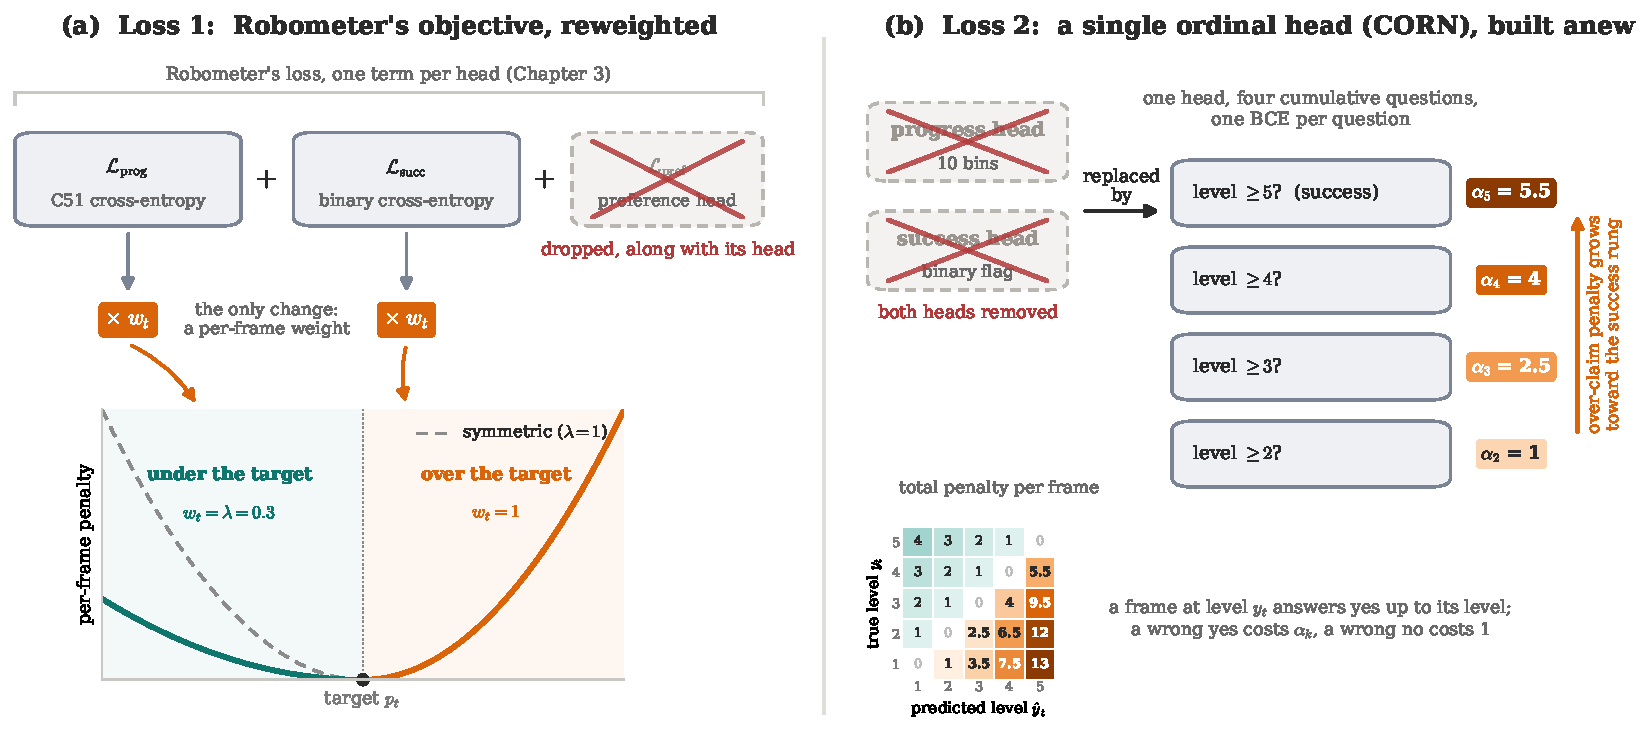
\includegraphics[width=\textwidth]{media/loss/asym_losses.pdf}
\caption[The two candidate loss objectives]{The two candidate objectives of Section~\ref{sec:method-loss}, drawn structurally. \emph{(a)} The first loss keeps Robometer's objective and its two task heads and only reweights them. The preference term is dropped together with its head, and each remaining term is multiplied by a per-frame weight $w_t$, equal to $1$ when the prediction sits above its target and $\lambda = 0.3$ when it sits below, which gives the asymmetric penalty of the lower plot, where an illustrative squared error stands in for the C51 cross-entropy. \emph{(b)} The second loss is built anew. It removes the progress and success heads entirely and replaces them with a single ordinal head that answers four cumulative questions, one binary cross-entropy per threshold, and claiming a level the frame has not reached costs $\alpha_k = 1 + c\,(k-2)$ with $c = 1.5$, heaviest at the success threshold. The matrix reads off the total penalty for every pair of true and predicted level, over-claims in orange, under-claims in teal, so the single most expensive mistake is claiming success on a frame with no progress at all.}
\label{fig:asym-losses}
\end{figure*}

\subsection{Reweighting Robometer's heads}

This objective keeps Robometer's two heads and their losses and adjusts only the weight on each frame's loss. When the model predicts too high, the frame keeps its full loss. When it predicts too low, the loss is scaled down by a factor $\lambda < 1$. An over-prediction therefore moves the weights more than an under-prediction of the same size, and the model drifts toward the low side of its targets. We use the same $\lambda$ on both heads, and $\lambda = 1$ gives back the ordinary symmetric loss. Figure~\ref{fig:asym-losses}~(a) shows the shape this induces around a target, a full-cost arm above it and a damped arm below.

On the progress head we compare, at each frame, the progress the model reports against the target. The reported value is the mean of its predicted distribution, $\bar{p}_t = \sum_{i=1}^{N} \hat{p}_{t,i}\,c_i$, with $\hat{p}_t$ the distribution over the bins with centers $c_i$ from Chapter~\ref{sec:robometer}, and $p_t$ is the target. We keep the same C51 cross-entropy as before and multiply it by a weight $w_t$ that is $1$ when $\bar{p}_t$ sits above the target and $\lambda$ when it sits at or below it,
\begin{equation}
\mathcal{L}_{\mathrm{prog}} = \frac{1}{T}\sum_{t=1}^{T} w_t\,\mathrm{CE}\!\big(\mathrm{Proj}(p_t),\, \hat{p}_t\big), \qquad
w_t = \begin{cases} 1, & \bar{p}_t > p_t,\\[2pt] \lambda, & \bar{p}_t \le p_t. \end{cases}
\label{eq:prog-asym}
\end{equation}
In Equation~\ref{eq:prog-asym}, this comparison of $\bar{p}_t$ against $p_t$ reads the current prediction only as a fixed reference, so it sets the weight for each frame without adding a gradient of its own.

On the success head over-prediction means one specific thing, calling a frame complete when it is not, so the same bias falls on the two label classes, not on a per-frame comparison. We keep the binary cross-entropy of Chapter~\ref{sec:robometer} and split it by the target. Frames that are genuinely incomplete, with $s_t = 0$, keep full weight, and frames that are complete, with $s_t = 1$, are damped by $\lambda$,
\begin{equation}
\mathcal{L}_{\mathrm{succ}} = \frac{1}{|\mathcal{N}|}\sum_{t \in \mathcal{N}} \mathrm{BCE}\!\big(0,\, \hat{s}_t\big) \;+\; \lambda\,\frac{1}{|\mathcal{P}|}\sum_{t \in \mathcal{P}} \mathrm{BCE}\!\big(1,\, \hat{s}_t\big),
\label{eq:succ-asym}
\end{equation}
In Equation~\ref{eq:succ-asym}, $\mathcal{N} = \{t : s_t = 0\}$ and $\mathcal{P} = \{t : s_t = 1\}$ are the unsuccessful and successful frames. Damping the positive class makes the model reluctant to fire a success signal, which is again the mistake we most want to suppress. A failed trajectory is unsuccessful at every frame, so all of its frames sit in the full-weight term $\mathcal{N}$, and the damped term is supplied by the successful trajectories the batch is paired with.

We use $\lambda = 0.3$ for both heads, so an under-prediction is corrected at less than a third of the strength of a matching over-prediction. Nothing else in this objective changes, and the heads, their targets, and the sum $\mathcal{L} = \mathcal{L}_{\mathrm{prog}} + \mathcal{L}_{\mathrm{succ}}$ are as in Section~\ref{sec:method-arch}, with the asymmetry living entirely in the two weights.

\subsection{Conditional Ordinal Regression for Neural Networks (CORN)}

The reweighting corrects the loss but leaves a deeper mismatch in place. Robometer's progress head predicts a distribution over ten bins and is trained by cross-entropy, which treats those bins as unordered categories. Nothing in the objective knows that the bins form a scale, that bin eight sits beside bin seven and far from bin one, so the penalty does not grow with how far a prediction lands from the target. The asymmetric weight of the previous section shares this blind spot, since it stamps a prediction as an over-prediction and applies full weight whether the model is a little too high or wildly too high. A conservative reward really wants the cost of over-prediction to scale with its size, and an ordinal formulation delivers that.

The second objective therefore replaces the ten-bin head with one that is ordinal by construction, following the rank-consistent CORN formulation \citep{shi_deep_2021}.
Instead of a distribution over bins, the head asks, for each frame, a short ladder of cumulative questions. It emits four logits $z_{t,k}$ for $k \in \{2,3,4,5\}$, and $\sigma(z_{t,k})$ is read as the probability that the frame's rubric level $y_t \in \{1,\dots,5\}$ is at least $k$. Decoding the thresholds in order recovers the level, and because they are cumulative a prediction that is off by one level fails a single threshold while one off by three fails three. Ordinal distance is now part of the loss, which is what the bin classifier lacked.

The label for a frame is that same set of yes-or-no answers. A frame at level $y_t$ answers yes to every threshold at or below its level and no to the rest, which we write as the cumulative bits $b_{t,k} = \mathbf{1}[y_t \ge k]$. For instance, a frame at level three is at least two and at least three but not four or five, so its four answers are $(1,1,0,0)$. Each threshold is trained with its own binary cross-entropy, and the asymmetry enters as a weight $\alpha_k$ on the term that fires when the true level is below the threshold, the case where the model over-claims. A single hyperparameter $c \ge 0$ fixes these weights through $\alpha_k = 1 + c\,(k-2)$, so they grow with the level. Figure~\ref{fig:asym-losses}~(b) lays out the cost structure this produces over every pair of true and predicted level. The loss is
\begin{equation}
\begin{split}
\mathcal{L}_{\mathrm{prog}} = -\frac{1}{T}\sum_{t=1}^{T} \sum_{k=2}^{5} \Big[\, & b_{t,k}\,\log\sigma(z_{t,k}) \\
&+ \alpha_k\,(1 - b_{t,k})\,\log\big(1 - \sigma(z_{t,k})\big) \Big].
\end{split}
\label{eq:corn-asym}
\end{equation}
To conclude, the loss of Equation~\ref{eq:corn-asym} asks at every frame, for each level, whether the frame has reached that level, and scores each yes-or-no answer with an ordinary binary cross-entropy, just as the success head does. The only twist is that a wrong yes, claiming a level the frame has not reached, is charged more than a wrong no, and through $\alpha_k$ that surcharge is heaviest at the top level, the one that asks whether the task is finished. Setting $c = 0$ removes the asymmetry, and we use $c = 1.5$. We also try other sets of hyperparameters analyzed in Chapter~\ref{sec:results}.

This single head also does the work of two. The top rubric level is task completion, so its threshold already answers the success question, with $\sigma(z_{t,5})$ read as the probability that the task is complete at frame $t$. Robometer's separate progress and success heads collapse into one ordinal head, the lower thresholds carrying partial progress and the top threshold carrying success. So ultimately, for this loss we use a single head.

\subsection{Two additions around the loss}
\label{sec:method-extras}

Alongside the two objectives we design two further training-time additions, both aimed at weaknesses we expect, not weaknesses we have measured, and both evaluated in the comparison of Chapter~\ref{sec:results}.

The first is a KL anchor against forgetting the failures. Two asymmetries in our corpus push the model to drift away from its failure knowledge during training. Success labels are clean $t/T$ ramps while failure labels carry labeling-pipeline noise, so the optimizer gravitates toward the clean side, and the success pool outnumbers the failure pool several times over. The anchor counteracts this and it is a standard technique against catastrophic forgetting \citep{kirkpatrick_overcoming_2016, li_learning_2016}. We keep a small first-in-first-out buffer of recently seen failures together with the progress logits the model produced for them at the time. On every success step we re-score one buffered failure with the current weights and penalize movement away from the stored prediction,
\begin{equation}
\mathcal{L} = \mathcal{L}_{\mathrm{prog}} + \mathcal{L}_{\mathrm{succ}}
+ \lambda_{\mathrm{kl}}\, \mathrm{KL}\!\big(P_{\mathrm{old}} \,\|\, P_{\mathrm{new}}\big),
\label{eq:kl-anchor}
\end{equation}
where $P_{\mathrm{old}}$ is the stored progress distribution of the buffered failure, treated as a constant, and $P_{\mathrm{new}}$ is the distribution the current model assigns to the same input, so gradient flows only through the new prediction. The KL is the standard categorical divergence over the ten progress bins, averaged over the frames that carry labels, and $\lambda_{\mathrm{kl}}$ sets how strongly the past prediction binds the present one.

The second is dropout on the task description, applied only to samples that carry an in-context demonstration. With probability one third the description is kept as written, with probability one third it is replaced by a generic phrase such as ``perform the demonstrated task'', and otherwise every word is independently dropped with a small probability. The intent is to force the model to ground its judgment in the demonstration frames, since vision-language models are known to lean on the language prior instead of the visual evidence \citep{goyal_making_2017}.

\subsection{Choosing between the losses}

The two objectives differ in one practical respect. The reweighted loss is essentially identical in form to the original loss of Robometer, performing only a reweighting, so it can resume from the pretrained weights directly, while the ordinal objective has to learn its head from scratch, since four cumulative logits do not line up with the pretrained ten-bin progress head. To decide between them we finetune Robometer with both losses as LoRA adapters \citep{hu_lora_2022} under an otherwise identical recipe and compare them. As the results in Chapter~\ref{sec:results} show, the reweighted objective is the setting we adopt for the full fine-tunes, and Appendix~\ref{apx:lambda} breaks the comparison down in full, split by split, together with the sweep behind the asymmetry strength we adopt.

\section{Training and model variants}
\label{sec:method-training}

The LoRA comparison of Section~\ref{sec:method-loss} used lightweight adapters to choose an objective cheaply. The models we actually study are full fine-tunes of the language model and the reward heads, with the vision encoder kept frozen as in Robometer's own training, sharded across H100 GPUs with Fully Sharded Data Parallel (FSDP) in the bfloat16 floating-point format, on the re-curated dataset of Section~\ref{sec:method-dataset} and with the reweighted asymmetric loss that came out ahead. On top of this shared recipe we vary two things, where training starts from and how much of our method is switched on, which gives a small grid of models.

\subsection{Two starting points}

We train from two starting points to separate what our method adds from what Robometer's own reward pretraining already provides. The first is Robometer-4B. We load the released reward model together with its pretrained progress and success heads and continue training it on our data. The second starts from the base vision-language model, Qwen3.5-4B \citep{team_qwen35-omni_2026}, with freshly initialized reward heads and no reward pretraining at all. We use Qwen3.5-4B because it is a newer and stronger base model than the Qwen3-VL that Robometer builds on, so training a reward model on top of it aims for better results while also showing how much Robometer's existing reward pretraining is worth. Because its heads start cold, the Qwen3.5 model is trained in two phases, a first pass over the fuller corpus to settle the heads and a second on the same standard-arm pool the Robometer-4B runs use. Robometer-4B, already a reward model, is fine-tuned in a single pass.

\subsection{Model ablations}

For each starting point we train three versions that switch on our contributions one at a time, so each reads against the one before it. The first is a plain fine-tune on our data that keeps Robometer's original symmetric progress and success losses and adds no demonstrations, which isolates what the re-curated failure data alone has to offer. The second replaces those losses with the asymmetric loss function that was better in Section~\ref{sec:method-loss}, the one that reweighted Robometer's original loss. The third adds in-context demonstrations on top, with the per-sample coin flip of Section~\ref{sec:method-icl}, and is the full RoboRef model. Two starting points and three versions give six trained models, which Chapter~\ref{sec:results} evaluates against each other and against the untuned Robometer baseline and other reward models.

\subsection{Optimization}

We fine-tune with AdamW \citep{loshchilov_decoupled_2019}, weight decay $0.01$, and a cosine learning-rate schedule with a $10\%$ warmup, clipping gradients to a norm of $10$ and running in bfloat16 with gradient checkpointing. Each GPU carries eight trajectories, sharded across eight H100 GPUs on two nodes. The Robometer-4B runs use a learning rate of $10^{-5}$ for $5{,}000$ steps. The Qwen3.5 runs, warming a fresh head, run at $2\times10^{-5}$ for $6{,}500$ steps in the first phase (which matches the training of Robometer-4B on top of Qwen3-VL) and $10^{-5}$ for a further $5{,}000$ steps in the second. Each trajectory is sixteen frames, and a sample carrying a demonstration adds sixteen more, as in Section~\ref{sec:method-arch}.

All runs draw from the re-curated corpus of Section~\ref{sec:method-dataset}. The Robometer-4B models train on its standard-arm portion, roughly $649$k clips with the humanoid and human data held out, while the Qwen3.5 model sees the fuller corpus in its first phase before narrowing to that same portion in its second. We reason that the humanoid robot and human dexterity data have significant information to offer to a reward model, but are unnecessary to the last finetuning stage, as the model is evaluated only in single-arm manipulator setups. Instead of keeping the corpus's natural success-heavy mix, we oversample failures during training, roughly doubling how often they are drawn, which raises their share of what the model sees from $18\%$ to about $30\%$. This way we are increasing the impact of our additional failure data, and also better balance the success/failure ratio that is heavily in favor of successes in the original mix. Two sources get their own factors on top, DROID failures because they are our scarcest real-world failures and MetaWorld successes because that source is almost all failures and its few successes would otherwise barely appear. For FailSafe we do not apply oversampling since the data come from only three tasks and that could lead to overfitting. The exact factors are listed in Appendix~\ref{apx:roboref-data}. The window subsampling and the four sample-generation strategies of Chapter~\ref{sec:robometer} are kept unchanged.

        \chapter{Results}
\label{sec:results}

A reward model is only as useful as the policies it can train. Offline metrics ask how well it scores trajectories it is handed, but a foundation reward model is meant to be deployed, and in deployment it is queried by an optimizing policy on that policy's own rollouts. That is the setting we care about most, and, as this chapter shows, it is also the one that separates the models most sharply. We build toward it in stages. We first run lightweight comparisons to settle the training recipe, then evaluate the resulting models offline on both in-distribution and out-of-distribution data, and finally use them as the reward signal for downstream reinforcement learning. The central result is a gap between the two regimes, strong offline scores that do not carry over on-policy, and much of the chapter is spent measuring that gap and explaining where it comes from. Throughout, the findings are tied back to the four research questions of the introduction, whether failure data improves the discrimination of success from failure (RQ1), whether an in-context demonstration improves the model's judgment (RQ2), whether an asymmetric loss tames overconfidence and makes the reward harder to exploit (RQ3), and whether offline gains transfer to downstream reinforcement learning (RQ4), and each is restated briefly where it is answered. The recipe and offline sections carry most of the evidence for RQ1 and RQ2, and the downstream sections decide RQ3 and RQ4.

\section{Experimental setup}
\label{sec:exp-setup}

\subsection{Models and baselines}

We evaluate the six fine-tuned models of Section~\ref{sec:method-training}, the two backbones, Robometer-4B and Qwen3.5-VL-4B, each trained in three versions that add one contribution at a time: the standard symmetric loss fine-tuned on our failure data, the asymmetric loss in its place, and finally the addition of in-context demonstrations. Our reference point throughout is the off-the-shelf Robometer-4B, the released reward model before any of our training. On the out-of-distribution set described below it reproduces the numbers reported in the Robometer paper, which validates our evaluation setup. Section~\ref{sec:results-lora} settles the loss these six models share before we train them at full scale.

\subsection{Offline evaluation}

Offline we ask two things of a reward model. The first is whether it orders trajectories correctly, ranking a successful attempt above a failed one and a later frame above an earlier one, where the latter case is only for successful trajectories. We measure this with rank accuracy, the fraction of success-failure pairs the reward orders the right way, and with Kendall's $\tau$ between predicted progress and true frame order. The second is whether the success head, the signal a downstream policy actually reads, separates success from failure at the level of a single frame. Here we report the area under the ROC curve (ROC-AUC) and, to account for the (slight) class imbalance, the area under the precision-recall curve (AUPRC). Most importantly, we report the true-positive rate at a strict five-percent false-positive budget ($\mathrm{TPR}@5\%\,\mathrm{FPR}$). To compute it we sweep the decision threshold over the pooled scores of the evaluation split until five percent of failure frames land above it, then report the fraction of success frames clearing that same cut, so the false-positive rate is fixed by construction and the true-positive rate is what the model achieves at that threshold. This represents the practical operating point for downstream reinforcement learning. Because a strictly zero-percent false-positive threshold in high-dimensional domains typically suppresses the true-positive rate to the point of destroying the learning signal, we accept a 5\% margin to capture more genuine successes.

For the progress head we also report class separation as $d' = (\mu_{\mathrm{succ}} - \mu_{\mathrm{fail}})/\sigma$, the distance between the mean success and mean failure score in pooled standard deviations. A reward can rank pairs correctly on average and still overlap the two classes enough for a false positive to slip through at the threshold a policy uses, and $d'$ is what tells the two situations apart. Every metric in this chapter, offline and downstream alike, is oriented so that higher is better.

We compute every offline metric on two splits. The first is in-distribution, a held-out portion of our own re-curated data. The second is out-of-distribution, the held-out-embodiment evaluation set from Robometer, made of real-world robots and scenes that appear in neither model's training. The two splits behave very differently, and the contrast between them is itself one of the chapter's findings.

\subsection{Downstream reinforcement learning}

The deployment test is downstream reinforcement learning. We train image-based policies with IBRL \citep{hu_imitation_2024}
and replace the sparse binary environment reward with the reward model, querying it on the policy's own rollouts. IBRL bootstraps an off-policy actor-critic, here soft actor-critic \citep{haarnoja_soft_2018}, from a behavior-cloning policy trained on the same demonstrations, which it also keeps in the replay buffer alongside the agent's own rollouts. The off-policy nature of the backbone is of specific importance. An off-policy critic is sensitive to the form a dense reward takes, not only its ranking, and it can bootstrap value from a spurious early terminal, the exploit the minimum episode length is there to close. A run is scored by the task success rate of the policy it produces. As a control we run the identical loop with the simulator's ground-truth reward, which bounds what the setup can reach when the reward is perfect and isolates the reward as the variable under test. We consider two common but different training setups with different policy backbones. One learns from sparse, binary rewards that mark task success, read from the success head, and the other from dense, continuous rewards that track task progress, read per step from the progress head. In both we sweep the weighting and threshold that turn the model's output into a scalar reward. We evaluate on three simulated manipulation benchmarks to test varying degrees of distribution shift. MetaWorld \citep{yu_meta-world_2019, mclean_meta-world_2025} serves as an environment where our model holds an advantage, as the baseline was trained on significantly less MetaWorld data. It is held-out in-distribution in the strict sense, since the domain is familiar but the tasks we train on appear in no reward model's training data. LIBERO \citep{liu_libero_2023} is in-distribution for both reward models, held out at the task level only for the baseline, a provenance Section~\ref{sec:results-rl-libero} spells out, while Robomimic \citep{robomimic} tests both models in a strictly out-of-distribution setting. On MetaWorld and Robomimic the policy backbone is IBRL as described above, while on LIBERO we train with the soft actor-critic implementation released with Robometer, so the baseline is evaluated inside its authors' own reinforcement learning loop.

\section{Choosing the training recipe}
\label{sec:results-recipe}

The full fine-tunes commit to two choices ahead of time, the training objective and the frame budget. This section fixes both by experiment, and every section after it evaluates the models that come out.

\subsection{Choosing the loss}
\label{sec:results-lora}

We train LoRA \citep{hu_lora_2022} adapters of rank $32$ on the attention and MLP projections of Robometer-4B, together with the reward heads, on an $18$k-trajectory sample of the corpus, and evaluate every few hundred steps on held-out slices of each source, DROID, Robometer, MetaWorld, and FailSafe. The training sample has a similar success-failure ratio to the full dataset. The deciding metric is rank accuracy, the fraction of success-failure pairs the reward orders correctly, averaged over the four splits, the same aggregate we later use to compare the full fine-tunes. Every evaluation runs twice, with and without an in-context demonstration.

The study compares the two candidates of Section~\ref{sec:method-loss} and the additions built around them. The ordinal CORN loss runs at $c \in \{0, 0.5, 1.5\}$, with its head freshly initialized because four cumulative logits cannot inherit the pretrained ten-bin head, and the reweighted loss at $\lambda = 0.3$ on top of Robometer's own heads. The hyperparameter for the reweighted loss is selected after a set of preliminary experiments, and Appendix~\ref{apx:lambda} reports the sweep against the milder $\lambda = 0.5$. Around this loss, we also test the task-description dropout and the KL anchor of Section~\ref{sec:method-extras}. We train each variant for 7,500 steps, and then compare each variant at its best checkpoint by the aggregate, the checkpoint that would be selected and carried forward in practice. Appendix~\ref{apx:lambda} breaks these aggregates down per split.

\begin{figure}[t]
\centering
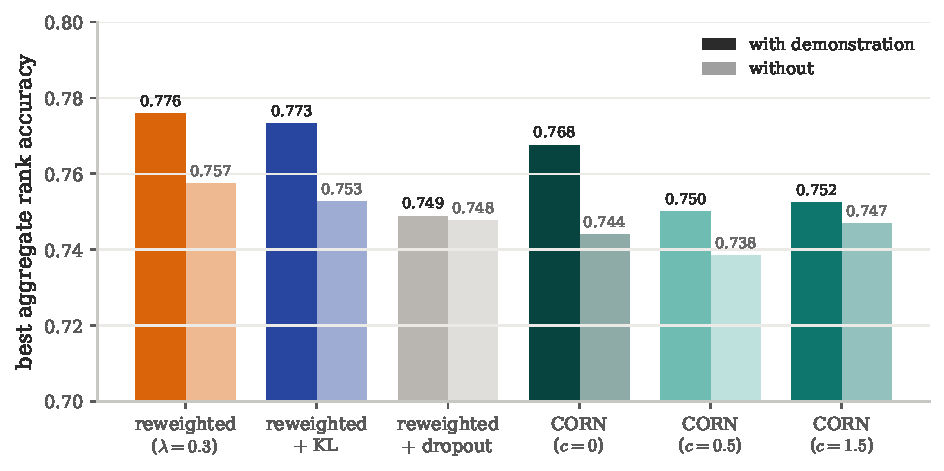
\includegraphics[width=\columnwidth]{media/results/lora_loss_comparison.pdf}
\caption[LoRA loss comparison]{The LoRA loss comparison, each variant at its best checkpoint by the aggregate metric, rank accuracy averaged over the four evaluation splits. The plain reweighted loss posts the highest aggregate of the study, and none of the additions, the ordinal head, task-description dropout, or the KL anchor, exceeds it. The symmetric CORN variant ($c=0$) stopped at three thousand steps, within the window where every variant reaches its peak. Higher is better.}
\label{fig:lora-loss}
\end{figure}

Figure~\ref{fig:lora-loss} compares those best checkpoints. The plain reweighted loss at $\lambda = 0.3$ posts the highest aggregate of the study, $0.776$ with a demonstration attached and $0.757$ without. The CORN family sits below it throughout, and its own ordering actually reveals that the penalization is damaging. The symmetric variant at $c = 0$, which is essentially a standard cross entropy loss, is the best of the three, and pushing the asymmetry up to $c = 0.5$ and $1.5$ makes it slightly worse, so the ordinal formulation pays for its conservatism in ranking quality where the reweighted loss does not. That is the comparison that matters for our purpose, since conservatism is the property we require of the loss, and between the asymmetric variants of each family the reweighted objective leads by a clearer $0.776$ to $0.752$ (CORN with $c=0.5$). Combined with the practical advantage that the reweighted objective resumes directly from Robometer's pretrained heads while the fresh ordinal head must learn its calibration from nothing, we select the reweighted loss for our full fine-tunings.

The two additions of Section~\ref{sec:method-extras} fail despite their well-documented motivation. The KL anchor of Equation~\ref{eq:kl-anchor} at $\lambda_{\mathrm{kl}} = 0.1$ peaks marginally below the plain reweighted run, $0.773$ against $0.776$, and a stronger $\lambda_{\mathrm{kl}} = 0.3$ is no better. We leave it out of the full runs, with the asterisk that the full-scale corpus is far bigger than this $18$k-trajectory sample. Even at a matched success-failure ratio, the anchor's usefulness could look different at that scale. Furthermore, the KL anchor is an expensive addition. Every time a success is seen, the sampled failure's prediction has to be recomputed with the current weights, which means either halving the already-maxed batch size to do this concurrently or paying for it sequentially. Because the anchor adds this overhead without a corresponding gain, we drop it.

The task-description dropout, meant to force the model onto the visual evidence of the demonstration instead of the text, costs about three points of best aggregate instead, $0.749$ against $0.776$, and since it deliberately damages a channel the deployed model relies on, we keep it off.

Gaussian noise on the success labels, drawn per frame at $\sigma = 0.1$ with the endpoints pinned to zero and one, targets a different concern, that the model could learn to tell successes from failures by the shape of the target alone, a smooth ramp against a broken one, and not by content (Section~\ref{sec:method-dataset}). Figure~\ref{fig:label-noise} illustrates the scheme on schematic targets. It neither rescues the CORN head it is paired with nor improves the reweighted loss, and it blurs an otherwise clean training signal, so it too is dropped, the suboptimal outcome Chapter~\ref{sec:methodology} anticipated.

\begin{figure*}[t]
\centering
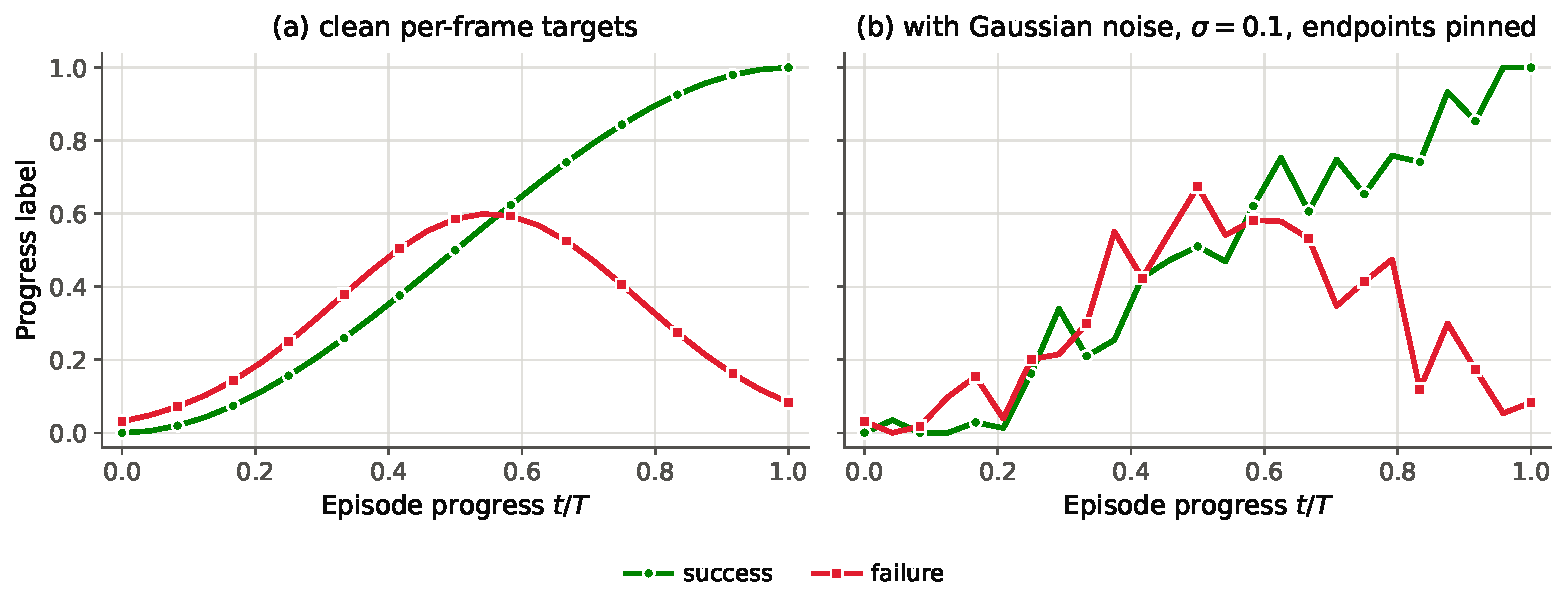
\includegraphics[width=0.92\textwidth]{media/results/label_noise.pdf}
\caption[Gaussian label noise]{The label-noise variant of the recipe study, illustrated on schematic targets. \emph{(a)} Clean per-frame progress targets for a successful and a failed episode, separable by shape alone, a smooth ramp against a broken one. \emph{(b)} The same targets with per-frame Gaussian noise at $\sigma = 0.1$ and the endpoints pinned, which disguises the shape while preserving the labels the heads must learn. The addition neither rescued the ordinal head nor improved the reweighted loss, so it was dropped.}
\label{fig:label-noise}
\end{figure*}


The configuration that emerges is the one Section~\ref{sec:method-training} trains at full scale, the reweighted asymmetric loss with $\lambda = 0.3$ on both heads, no KL anchor, no task-description dropout, and no label noise.

\subsection{Eight or sixteen frames}
\label{sec:results-frames}

Section~\ref{sec:method-arch} doubles Robometer's frame budget from eight to sixteen. We therefore train an eight-frame variant of the full in-context model under an otherwise identical recipe, and compare.

\begin{figure*}[t]
\centering
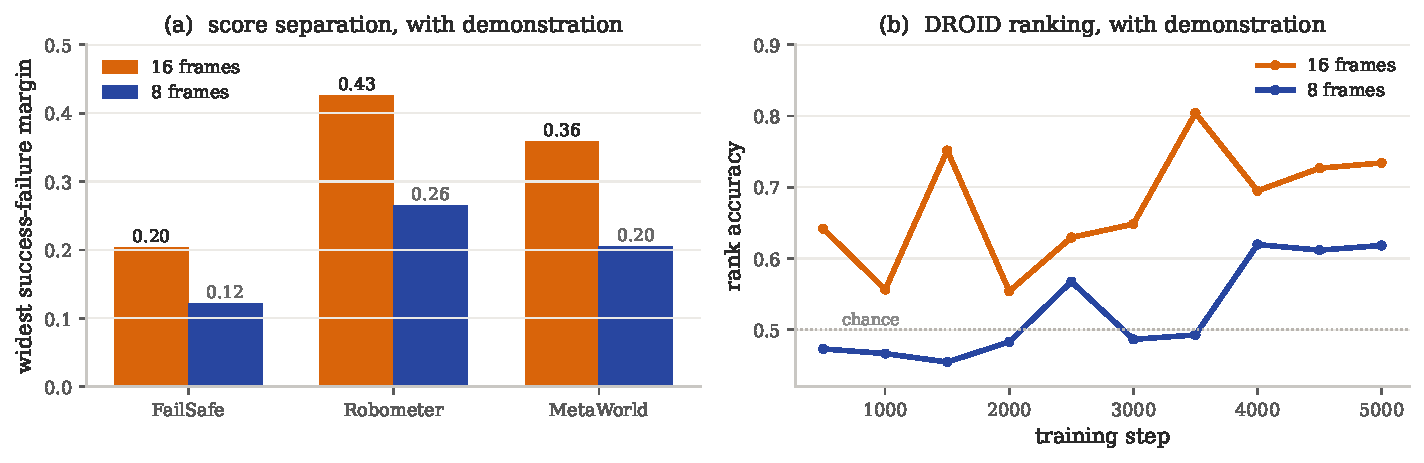
\includegraphics[width=\textwidth]{media/results/frames_8v16.pdf}
\caption[Eight versus sixteen frames]{The frame-budget ablation on the full in-context fine-tune, using the best asymmetric loss formulation. Both panels evaluated with a demonstration attached. \emph{(a)} The widest success-failure margin per split, where a task's margin is the mean score of its successes minus the mean score of its failures. Sixteen frames widen the best margin substantially on all three splits. \emph{(b)} Rank accuracy on DROID over training, where the sixteen-frame model leads at every evaluation. Higher is better in both panels.}
\label{fig:frames}
\end{figure*}

Figure~\ref{fig:frames} depicts the impact of using more frames. With a demonstration attached, sixteen frames widen the best success-failure margin substantially on all three shown splits, $0.12$ to $0.20$ on FailSafe, $0.26$ to $0.43$ on Robometer, and $0.20$ to $0.36$ on MetaWorld, and the mean margin across tasks moves in the same direction. Panel~(b) turns to DROID and to rank accuracy, the share of success-failure pairs the reward orders correctly, where the sixteen-frame model leads at every evaluation and finishes at $0.734$ against $0.620$. DROID is a special case, as it is the only real-world dataset and is significantly more difficult, so the comparison shows that more frames help most exactly where the data is toughest. One reason is more visual information. Another is temporal resolution. The moment that decides a real-world clip's score, a slipping grasp or a dropped object, can fall between two of eight frames and vanish, and with a demonstration attached the benefit compounds, since the demonstration's resolution doubles too. We keep sixteen frames for all six production runs.

\section{Offline reward quality}
\label{sec:results-offline}

Our position throughout this thesis is that downstream reinforcement learning is the evaluation that matters. We still measure offline quality first, for two reasons. It compares our six models and the released baseline on the footing prior work reports, and the gap between what it predicts and what the downstream evaluation later shows is itself one of this chapter's findings. We evaluate on the two splits of Section~\ref{sec:exp-setup}, one held out from our own corpus and therefore held in-distribution, and Robometer's held-out-embodiment set, out of distribution for every model in the table. Every model is scored with and without an in-context demonstration, including the models that never trained with one. Running both isolates the contribution of the demonstration itself, and the control is not empty for the released baseline, whose pretraining included a preference objective that presented two rollouts jointly, so a demonstration alongside the query is not an entirely unfamiliar input and could in principle help it.

\begin{table}[t]
\centering\footnotesize
\caption[Offline ranking, in-distribution]{Offline ranking, in-distribution, by the progress head. Rank accuracy is the fraction of success-failure pairs ordered correctly, $\tau$ is Kendall's correlation with true frame order. Both are reported with and without an in-context demonstration, including for the Qwen3.5 models that never trained with one. Higher is better for both metrics.}
\label{tab:offline-id-rank}
\begin{tabular}{@{}lcccc@{}}
\toprule
 & \multicolumn{2}{c}{no demonstration} & \multicolumn{2}{c}{with demonstration} \\
Model & rank-acc & $\tau$ & rank-acc & $\tau$ \\
\midrule
Robometer-4B (released) & 0.611 & 0.437 & 0.625 & 0.397 \\
RoboRef-ICL & 0.821 & \textbf{0.707} & \textbf{0.896} & \textbf{0.818} \\
RoboRef-Asym & \textbf{0.846} & 0.692 & 0.731 & 0.741 \\
RoboRef-Std & 0.771 & 0.591 & 0.747 & 0.672 \\
Qwen3.5-FT (asym $+$ ICL) & 0.834 & 0.669 & 0.842 & 0.676 \\
Qwen3.5-FT (asym) & 0.743 & 0.412 & 0.731 & 0.550 \\
Qwen3.5-FT (standard) & 0.813 & 0.617 & 0.693 & 0.398 \\
\bottomrule
\end{tabular}
\end{table}

\begin{table}[t]
\centering\footnotesize
\caption[Offline success detection, in-distribution]{Offline success detection, in-distribution. The success head is the signal downstream reinforcement learning reads, so its precision-recall area, its true-positive rate at a five-percent false-positive budget, and its ROC area are the numbers that matter most; $d'$ is the class separation of the progress head. Higher is better throughout.}
\label{tab:offline-id-succ}
\begin{tabular}{@{}lcccc@{}}
\toprule
Model & AUPRC & TPR@5\%FPR & ROC-AUC & $d'$ \\
\midrule
Robometer-4B (released) & 0.67 & 0.24 & 0.67 & 0.42 \\
RoboRef-ICL & \textbf{0.91} & \textbf{0.55} & \textbf{0.88} & \textbf{1.54} \\
RoboRef-Asym & 0.89 & 0.54 & \textbf{0.88} & 1.31 \\
RoboRef-Std & 0.88 & 0.51 & 0.87 & 1.08 \\
Qwen3.5-FT (asym $+$ ICL) & 0.69 & 0.23 & 0.69 & 0.54 \\
Qwen3.5-FT (asym) & 0.65 & 0.15 & 0.64 & 0.27 \\
Qwen3.5-FT (standard) & 0.64 & 0.14 & 0.65 & 0.32 \\
\bottomrule
\end{tabular}
\end{table}

In distribution, the RoboRef fine-tunes win across the board (Tables~\ref{tab:offline-id-rank} and~\ref{tab:offline-id-succ}). The operating point we care about most is the strict five-percent false-positive budget, where the reward must catch successes without paying out on failures, and there the fine-tuned models recover $0.51$ to $0.55$ of true successes against the baseline's $0.24$. We weight this metric most heavily because even our fine-tuned models remain overconfident despite the asymmetric loss, so the operating point that matters is the one that separates the classes without letting enough false positives through to poison an RL policy. The demonstration columns of Table~\ref{tab:offline-id-rank} also settle the control from the setup. The models that never trained with a demonstration mostly lose rank accuracy when one is attached, while the released baseline's small gain, $0.611$ to $0.625$, is consistent with its preference-era exposure. Its preference head taught it to read two trajectories in one input, a skill our non-ICL fine-tunes inherited but then partly lost, since they drop that head and never see a second trajectory again, ordinary catastrophic forgetting under fine-tuning. Either way, none of this approaches the jump the model trained with demonstrations shows. The benefit of in-context learning is earned in training, not granted by the input.

RoboRef-Std, which changes nothing of Robometer's recipe but the training data, isolates what the failure data alone contribute, and the contribution is large. Rank accuracy rises from $0.611$ to $0.771$ and the TPR at the same FPR threshold is more than double, going from $0.24$ to $0.51$. Adding the asymmetric loss on top improves every metric further, and adding the demonstration improves $d'$ most of all, $1.08 \to 1.31 \to 1.54$ across the three RoboRef fine-tunes. That progression matters because $d'$ is a very significant metric. A reward can rank the average success above the average failure and still let a policy find the overlap between the two distributions given an unstable standard deviation, so a demonstration that widens $d'$ is directly shrinking the false-positive rate available for a policy to exploit.

The headline result is that RoboRef-ICL is the best performing model overall, leading on $d'$ and on almost every other metric, and beating the baseline by more than $27$ percentage points in rank accuracy when a demonstration is given. It is also the most robust model without one, posting the best Kendall's $\tau$ of the field, evidence that training with a coin flip over whether to attach a demonstration, so the model works in both regimes, pays off. The one metric where it is not the best is rank accuracy without a demonstration, and only by a small margin. Finally, the suboptimal performance of the baseline is surprising considering the strong offline reward metrics reported in Robometer's paper. RBM-1M contains 100 demonstrations of MetaWorld tasks, far smaller than our own MetaWorld set. However, it still means that during training it has seen MetaWorld examples, making this inferior performance noteworthy.

The Qwen3.5 models, trained from cold heads without Robometer's reward pretraining, are close to the baseline's results on the success head and below their RoboRef counterparts on most metrics, most clearly in Table~\ref{tab:offline-id-succ}. The Qwen3.5-FT model trained with in-context learning is the standout among them, reaching $0.834$ rank accuracy without a demonstration, yet its success head (Table~\ref{tab:offline-id-succ}) is markedly weaker. Whether this gap reflects the base model or the missing reward pretraining is not something our experiments can separate. A Qwen3.5 model pretrained on Robometer's own recipe before our fine-tuning would answer this question, but that is beyond our compute budget, so the rest of this thesis centers on the stronger RoboRef models.

\begin{figure*}[h]
\centering
\begin{minipage}{\textwidth}
  \centering
  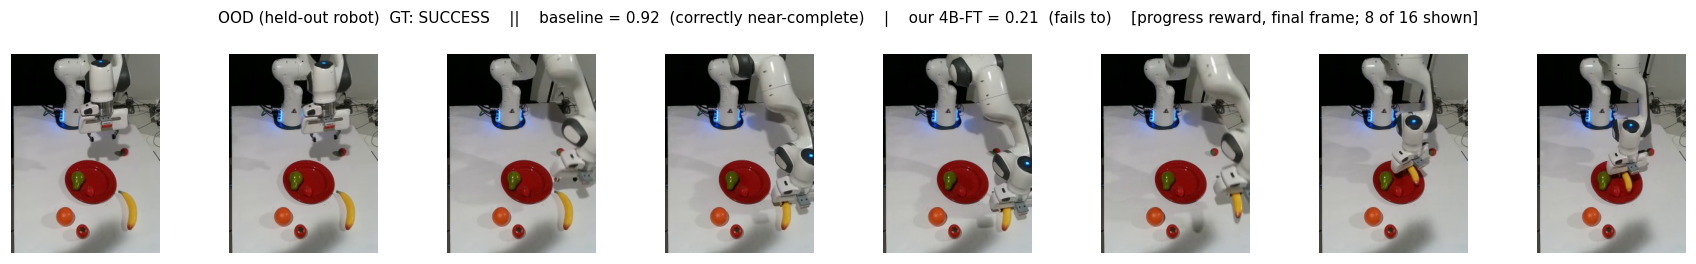
\includegraphics[width=0.93\textwidth]{media/results/ood_example.png}\\[2pt]
  {\footnotesize (a) out of distribution, the task ``Put banana on plate'' on a held-out robot, annotated a success in the evaluation set itself. Baseline $0.92$, ours $0.21$.}\\[6pt]
  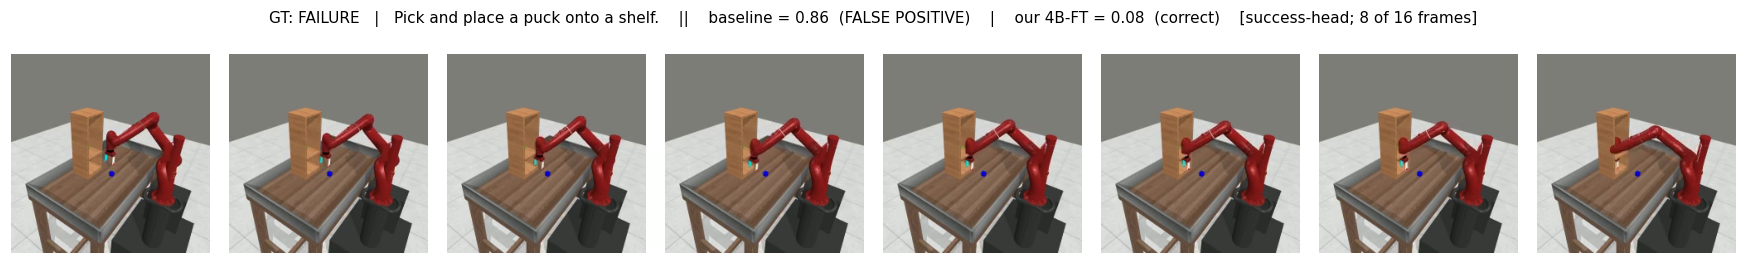
\includegraphics[width=0.93\textwidth]{media/results/id_fp_example.png}\\[2pt]
  {\footnotesize (b) in distribution, a failed attempt to pick up a puck and place it onto a shelf. Baseline $0.86$, a false positive; ours $0.08$.}
\end{minipage}
\caption[Offline trade-off on two clips]{The offline trade-off on two single clips, progress and success read on the final frames with the standard expectation readout for both models. \emph{(a)} Out of distribution the released baseline recognizes a completion our fine-tune appears to miss; the low value is largely the expectation readout compressing the fine-tune's bimodal output (Appendix~\ref{apx:condmean}). \emph{(b)} In distribution the baseline pays out on a failure our fine-tune correctly rejects.}
\label{fig:offline-qual}
\end{figure*}

Figure~\ref{fig:offline-qual} compares the baseline against our headline model, RoboRef-ICL. The upper plot reads the progress head on a successful out-of-distribution trajectory. The lower plot reads the success head on a failed in-distribution one. Two things stand out. First, the baseline scores both clips high, $0.92$ for the success and $0.86$ for the failure, which reveals its sensitivity to false positives. A genuine failure should not sit this high on the 0-1 scale, as well as this close to a genuine success, even if some threshold between $0.92$ and $0.86$ would technically separate them. Second, our model does separate the two with a cleaner margin, but notice that its own output is much smaller even on the success. The compression is not the model's judgment but an artifact of the standard readout on our model's bimodal output, which we return to shortly.



\begin{table}[h]
\centering\footnotesize
\caption[Offline reward metric evaluation, out of distribution]{Offline reward metric evaluation, out of distribution, on a $571$-episode held-out-robot set spanning six robots none of the models saw in training. The first two columns read the success head, its ROC area and its true-positive rate at a five-percent false-positive budget. The last two read the progress head, decoded as the mean conditioned on the model having moved off its lowest bin, since the fine-tuned heads' distributions are bimodal on this set (Appendix~\ref{apx:condmean}). Higher is better throughout.}
\label{tab:offline-ood}
\setlength{\tabcolsep}{3.5pt}
\begin{tabular}{@{}lcccc@{}}
\toprule
 & \multicolumn{2}{c}{success head} & \multicolumn{2}{c}{progress head} \\
\cmidrule(lr){2-3}\cmidrule(lr){4-5}
Model & AUC & TPR@5\% & rank-acc & $\tau$ \\
\midrule
Robometer-4B (released) & \textbf{0.86} & 0.38 & \textbf{0.81} & \textbf{0.63} \\
RoboRef-ICL & 0.84 & \textbf{0.40} & 0.75 & 0.50 \\
RoboRef-Asym & 0.79 & 0.28 & \textbf{0.81} & 0.58 \\
RoboRef-Std & 0.76 & 0.16 & 0.76 & 0.50 \\
Qwen3.5-FT (asym $+$ ICL) & 0.69 & 0.24 & 0.70 & 0.14 \\
Qwen3.5-FT (asym) & 0.66 & 0.16 & 0.64 & 0.28 \\
Qwen3.5-FT (standard) & 0.66 & 0.16 & 0.59 & 0.23 \\
\bottomrule
\end{tabular}
\end{table}

Subsequently, we compare our RoboRef variants directly with a released OOD dataset from Robometer on Table~\ref{tab:offline-ood}. Robometer's baseline leads three of the four columns, but only by a few points on rank accuracy and Kendall's $\tau$, and at the operating point we care about most, the true-positive rate at a five-percent false-positive budget, our headline model, RoboRef-ICL, actually edges past it, $0.40$ against $0.38$. Also, the Qwen3.5 variants demonstrate a disappointing performance in comparison to the RoboRef models, which reinforces our decision to continue only with the RoboRef models for the rest of the chapter.


One computational note applies to the progress columns that we briefly mentioned before. The fine-tuned heads produce bimodal bin distributions on this set, and the released readout, the expectation over the bins, collapses under that shape, so we decode every model with the conditional mean instead, the same expectation taken after the lowest bin is dropped and the rest renormalized. The change leaves the baseline's numbers untouched, its distributions are unimodal, and it lifts the asymmetric model's Kendall's $\tau$ from $0.16$ to the $0.58$ reported in the table. Appendix~\ref{apx:condmean} explains the readout, shows the distributions behind it, and answers why the in-distribution tables do not need it.

\begin{figure*}[t]
\centering
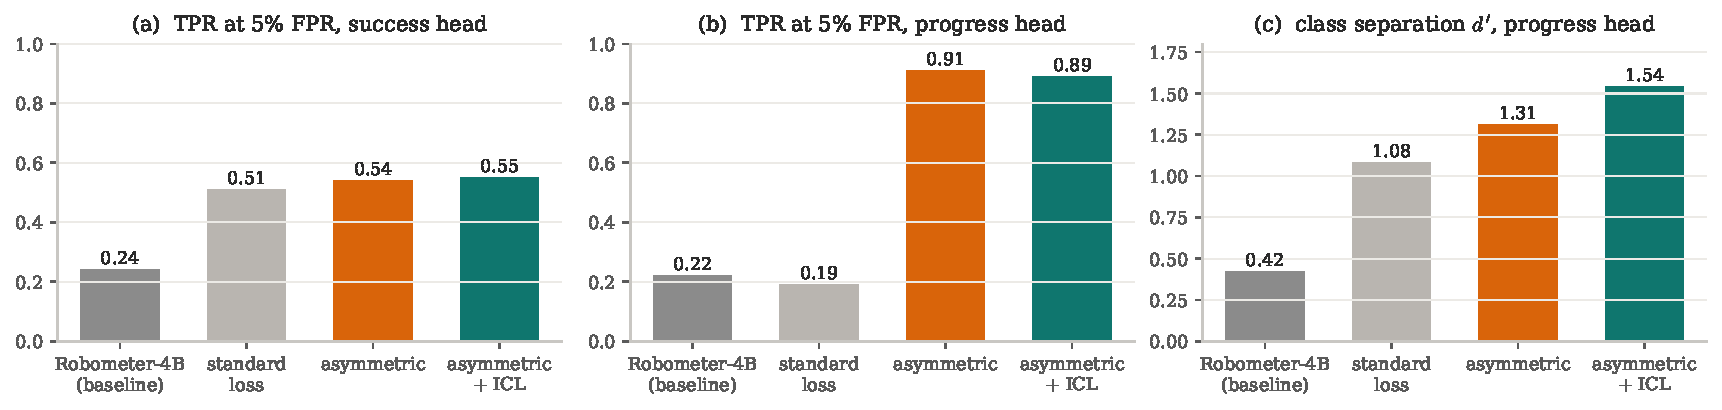
\includegraphics[width=\textwidth]{media/results/asym_offline.pdf}
\caption[What the asymmetric loss buys offline]{What the asymmetric loss buys on the in-distribution evaluation, isolated by comparing the three RoboRef fine-tunes against the released baseline. \emph{(a)} True-positive rate of the success head at a five-percent false-positive budget. \emph{(b)} The same operating point on the progress head. \emph{(c)} Class separation $d'$ between success and failure scores. The standard-loss fine-tune improves the success head but leaves the progress head unusable at a strict false-positive budget; the asymmetric loss delivers on both heads and separates the classes most cleanly. Higher is better in every panel.}
\label{fig:asym-offline}
\end{figure*}

\begin{figure*}[t]
\centering
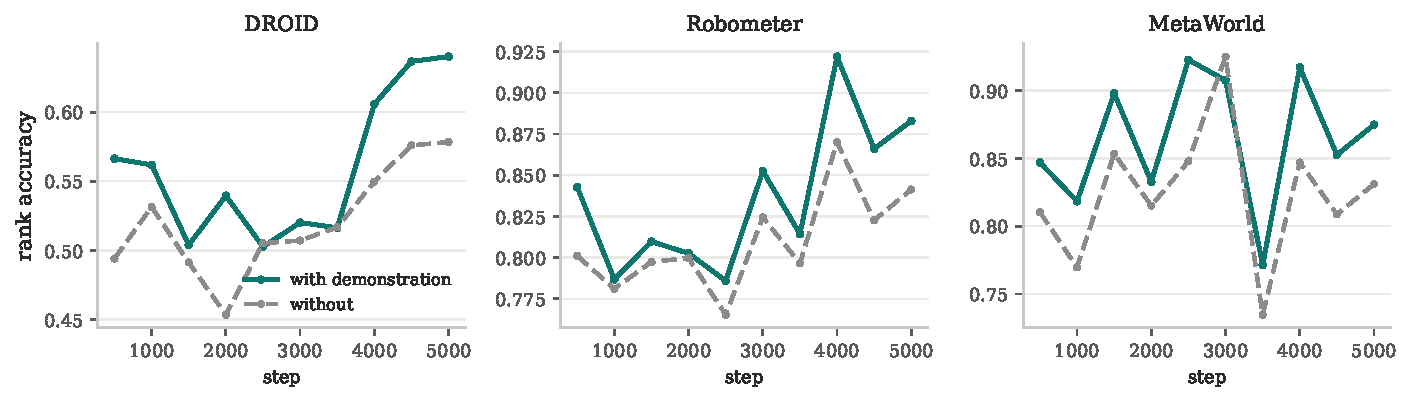
\includegraphics[width=\textwidth]{media/results/icl_convergence.pdf}
\caption[In-context demonstrations over training]{Rank accuracy over training for the full in-context model, evaluated with and without a demonstration, per evaluation split. The demonstration-conditioned evaluation leads on every split for essentially all of training, with the largest margin, still growing at the end, on DROID, the one real-world split. Higher is better.}
\label{fig:icl-convergence}
\end{figure*}

Set beside the in-distribution tables, there is a sharp contrast. There the RoboRef models lead every metric by a wide margin. Here, the baseline leads most of them and RoboRef-Std, already the weakest of the three RoboRef models in distribution, is again the weakest here, trailing on every column but rank accuracy. The reason is the ordinary cost of fine-tuning on a narrower, arm-focused corpus. Sharpening the model's judgment on the data it was trained on trades away some of the released model's broader visual coverage. Moreover, an interesting note is that since this dataset is OOD it should depict the robustness of Robometer-4B in various datasets. However, as we reported before, its performance in our in-distribution dataset, composed of MetaWorld, DROID, FailSafe, and Robometer, where all datasets are also in-distribution for the baseline, shows that the baseline is not as robust as the OOD dataset was suggesting. The asymmetric loss and the in-context demonstration still perform strongly here despite that cost, which is why the model that carries both, our headline model, matches or beats the baseline at the one operating point that matters most for downstream use, the strict-budget true-positive rate.


For the asymmetric loss, the cleanest comparison is between the three RoboRef fine-tunes, identical in everything but the objective, and Figure~\ref{fig:asym-offline} shows that it delivers by far the best class separation. On the success head, panel~(a), the true-positive rate at a five-percent false-positive budget rises from $0.51$ under the standard loss to $0.54$ and $0.55$ under the asymmetric ones, more than doubling the baseline's $0.24$. The progress head, panel~(b), is where the loss matters most, since the standard-loss variant recovers only $0.19$ of successes at that budget, no better than the released baseline, while the asymmetric models recover about $0.9$, and $d'$, panel~(c), rises from $1.08$ to $1.31$ without demonstrations and $1.54$ with them. The loss compresses the score scale yet overlaps the classes less, which is exactly the conservative shape it was designed to produce, and out of distribution the asymmetric variants are still the stronger pair, clearly ahead of the standard-loss fine-tune on the success head and on the constrained FPR operating point (Table~\ref{tab:offline-ood}). Although RQ3, the overconfidence question, mainly targets the RL experiments, the offline reward metric results depict that an asymmetric loss leads to better class separation and stronger true-positive rates at certain thresholds, which is one of our surprising, but positive, findings of this thesis.


\section{What the failure data and the demonstrations contribute}
\label{sec:results-icl}

RQ1 asks whether supervising the reward model on curated failure trajectories improves its ability to discriminate success from failure. In distribution the answer is unambiguous. As Section~\ref{sec:results-offline} showed, changing nothing about Robometer's recipe but the training data lifts rank accuracy by sixteen points and doubles the strict-budget true-positive rate, gains from the failure data alone. Out of distribution the same model trails the baseline on every column of Table~\ref{tab:offline-ood}, but the set itself is a coarse, $571$-episode policy-ranking benchmark, only $166$ of which are labeled outright failures, not the dense failure supervision our own corpus provides, so it is a weak test of what the failure data can do. We do not extend the offline evaluation further to chase a better one, since the test that matters most, downstream reinforcement learning, is next.

The comparison above isolates the data while keeping the loss fixed. One extra experiment closes the loop from the other side, keeping the data fixed and changing only the loss. We continued training the released model on its own corpus, with our added sources removed, under the same recipe as RoboRef-Asym, the same step budget, and the same checkpoint selection rule, so the only ingredient of ours it receives is the asymmetric loss. Table~\ref{tab:offline-abl} scores it on both evaluation splits. 

The loss alone moves almost nothing, and this is clearest on the in-distribution split. Trained on Robometer's own corpus, the asymmetric loss lifts rank accuracy from the baseline's $0.61$ to $0.64$ and its Kendall's $\tau$ actually drops, while the identical recipe on our data reaches $0.85$ and $0.69$, a gap of more than twenty points that the objective alone clearly cannot produce. Out of distribution the picture repeats. The ablation stays within noise of the baseline on the success-head area and on both progress columns, and at the strict false-positive budget it is clearly worse, because the loss reshapes the calibration without failure examples to separate the classes with. Robometer's corpus feeds the asymmetric terms very little, its failures enter training only as preference pairs, a few hundred batches over the whole run. Its progress head also keeps the unimodal shape of the released model, so the bimodal output our fine-tunes develop, the one Appendix~\ref{apx:condmean} studies, traces back to the failure data as well and not to the objective.

Up to this point the in-distribution gains could still be credited to the different loss function, since the asymmetric variants beat the standard one on every table. With both directions now tested, our data under their loss gains a lot and their data under our loss gains almost nothing, the credit falls on the failure data itself. The loss is an amplifier, and without our data it has nothing to amplify.

\begin{table}[h]
\centering\footnotesize
\caption[Loss-versus-data ablation]{The loss-versus-data ablation on both evaluation splits. The middle row trains the released model on its own corpus with our asymmetric loss and nothing else of ours. Its in-distribution scores come from the training pipeline's held-out evaluation at the selected checkpoint, computed on the same data sources as Table~\ref{tab:offline-id-rank}; the out-of-distribution columns use the held-out-robot set of Table~\ref{tab:offline-ood}. Its progress head stays unimodal, so the standard expectation readout applies to it, as it does to the baseline. Higher is better throughout.}
\label{tab:offline-abl}
\setlength{\tabcolsep}{2.5pt}
\begin{tabular}{@{}lcc@{\hskip 8pt}cccc@{}}
\toprule
 & \multicolumn{2}{c}{in-distribution} & \multicolumn{4}{c}{out of distribution} \\
\cmidrule(lr){2-3}\cmidrule(l){4-7}
 & \multicolumn{2}{c}{progress head} & \multicolumn{2}{c}{success head} & \multicolumn{2}{c}{progress head} \\
Model & rank-acc & $\tau$ & AUC & TPR@5\% & rank-acc & $\tau$ \\
\midrule
Robometer-4B (released) & 0.61 & 0.44 & \textbf{0.86} & \textbf{0.38} & \textbf{0.81} & \textbf{0.63} \\
$+$ our loss, their data & 0.64 & 0.36 & \textbf{0.86} & 0.16 & 0.80 & 0.60 \\
RoboRef-Asym (our data) & \textbf{0.85} & \textbf{0.69} & 0.79 & 0.28 & \textbf{0.81} & 0.58 \\
\bottomrule
\end{tabular}
\end{table}

Moreover, the in-context demonstration is the clearest single win in this chapter. With one attached, RoboRef-ICL reaches $0.896$ rank accuracy and $0.818$ Kendall's $\tau$ in distribution, more than $27$ percentage points above the baseline and the best number on almost every column of both in-distribution tables. Figure~\ref{fig:icl-convergence} scores RoboRef-ICL twice at every evaluation, with and without the demonstration attached. The demonstration wins on every split at essentially every stage of training, and by the largest margin on DROID, where the gap is still growing when training ends. The effect predates the full fine-tunes too, since every variant of the LoRA study already gained from a demonstration (Appendix~\ref{apx:lambda}). This mirrors the result of Figure~\ref{fig:frames} which suggested that the number of frames matters for harder tasks. Real-world clips pair cluttered scenes with terse task descriptions, so they benefit most from any additional information the input carries, whether more frames or a demonstration. The demonstration doubles the input length and with it the cost of a step, a price worth paying for a model meant to score real robots. In terms of RQ2, the demonstrations improve the model's judgment throughout, and most where the data is hardest.

The asymmetric loss is the other consistent winner. Across every offline table in this chapter, in-distribution ranking, in-distribution success detection, and out of distribution, the asymmetric variants beat the standard-loss fine-tune, with the class separation of Figure~\ref{fig:asym-offline} the clearest sign of it. The $d'$ of $1.31$ that the loss reaches without a demonstration matters on its own, since it shows the objective earns strong class separation with no help from in-context learning. We expect this conservatism to matter most once the reward is queried by an optimizing policy.

Taken together, the failure data supplies the signal, the demonstrations unlock it on real-world data, and the asymmetric loss turns it into a conservative, well-separated reward. Whether that survives an optimizing policy is the question the rest of the chapter takes up.

\section{Downstream reinforcement learning}
\label{sec:results-rl}

Everything so far has scored the reward models on data they were handed. The deployment test reverses that, letting an optimizing policy query the reward on its own rollouts, and it is the setting the whole chapter has been pointing toward. We evaluate on the three simulated benchmarks of Section~\ref{sec:exp-setup}, MetaWorld, LIBERO, and Robomimic. Because all three share the same reward configurations, we set those out first and refer back to them in each benchmark.

\subsection{Reward configurations}
\label{sec:results-rl-config}

The principle behind these configurations is that every reward model is run as its own authors intend, given its preferred inputs and its native reward form, instead of being forced into a single common protocol. Where the configurations differ they favour the baselines, not our models. The baselines are handed their richest inputs, a goal image and several camera views for one of them (RoboDopamine), a dense per-frame signal for two (RoboDopamine and LRM), and in one case a larger backbone than any of our own models (LRM, at eight billion parameters against our four), while our models are given nothing they were not already designed to use. Whatever advantage our models show is therefore a conservative one, measured against baselines running at their best, which is a harder test for us. Table~\ref{tab:rl-config} summarizes the settings, and the paragraphs below give the detail that the later sections refer back to.

\begin{table*}[t]
\centering\small
\setlength{\tabcolsep}{6pt}
\caption[Reward-model deployment configurations]{How each reward model is queried during reinforcement learning, shared across all three benchmarks. Our models act as success detectors that terminate an episode on detection. The baselines keep their native reward forms and preferred inputs, the configurations under which their authors report results, which favours them.}
\label{tab:rl-config}
\begin{tabular}{@{}lllll@{}}
\toprule
Model & Signal & Protocol & Conditioning & Size \\
\midrule
RoboRef & success head & autonomous, ends on detection & threshold, min length; ICL adds a demo & 4B \\
Robometer-4B & success head or dense progress & best form per benchmark & threshold, min length & 4B \\
RoboReward & rubric $1$--$5$ & full episode, reward at end & zero-shot & 4B \\
RoboDopamine & dense progress & full episode, dense & goal image, multiple views & 4B \\
LRM & dense progress & full episode, dense & initial-frame anchor & 8B \\
\bottomrule
\end{tabular}
\end{table*}

Our own models, RoboRef-Asym and RoboRef-ICL, are deployed the same way in all three benchmarks. They read the success head alone, as a sparse reward in the autonomous protocol of Section~\ref{sec:exp-setup}, and never the progress head, with the single exception of the LIBERO regime study that Section~\ref{sec:results-rl-libero} motivates separately. Every frame the policy produces is scored, and the moment the success probability crosses the model's threshold the episode is declared solved, terminating with the reward paid at that step alone. This is the ordinary way a reward model is used as a success detector, and it makes the reward's task unforgiving, since a single false fire both ends the episode prematurely and pays out a reward the policy never earned. The model has to be right about success and, just as importantly, silent about everything else.

Turning a continuous probability into that fire-or-not decision needs a threshold. A threshold is not particular to our reward; it is what any continuous score requires to act as a detector, and the models in this comparison emit their scores on plainly different scales, so a single shared cut would flatter one and starve another. We therefore calibrate one threshold per model, with an identical procedure for every model in the figure, ours and the baselines alike. On a small set of oracle rollouts collected once and kept out of training, we select the operating point that recovers the most true successes under a strict false-positive budget, the same conservative operating point we argued for offline. Because the recipe is shared, the calibration cannot be what separates the models, and whatever gap remains belongs to the reward itself. 

\begin{figure*}[t]
\centering
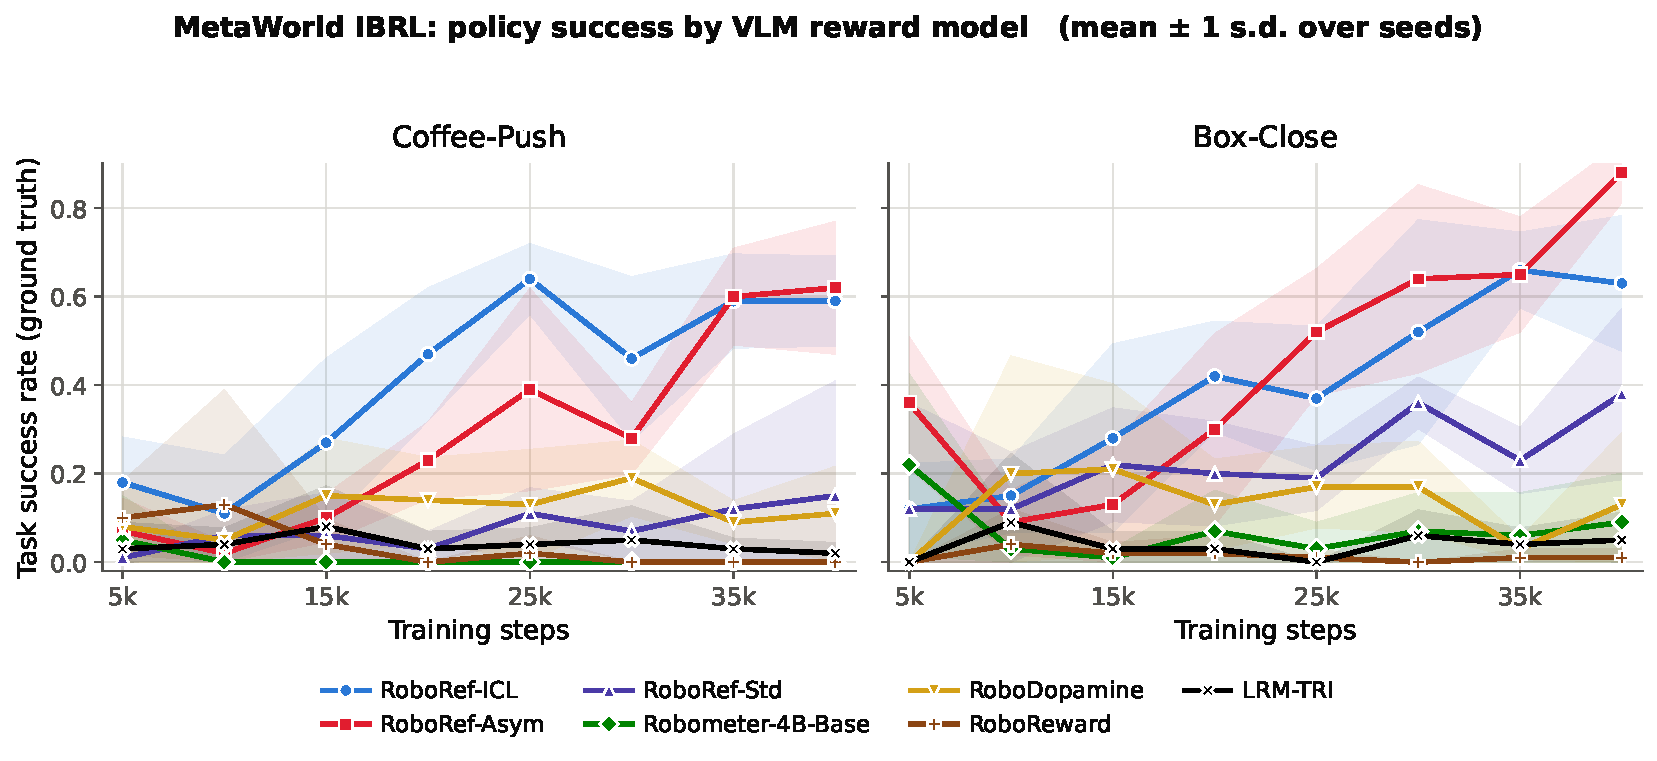
\includegraphics[width=\textwidth]{media/results/metaworld_rl.pdf}
\caption[MetaWorld downstream reinforcement learning]{MetaWorld downstream reinforcement learning, two held-out tasks absent from every reward model's training data, five seeds per reward, mean ground-truth success over training with a one standard deviation band. Success is true task success, measured where the reward model is never queried, not the reward the policy reads. Each reward runs in its Table~\ref{tab:rl-config} configuration, which favours the baselines, so the comparison is conservative for our models. Legend: RoboRef-ICL, RoboRef-Asym, and RoboRef-Std are our fine-tunes with asymmetric-plus-ICL, asymmetric, and standard loss, and Robometer-4B-Base is the released baseline. Only the two asymmetric fine-tunes train a competent policy. Every other reward model ends far behind.}
\label{fig:mw-rl}
\end{figure*}

This calibration does read ground truth, a small set of labeled rollouts, which is a real cost to an otherwise zero-shot deployment, so it matters that the procedure is a convenience and not a requirement. We observe that among the different simulators and different tasks, all thresholds separating successes and failures can be found between 0.75 and 0.9, for both our deployment models. Specifically, RoboRef-Asym varies between 0.75 and 0.85 and RoboRef-ICL between 0.8 and 0.9. The behavior of the policy is a good indication of whether the threshold is too high or too low. A low threshold leads to false positives, failures recognized as successes, which lead to early terminations and flat ground truth evaluations. A high threshold leads to full episodes and minimal signal, as it means that no episodes, either successful or not, manage to surpass the threshold. Thus, this calibration is a technique to quickly find a good threshold for our model ablations and the other baseline VLM reward models, but is not strictly necessary to get a working model.

Furthermore, we fix a minimum episode length per task. IBRL rests on off-policy actor-critic updates, and those methods are susceptible to an early-training exploit, where a policy learns to provoke a spurious success in an episode's first few steps, before the task is physically solvable, collect the terminal reward, and reset. We saw this failure across the reward models, ours and the baselines alike. To overcome it and avoid a flat, dead policy, we ignore any success signal that fires before the episode reaches the minimum. As a simple heuristic, we set the minimum to the length of a demonstration of the given task, drawn from the set the IBRL policy is pretrained on. This encodes a plain physical prior, that nothing is solved faster than an expert solves it, so any earlier fire is spurious by construction. We experiment with minimums between $0.8$ of the demonstration length and the full length, the results in the next sections use the best configuration, and we return to this design choice in Chapter~\ref{sec:discussion}.


Alongside our own models, RoboRef-Asym and RoboRef-ICL, we run three published vision-language reward models, each in the configuration its authors intend. RoboReward \citep{roboreward} scores a whole rollout on a one-to-five rubric and returns a single reward at the episode's end. RoboDopamine \citep{robodopamine} and LRM \citep{TRI-reward-model} emit dense per-frame progress, which we deliver as a shaped increment, each given the input its design expects, a goal image and multiple camera views for the former and an initial-frame anchor for the latter. The comparison also carries the released Robometer-4B from before any of our training, together with our standard-loss fine-tuned ablation, so that within each benchmark a single figure isolates the released model, the failure data, the loss, and the demonstrations in turn. The released baseline is a special case among these, since its paper deploys the progress head as a dense reward while its success head also works as a sparse detector. We do not force one choice on it and instead report its stronger form on each benchmark, naming the form used in each section.

\subsection{MetaWorld}
\label{sec:results-rl-mw}

We begin with MetaWorld, the one environment where our model holds a clear data advantage. That advantage is one of domain, not of memorized tasks, since the two tasks we train on appear in no reward model's training data. We train image-based IBRL policies on these two held-out tasks, Coffee-Push and Box-Close, with five random seeds per reward model, our models reading the success head as a sparse reward under the protocol of Section~\ref{sec:results-rl-config}, and score each seed by the true success rate of the policy it produces, measured in a separate clean evaluation where the reward model is never queried. The curves of Figure~\ref{fig:mw-rl} therefore report ground-truth success, not the model's own reward. The minimum episode length of Section~\ref{sec:results-rl-config} sits at twenty-four steps on Coffee-Push and forty-five on Box-Close, exactly 80\% of the sampled demonstration length.

Figure~\ref{fig:mw-rl} is the widest separation in the thesis. Only RoboRef-Asym and RoboRef-ICL train a competent policy on either task. RoboRef-Asym reaches a mean success of $0.50$ on Coffee-Push and $0.72$ on Box-Close, and RoboRef-ICL holds the same band, $0.55$ and $0.60$. Nothing else comes close. The three published baselines stay under $0.13$ throughout, and the released Robometer-4B, strong enough offline to reproduce the numbers reported in its own paper, moves the policy almost nowhere under either of its forms, $0.00$ on Coffee-Push and $0.07$ on Box-Close at its better one, the sparse detector.

The curve that shows training on MetaWorld data is not the sole factor of this victory is RoboRef-Std, our own standard-loss fine-tune. It sees exactly our failure data and differs from the asymmetric models in the objective alone, and offline it looked the part, recovering half of all successes at the strict false-positive budget (Table~\ref{tab:offline-id-succ}). Under an optimizing policy it comes apart, $0.11$ on Coffee-Push and $0.32$ on Box-Close, well short of the asymmetric fine-tunes trained on the same trajectories. This is the disconnect the chapter has been circling, made concrete on a single pair of curves. Our hypothesis for it is explicit. A fixed test set measures how often a reward is right on average, while an optimizing policy hunts for the specific states where it is wrong, so a model with strong average metrics but exploitable errors, here the false positives the standard loss leaves standing, ranks and detects well offline yet is pulled apart on-policy. The whole distance between the standard and asymmetric fine-tunes is the loss, and it is precisely the distance the conservatism of the asymmetric objective was designed to cover. What read offline as a modest edge in class separation, a $d'$ of $1.08$ against $1.31$ (Table~\ref{tab:offline-id-succ}), is on-policy the line between a reward a policy exploits and one it cannot. This shows plainly what the asymmetric loss does. It does not make the reward more accurate on average; it makes the reward hard to exploit, and being hard to exploit, not offline accuracy, is what decides whether a policy can be trained.

Our hypothesis is that reward hacking is the key factor behind the failed policy learning of every baseline in the figure. Appendix~\ref{apx:mw-reward} traces where it hides by plotting the reward each policy actually received during training. In short, the released Robometer-4B pays the policy the most reward of any model on Coffee-Push while its true success rate stays at zero, the signature of farmed false positives, and the asymmetric fine-tunes pay a smaller reward that climbs together with genuine success. The appendix also verifies that the shared calibration and minimum episode length are not what separates the models, so the advantage sits in the reward itself.

\subsection{LIBERO}
\label{sec:results-rl-libero}

\begin{figure*}[p]
\centering
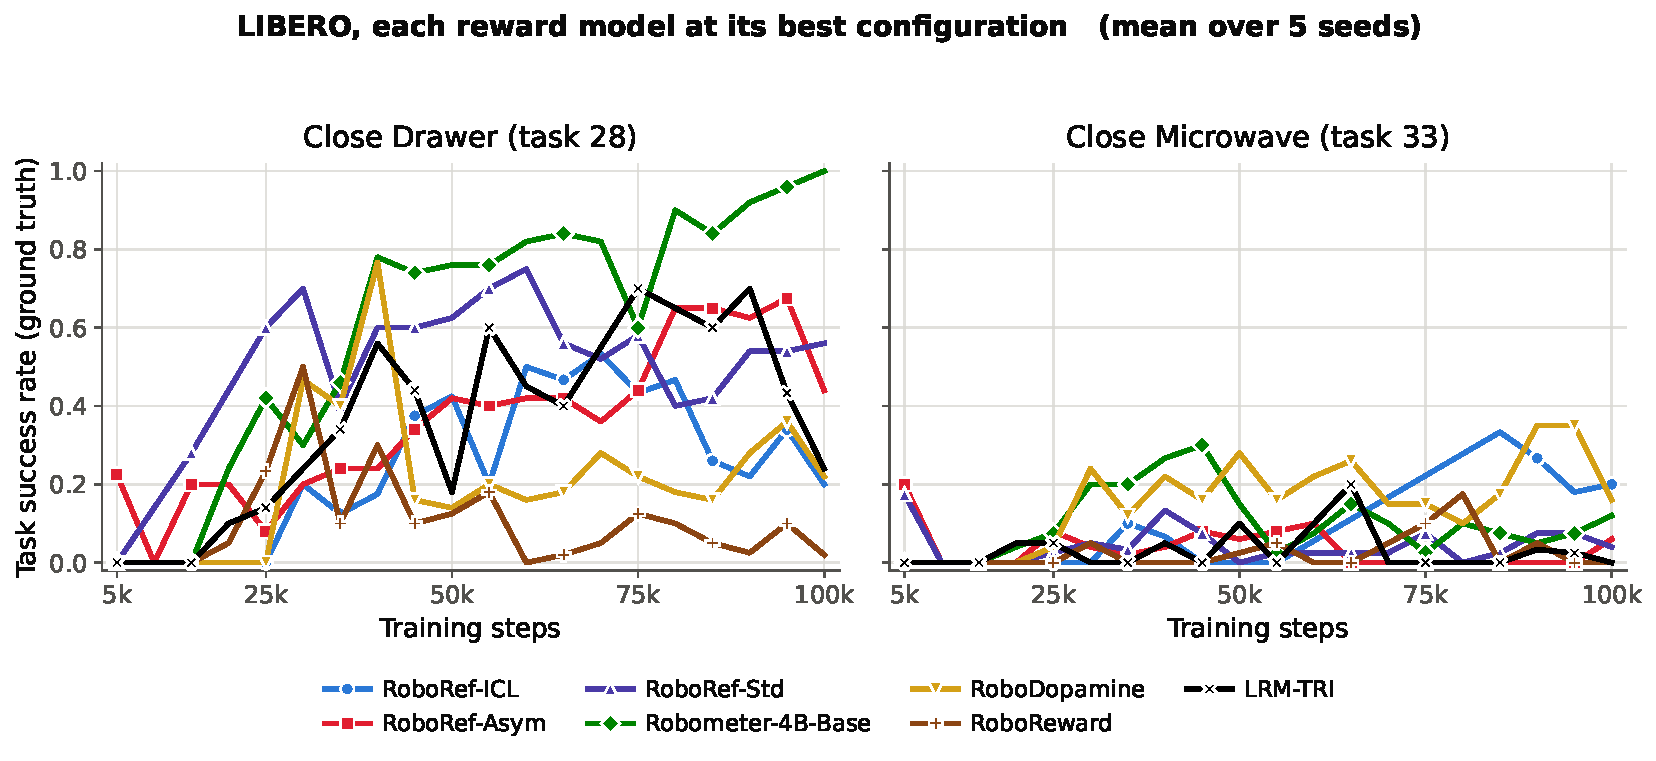
\includegraphics[width=\textwidth]{media/results/libero_rl.pdf}
\captionof{figure}[LIBERO downstream reinforcement learning]{LIBERO downstream reinforcement learning on Close-Drawer and Close-Microwave, five seeds per reward model, mean ground-truth success over training. The tasks are held out from the released baseline's training data though not from our fine-tunes'. Each baseline runs in its Table~\ref{tab:rl-config} configuration, our models in the sparse success-head protocol, and the released Robometer-4B is additionally granted its own preferred form, a dense progress reward with no termination. Under that form the baseline reaches perfect success on Close-Drawer, its strongest result on any benchmark. On Close-Microwave no reward model trains a competent policy.}
\label{fig:libero-rl}
\vspace{14pt}

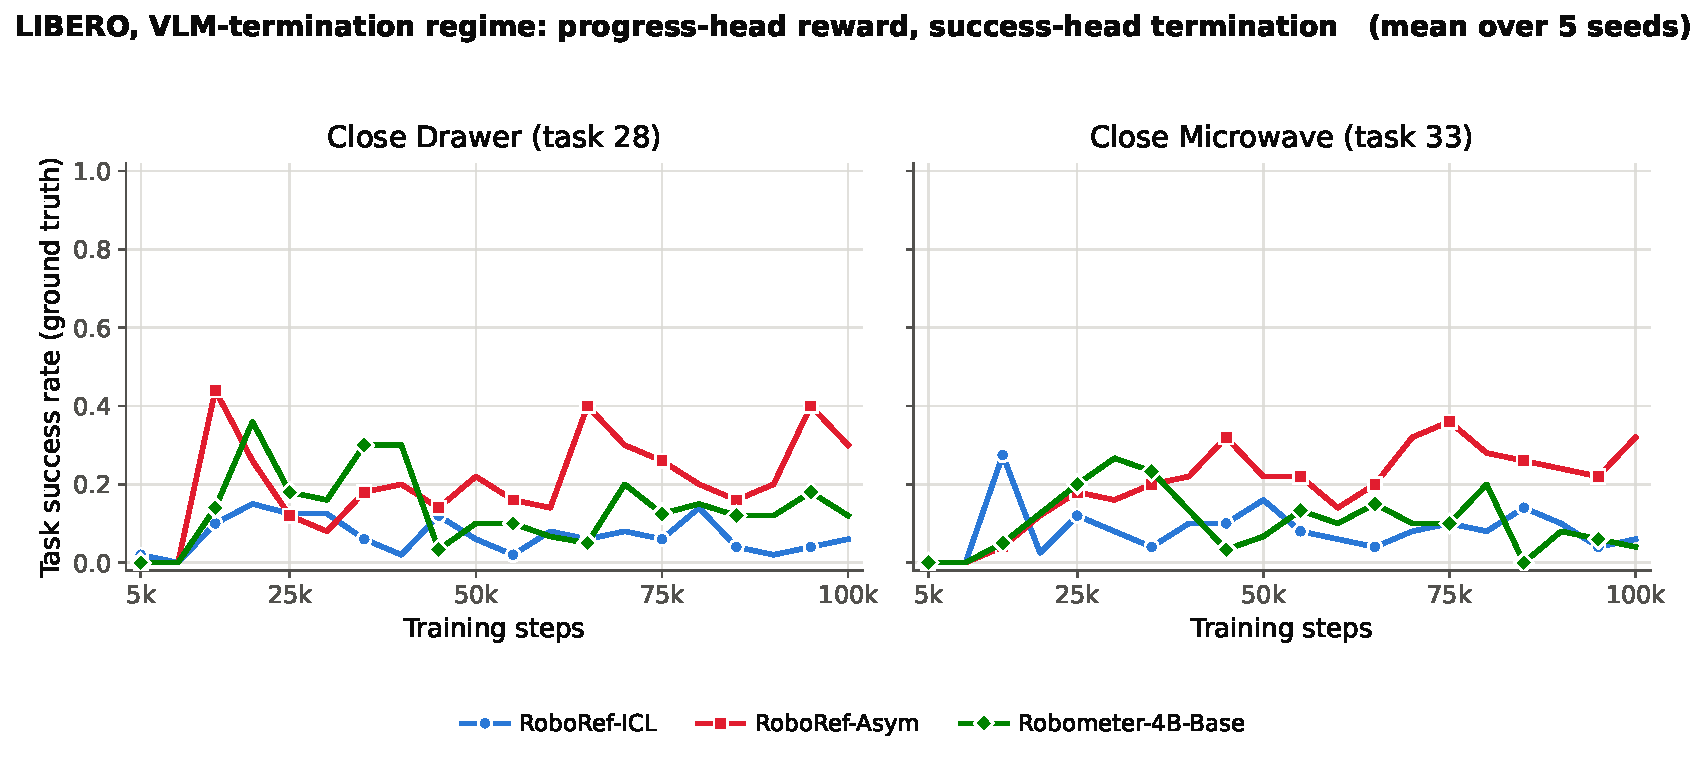
\includegraphics[width=\textwidth]{media/results/libero_termination_rl.pdf}
\caption[LIBERO under the progress-head deployment regime]{The progress heads compared under Robometer's own deployment regime, a dense progress reward with success-head termination, five seeds per model. RoboRef-Asym holds the upper hand on both tasks, as it does on MetaWorld, but no model trains either task well, with every curve peaking below $0.5$.}
\label{fig:libero-termination}
\end{figure*}



LIBERO is the benchmark Robometer itself reports downstream results on, so it is the one place a direct comparison against the released model on its own ground is possible. One property of the setup should be stated before any curve is read. LIBERO-90 is part of Robometer's released training corpus, so our fine-tunes, trained on our re-curation of that corpus, have seen this benchmark during training, while the released Robometer-4B checkpoint predates its inclusion and has not. Its training corpus does include the other LIBERO suites, so the benchmark is still in-distribution for the baseline as well. The comparison is therefore not entirely fair, and the direction of the unfairness runs in our favour, which frames how the results below should be weighed.

We train on two LIBERO-90 tasks, Close-Drawer and Close-Microwave, five seeds per reward model for one hundred thousand steps, and as everywhere else we score each seed by ground-truth task success measured where the reward model is never queried. The setup of Section~\ref{sec:results-rl-config} carries over with one exception. The released Robometer-4B runs here in the dense progress regime with no termination signal, not the sparse detector form it used on MetaWorld, because the dense form is its best configuration on this benchmark and our success rate figures report each model at its best. Our models run the sparse success-head protocol with per-model calibrated thresholds, $0.85$ and $0.80$ on the two tasks for RoboRef-Asym and $0.86$ for RoboRef-ICL, all inside the range the calibration discussion anticipated. The minimum episode length sits at $80\%$ of the demonstration length, where the demonstrations average two hundred steps.

Figure~\ref{fig:libero-rl} shows the comparison at each model's best configuration. Close-Drawer is the one downstream task in this thesis where the released baseline finishes above our models, which comes as a surprise, since the training data would predict the opposite, our fine-tunes have seen LIBERO-90 and the released checkpoint has not. Under its dense, non-terminating form the baseline climbs for the whole run and ends at perfect success. This is the baseline's best showing on any benchmark, and is very different from the rest of its own record, near zero on MetaWorld under every configuration we tried. Our sparse fine-tunes land in the band below it, RoboRef-Asym around $0.65$ late in training and RoboRef-ICL near $0.5$ at its peak, with RoboRef-Std, LRM, RoboDopamine, and RoboReward moving between transient peaks and slow decay. Close-Microwave resists everyone. No reward model, ours or published, trains a policy past $0.35$, and most are well under it, which makes the task less a ranking of models than a shared ceiling on what these rewards can currently teach.

Then, we add one more comparison. Every downstream result of ours so far, on MetaWorld and on LIBERO, reads the success head, so the progress head, the head Robometer's own paper deploys, has not yet driven a policy anywhere in this thesis. Figure~\ref{fig:libero-termination} runs exactly that comparison, our two deployment models against the released baseline, all three under a dense progress-head reward with success-head termination, the exact deployment regime of the Robometer paper. The reward is the per-step progress value, an episode ends when the success head crosses the model's threshold, and the minimum-length rule above still holds.

\begin{figure*}[t]
\centering
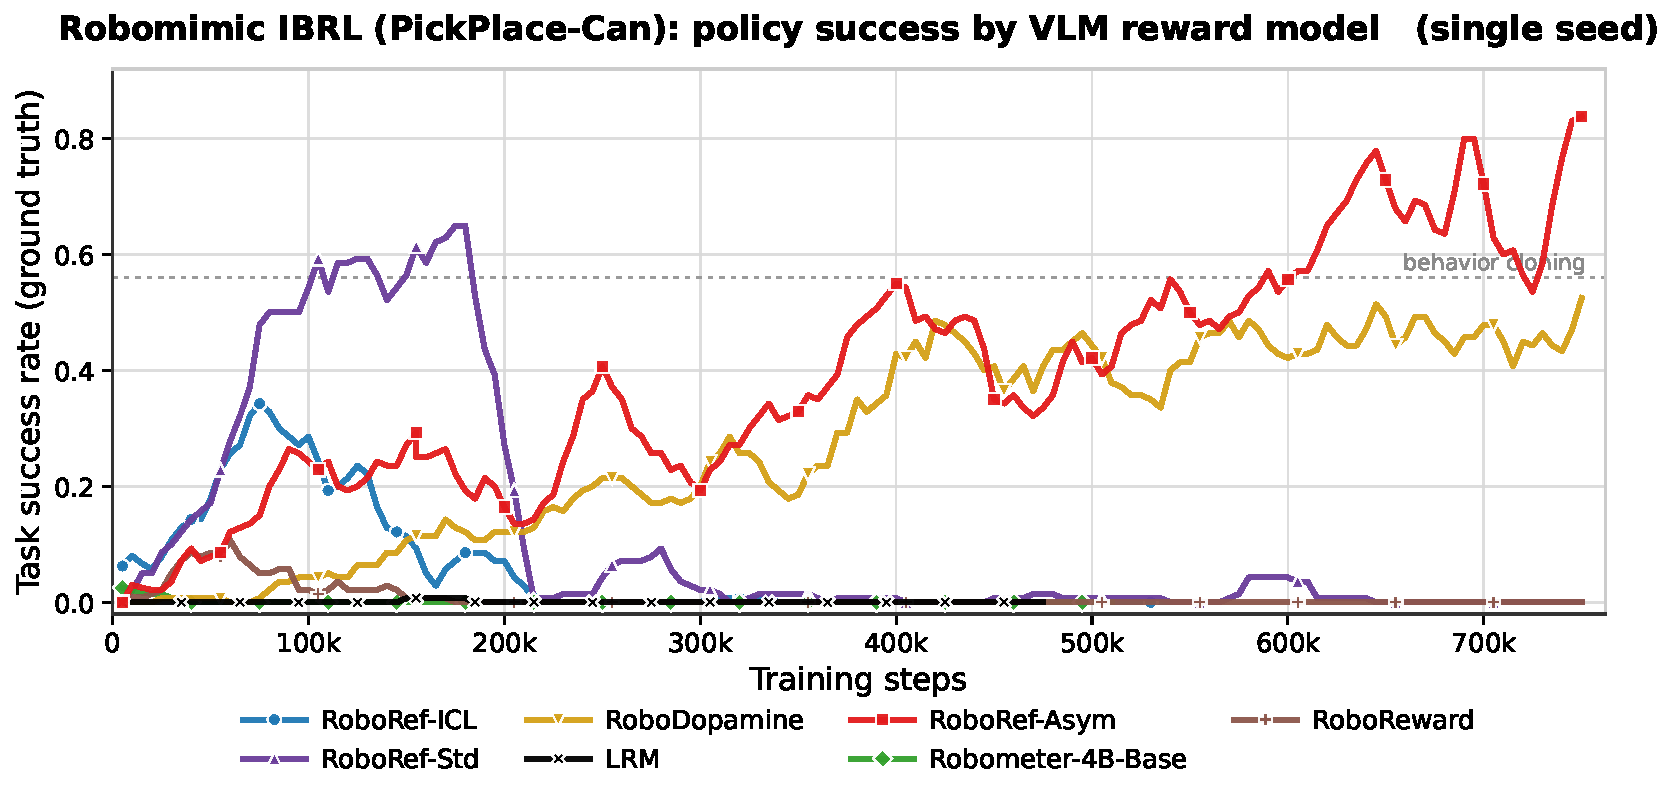
\includegraphics[width=0.72\textwidth]{media/results/robomimic_rl.pdf}
\caption[Robomimic downstream reinforcement learning]{Robomimic downstream reinforcement learning on PickPlace-Can, a domain absent from every reward model's training data, one seed per reward model, smoothed ground-truth success over $750$k training steps. The dashed line marks the behavior-cloning policy that IBRL starts from, at a success rate of $0.56$. Each reward runs in its Table~\ref{tab:rl-config} configuration. RoboRef-Asym is the only reward that ends above the cloning line, at $0.84$ and still climbing; RoboDopamine recovers the demonstrations' competence without exceeding it; RoboRef-Std and RoboRef-ICL rise early and collapse; everything else stays at the floor.}
\label{fig:robomimic-rl}
\end{figure*}

The three models are comparable across both tasks, RoboRef-Asym holds the upper hand for most of training on both, echoing its MetaWorld standing, and the released baseline stays within reach of it, closer than anywhere else in our downstream results. At the same time nothing here approaches the sparse-protocol numbers, every curve on both tasks peaks below $0.5$, and neither task can be called well trained under this regime. 

This result shows two things. First, the released Robometer-4B is weaker than its paper suggests, since in the paper's own configuration it fails to train a good policy on either task. In their figure, however, the model was further trained with LoRA on LIBERO tasks, which apparently was necessary to get good performance. Second, under the regime these models are most naturally built for, a dense reward that leverages the dense labels while the success head closes the episode, none of the models succeeds, ours included.

\subsection{Robomimic}
\label{sec:results-rl-robomimic}

Robomimic is the last benchmark of this evaluation. No reward model in this comparison, ours or the published ones, ever trained on its scenes or its rendering, so every reward is judging a world it has never seen. The task is PickPlace-Can, lifting a can out of one bin and placing it into another. The setup of Section~\ref{sec:results-rl-config} carries over, our models again reading the success head as a sparse reward, with two practical differences. Robomimic steps far more slowly than the other simulators, so a $750$k-step run takes several days and we report a single seed per reward model, spending the compute budget on covering models, not repetitions. And the minimum episode length sits at the full demonstration length of $120$ steps in comparison to the $80\%$ MetaWorld used, because at the lower setting the familiar failure pattern returned, success signals fired before the task was physically solvable and the policies began farming them.

The results can be seen in Figure~\ref{fig:robomimic-rl}. Because IBRL starts from the behavior-cloning policy, the dashed line at $0.56$ is the bar that matters, and any curve that ends above it has learned something the demonstrations alone could not teach. One reward clears it. RoboRef-Asym climbs for essentially the whole run, passes the cloning line for good near $590$k steps, and is still rising at $0.84$ when the budget ends. This is the result we most wanted from this benchmark. On a domain that is fully out of distribution for the reward model, the conservative fine-tune carried an RL policy well past the demonstrations it started from.

Among the baselines, RoboDopamine is the only one that trains a real policy, climbing steadily to $0.53$. It earns the credit for that, and it still ends just below the cloning line, so it recovers the competence already in the demonstrations without moving beyond it. RoboReward and LRM never leave the floor, while Robometer-4B, back in its sparse detector form after its dense LIBERO run, returns to a flat performance like MetaWorld.

In addition, RoboRef-Std is the fastest starter in the figure, above the cloning line within roughly $105$k steps and peaking at $0.65$. Its only differences from the released Robometer-4B, flat at zero for the entire run, are our training data and the dropped preference head, so this early stretch is RQ1, the failure-data question, measured on-policy. The failure supervision alone turns a reward that never moves a policy on this domain into one that drives genuine learning for its first two hundred thousand steps, clearing the cloning line at its peak. 

What the data cannot do alone is hold the gain. The observation comes first. RoboRef-Std falls from its peak to zero in the space of a few evaluations and never returns, and RoboRef-ICL, after an early rise to $0.34$, comes apart at the same point of training. We have no ground-truth count of false positives on Robomimic to prove the mechanism, but the pattern matches the one MetaWorld made visible, a policy that eventually finds false positives the symmetric loss left standing, and the fine-tune trained with the asymmetric objective on the same data is the one that does not collapse. The offline numbers pointed the other way. On the out-of-distribution table, RoboRef-ICL was the best of our fine-tunes at the strict false-positive budget (Table~\ref{tab:offline-ood}), yet on-policy it is RoboRef-Asym that survives. A single seed warrants some caution about the exact numbers, but the margin between a policy at $0.84$ and a field that ends below the cloning line is not the kind noise produces.

\section{What the downstream results add up to}
\label{sec:results-rl-summary}

MetaWorld and Robomimic sit at opposite ends of the distribution shift the reward models face, one a domain where our training data gives us a clear edge, the other a domain nobody trained on. They return the same verdict. The rewards that train competent policies are the asymmetric fine-tunes, RoboRef-Asym everywhere and RoboRef-ICL where the domain is familiar, while the released baseline and the three published reward models either sit silent at the floor or, at best, give back the competence the demonstrations already contained. The division of labor between our contributions is visible in the curves themselves. The failure data supplies the discriminative signal, which is why RoboRef-Std rises on Robomimic where the released model never moves, and the asymmetric loss is what lets a model keep what the data taught it.

LIBERO sits between those two ends and complicates the verdict in an instructive way. It is the one benchmark where the released baseline posts a genuine win, perfect success on Close-Drawer under its dense, non-terminating form, and the one task nobody trains, Close-Microwave, caps every reward model at $0.35$. The regime study of Figure~\ref{fig:libero-termination} supplies the sharper reading. Under the deployment form its own paper reports, dense progress with success-head termination, the released model trains neither task well, and our fine-tunes, while ahead of it there too, do not convert their offline edge into strong policies either. The benchmark that should have been the baseline's home ground ends up showing that the deployment regime, as much as the model, decides what these rewards can teach. The same study is candid about our own models. The progress head remains their least developed part, since it never produced clear downstream gains in any of our experiments, a limitation the next chapter takes up.

Almost none of this was visible offline, and that is the answer to RQ4, which asked whether offline reward-quality gains transfer to downstream reinforcement learning. The released Robometer-4B reproduces the offline numbers of its own paper and never trains a policy. RoboRef-Std matches the asymmetric models on nearly every offline column and collapses in MetaWorld and Robomimic. The out-of-distribution table ranks RoboRef-ICL above RoboRef-Asym at the strict operating point, and on-policy the order flips. Offline evaluation scores a reward on a fixed set of trajectories, but an optimizing policy is not a fixed set; it is a search process that actively hunts for the inputs the reward gets wrong, and it finds them. The one offline quantity that pointed in the right direction was class separation at the conservative operating point, where the asymmetric loss stood out, and even that only hinted at the size of the on-policy gap. Offline reward-quality gains transfer only when they come packaged with conservatism, and when they do not transfer, the mechanism is the one Figure~\ref{fig:mw-reward} makes visible, a policy farming the reward's false positives. The next chapter takes up what this means beyond our own models.

        \chapter{Discussion}
\label{sec:discussion}

The previous chapter ended on a gap, reward models that look strong on every standard offline metric and still fail the moment a policy optimizes against them. This chapter places that finding, and our results more broadly, against the prior work, then takes an honest inventory of what limits them and what they imply beyond this thesis.

\section{Reading the results against prior work}

Our results do not contradict the published claims of the models we compare against. Robometer reports strong offline reward quality and real-world RL with its released model, and our evaluation reproduces its offline numbers on the held-out-robot set, which is what lets us trust the rest of our harness. What Robometer never reports is the experiment at the center of this thesis, the released model driving simulated RL without in-domain adaptation, and in that experiment it fails on almost every task we test. The same holds down the table. RoboReward was only ever validated in the real world, RoboDopamine adapts to each task from a demonstration before learning, and LRM, the one prior model tested zero-shot in simulated RL, pays our policies the richest reward in the comparison while producing almost no success. Each system behaves as its paper says it does. The problem is that the evaluations those papers chose did not surface the failure mode that dominates once a policy is in the loop.

One could ask whether our results reflect a plain real-to-sim gap, models that simply cannot read simulated frames. We doubt that this is the main source. These models already train on simulated data, Robometer's corpus includes the LIBERO suites and MetaWorld clips among its sources, and the released model's perfect Close-Drawer run shows it can score simulated frames well enough to train a policy to full success when the regime suits it. A rendering gap may contribute at the margin, but the failure mode we observe, reward paid rising while true success stays flat, is exploitation, not blindness. The simulated setting also has a virtue beyond ground truth. Real-world experiments are hard to reproduce, while simulated ones can be rerun exactly, so we would encourage future reward models to be tested thoroughly in simulation as well, where such claims can be checked by anyone.

That failure mode is not new in kind. Learned reward functions have been known to invite exploitation since the early safety literature \citep{amodei_concrete_2016}, and reinforcement learning from human feedback showed that optimizing a policy against a learned proxy eventually degrades true performance even as the proxy climbs \citep{gao_scaling_2023}. What our experiments add is a concrete robotic instance in which the mechanism is directly observable, because simulation provides ground-truth success independent of the reward. The paired curves of Figure~\ref{fig:mw-reward}, reward paid rising while true success stays at zero, are overoptimization made visible, and we would argue that reporting this pair should become standard practice for reward-model papers, since either curve alone tells a misleading story.

Our asymmetric objective, in turn, is the training-time counterpart of an observation made at inference time by \citet{gumbsch_demonstrations_2026}, that false positives mislead an optimizing policy far more than false negatives. Building that asymmetry into the loss is what separates the surviving fine-tunes from the collapsing ones in both simulators, and it costs almost nothing to adopt, a reweighting of an existing objective that resumes directly from pretrained weights.

It is worth spelling out why these two ingredients help, because the mechanism carries beyond our models. A corpus of successful demonstrations teaches a reward what completed tasks look like, but a policy in training spends nearly all of its time in states no demonstration contains, half-finished reaches, near-misses, and outright failures, and on those states a success-trained model is free to guess, usually upward. Our failure data fills exactly the region the policy actually visits, which is why the data alone lifts a reward from never moving a policy on Robomimic to training one. The asymmetric loss adds the complementary piece. The most dangerous residual errors are the near-misses that look almost complete, and pricing false positives above false negatives pushes precisely those below the firing threshold. The data covers the states an optimizing policy reaches, the loss decides how to err on them, and it is the combination that survives optimization.

The dense progress labels have to pass the same test. Offline they deliver, and the ablation of Section~\ref{sec:results-icl} ties those gains to the data they came from, but as a live reward the progress head never made its case, a shortfall we return to with the limitations below.

\section{Why the offline metrics missed it}

Offline evaluation scores a reward on trajectories drawn from a fixed distribution. A policy under training is not such a distribution. It is a search process that shifts probability toward whatever the reward scores highly, so a region of false positives that occupies a negligible slice of a test set becomes, once discovered, most of what the reward is asked to judge. The shift is not even neutral. For overestimated states reinforcement learning is adversarial to the reward model, since every error the policy discovers is revisited, trained on, and exploited harder, a feedback loop that self-amplifies exactly the mistakes a fixed test set touches only once. Metrics that integrate over the whole score range, ROC-AUC above all, are close to blind to this, because they average over operating points a deployed detector will never use. The quantities that came closest to predicting our downstream results were the ones tied to a conservative operating point, the true-positive rate at a strict false-positive budget and the class separation $d'$, and even these were only necessary signals, not sufficient ones. RoboRef-Std posted a respectable $d'$ of $1.08$ and still came apart under an optimizing policy. We looked for an offline number that cleanly forecasts on-policy survival and did not find one, which is itself a result: with the metrics the field currently reports, the downstream test cannot be skipped.

\section{Limitations}

The claim we can defend is direction, not finality. We identified the dominant failure mode of current vision-language reward models, built a dataset, an input format, and an objective that target it, and the resulting models beat every published reward model we tested in most of the RL regimes we evaluate. What we cannot claim is stability. A reward model's behavior shifts with the checkpoint and the threshold it is read at, off-policy actor-critic methods are notoriously sensitive on their own, and the two sensitivities compound, so individual runs can and do surprise, as the early rise and collapse of two of our own fine-tunes on Robomimic shows. This bears on the reliability of any single curve we report, and it is compounded by seed counts that are honest for a compute-bound academic project but modest by RL standards, five per model on MetaWorld and LIBERO and a single seed on Robomimic, where one run takes several days.

The second limitation is scope, and for a robotics thesis it is the one that matters most: every policy we train lives in simulation. Simulation is what makes the ground-truth success measurements behind our central finding possible at all, but a real robot adds shifting lighting, changing scenes, sensor noise, and no simulator state to calibrate against, and our only evidence about real-world behavior is offline, the held-out-robot evaluation set. The generalizability of the downstream results to physical hardware is therefore untested, and claiming otherwise would repeat exactly the evaluation gap we criticize in prior work.

A further limitation sits inside the dataset contribution itself. The per-frame progress labels are the most expensive part of our corpus, and while the offline chapters justify them, the configuration that trains the best policy reads the success head as a sparse detector in every benchmark. MetaWorld and Robomimic therefore report no progress-head runs, and in the LIBERO regime study, the one place the progress head is deployed as the reward, our models improve on the baseline yet do not train the tasks to a strong success rate. The evidence that the dense labels help downstream is indirect, running through the success head that was trained alongside them, and a policy driven by the progress signal itself is something this thesis does not validate.

Our deployment recipe is also not fully zero-shot. The success threshold is calibrated per model on a small set of rollouts, and although we found the working range to be narrow and stable, between $0.75$ and $0.90$ across simulators and tasks, the procedure still needs some calibration. The minimum episode length is the other per-task number, and it mattered for every vision-language reward model in the comparison, not only ours. It is also easy to set. The length of a demonstration worked in every simulator, and those demonstrations were already there, since IBRL pretrains its policy on them. Outside the in-context model we take no images and no actions from them, only a single number. One can still object that needing that number makes the method less than strictly zero-shot, and the objection is fair, though the same could be said of the maximum episode length that every policy setup fixes per task without anyone counting it as supervision. The next natural step is to move the threshold calibration online, adjusting it from the policy's own behavior during training, and to search for general minimum-length values that hold across a whole suite instead of per task.

\section{Ethical considerations}

Three concerns are worth naming. The first is safety. A reward model that fires falsely on a real robot does not just corrupt a learning curve, it reinforces physical behavior that never achieved the task, and an optimizing policy will repeat whatever was reinforced. Conservatism is therefore not only a performance choice but the safety-aligned default for any learned reward that touches hardware, and we see our results as evidence for making it standard. The second concern is inherited bias. These reward models judge the physical world through backbones pretrained on internet data, and whatever blind spots that data carries, scenes, objects, and environments it underrepresents, propagate silently into which robot behaviors get rewarded. The third is oversight. Our labeling pipeline replaces human annotation with large models precisely because the corpus is too large to label by hand, which also means no human ever verifies most of the labels the reward model learns from. We audited samples and measured error rates, but automated curation at this scale trades away a layer of human review, and that trade should be stated, not hidden. Alongside these concerns sits the compute cost of the whole enterprise, from labeling a million clips with large models to fine-tuning on H100 nodes, an energy footprint that grows with every scaling step the field takes.

The limitations above sketch the road ahead, a real-world reinforcement learning loop as the decisive test, online threshold calibration to close the zero-shot gap, and reward pretraining for newer backbones.

        \chapter{Conclusion}
\label{sec:conclusion}

This thesis started from a gap in how vision-language reward models are evaluated. The field reports strong offline metrics and selected reinforcement learning results, real-world runs or simulated runs after in-domain adaptation, and the most intuitive experiment, a released foundation reward model driving simulated RL as it stands, was missing. We built RoboRef for exactly that test, a reward model meant to perform well while a policy optimizes against it, through a re-curated corpus whose failures carry dense per-frame progress labels, an optional in-context demonstration alongside every query, and an asymmetric objective that makes false positives the expensive mistake. The work was organized around four short questions. Can a reward model trained mostly on successful demonstrations handle the failures a policy generates, or is failure data needed (RQ1)? Do in-context demonstrations improve its judgment (RQ2)? Are these models overconfident, and does an asymmetric loss make them harder to exploit (RQ3)? And do offline gains transfer to downstream reinforcement learning (RQ4)? We can now answer each in turn.

\textbf{RQ1}, whether failure supervision improves the discrimination of success from failure, has a clear answer in distribution. Changing nothing but the training data lifts rank accuracy from $0.611$ to $0.771$ and doubles the true-positive rate at a strict false-positive budget. The ablation of Section~\ref{sec:results-icl} answers the question exactly from the other side, since continuing to train the released model with our loss but on its own data moves rank accuracy only from $0.61$ to $0.64$, against the $0.85$ the same loss reaches with our corpus, so the gain belongs to the failure data and not to the objective wrapped around it. On Robomimic the standard-loss fine-tune, which differs from the released model in the training data alone, clears behavior cloning on a domain where the released model never moves at all, the data's contribution measured on-policy. That it cannot hold the gain without the asymmetric loss makes the division of labor plain. The data is the foundation the other two contributions stand on, necessary even where it is not sufficient. However, it should be noted that the best RL results come from the success head, which the dense per-frame labels do not directly supervise. Whether the reason behind this is the training loss of the progress head or our per-frame labeled dataset remains an open question.

\textbf{RQ2}, whether in-context demonstrations improve the model's judgment, has to be answered by the standard this thesis has insisted on. Offline the demonstration is the clearest yes we measured. It lifts rank accuracy to $0.896$, more than $27$ points above the released baseline, with the widest and still-growing margin on the real-world split, exactly where a textual task description is thinnest. We have argued throughout, however, that offline metrics are not where a reward model earns its keep, and on-policy the case does not hold. Across MetaWorld, LIBERO, and Robomimic the ICL variant is never clearly better than the plain asymmetric fine-tune, while the demonstration doubles the input the model reads on every query and with it the cost of deployment. By our own standard the answer is therefore negative. The demonstration sharpens judgment on a fixed test set but does not buy a better policy, and at twice the inference cost it is not justified in the loop as we deployed it. That the largest offline gain in the thesis does not survive the optimizing policy already previews the answer to RQ4.

\textbf{RQ3} asked whether these models are overconfident and whether an asymmetric loss makes them harder to exploit. Both halves held. The released baseline scores genuine failures next to genuine successes and, under an optimizing policy, pays out the most reward in the comparison while training a policy that never succeeds. The asymmetric loss is the single largest downstream factor we measured, the whole distance between a fine-tune that collapses under an optimizing policy and one that reaches $0.72$ on MetaWorld and ends above behavior cloning on a domain it never saw.

\textbf{RQ4}, whether offline gains transfer to downstream RL, gets the answer no, not by themselves, and this is the finding we consider most important beyond our own models. Offline metrics score a fixed distribution while a policy actively searches for the reward's mistakes, so a model can match the best fine-tunes on nearly every offline column and still be pulled apart on-policy. What transfers is conservatism. The failure mechanism, visible because simulation provides ground truth, is a policy farming false positives, collecting reward that rises while true success does not.

The main question, to what extent a fine-tuned vision-language model can serve as a usable and generalizable reward for robot RL, therefore gets a conditional but genuinely positive answer. With failure supervision and a conservative objective, one reward model trained policies across every simulated domain we tested, including one fully outside its training distribution, and delivered the strongest overall downstream record of any reward model in the comparison. 

However, deployment needs a calibrated threshold and one demonstration-length prior, results inherit the sensitivity of both the model and the RL algorithm beneath it, and everything we show lives in simulation, with seed counts bounded by compute. A real-world learning loop, online threshold calibration, and reward pretraining on newer backbones are where this work should go next. What the thesis establishes is the direction: a foundation reward model earns that name in the RL loop, not on a leaderboard, and the way to survive the loop is to make the reward hard to exploit.


\bibliographystyle{ACM-Reference-Format}
\bibliography{bibliographies/references_filtered}

% \newpage
\appendix
        % Appendix is one-column so the wide dataset tables and the figure gallery have room.
\onecolumn

\chapter{The RBM-1M Dataset}
\label{apx:rbm1m}

RBM-1M is the corpus RoboRef re-curates, the training set behind Robometer \citep{robometer}. Table~\ref{tab:rbm1m} gives its composition from our scan of the released archives, one row per major source, grouped by embodiment. That grouping is the one that drives the re-curation. The standard robot arms are the manipulation data our work centers on, and they hold every failure in the corpus. The humanoid and human-only groups are large and broaden the visual coverage, but sit away from the single-arm setting our downstream tasks use, which is why we hold them out of the shared training corpus. A selection of them, listed in Appendix~\ref{apx:roboref-data}, is used once, in the first training phase of the Qwen3.5 model (Section~\ref{sec:method-dataset}).

\begin{table}[h]
\centering\footnotesize
\caption[Composition of RBM-1M]{Composition of RBM-1M, the corpus RoboRef re-curates, from a scan of Robometer's released archives. Sources are grouped by embodiment, and only the standard robot arms carry failures. Counts are archive-level entries, one row per camera view; the text explains why they run ahead of the number of distinct trajectories.}
\label{tab:rbm1m}
\begin{tabular}{@{}p{6.6cm}rrr@{}}
\toprule
Source & Failures & Successes & Total \\
\midrule
\multicolumn{4}{@{}l}{\emph{Humanoid}}\\
AgiBot \citep{agibot-world-contributors_agibot_2025} & 0 & 433{,}821 & 433{,}821 \\
Galaxea \citep{jiang_galaxea_2025} & 0 & 108{,}118 & 108{,}118 \\
Humanoid Everyday \citep{zhao_humanoid_2025} & 0 & 9{,}208 & 9{,}208 \\
\quad Subtotal & 0 & 551{,}147 & 551{,}147 \\
\addlinespace
\multicolumn{4}{@{}l}{\emph{Human-only (hand)}}\\
EgoDex \citep{hoque_egodex_2025} & 0 & 313{,}109 & 313{,}109 \\
EPIC \citep{damen_scaling_2018} & 0 & 37{,}030 & 37{,}030 \\
RH20T, human \citep{fang_rh20t_2024} & 0 & 14{,}225 & 14{,}225 \\
H2R & 0 & 2{,}254 & 2{,}254 \\
Other human-hand archives & 0 & 81 & 81 \\
\quad Subtotal & 0 & 366{,}699 & 366{,}699 \\
\addlinespace
\multicolumn{4}{@{}l}{\emph{Standard robot arms}}\\
DROID \citep{khazatsky_droid_2024} & 0 & 149{,}804 & 149{,}804 \\
RT-1 (Fractal) \citep{oneill_open_2024} & 0 & 87{,}204 & 87{,}204 \\
Bridge V2 \citep{oneill_open_2024} & 0 & 83{,}024 & 83{,}024 \\
Language Table \citep{oneill_open_2024} & 0 & 50{,}000 & 50{,}000 \\
BC-Z \citep{oneill_open_2024} & 0 & 43{,}261 & 43{,}261 \\
RoboSet \citep{oneill_open_2024} & 0 & 36{,}480 & 36{,}480 \\
RH20T \citep{fang_rh20t_2024} & 0 & 15{,}744 & 15{,}744 \\
MolmoAct \citep{lee_molmoact_2025} & 0 & 15{,}546 & 15{,}546 \\
FailSafe \citep{lin_failsafe_2025} & 58{,}153 & 13{,}461 & 71{,}614 \\
RoboReward \citep{roboreward} & 88{,}418 & 19{,}852 & 108{,}270 \\
RACER \citep{dai_racer_2025} & 29{,}211 & 7{,}131 & 36{,}342 \\
RoboArena \citep{atreya_roboarena_2025} & 17{,}510 & 2{,}635 & 20{,}145 \\
SOAR \citep{zhou_autonomous_2024} & 12{,}009 & 4{,}803 & 16{,}812 \\
LIBERO \citep{liu_libero_2023} & 6{,}241 & 5{,}659 & 11{,}900 \\
AutoEval \citep{zhou_autoeval_2025} & 3{,}721 & 4{,}956 & 8{,}677 \\
Furniture Bench \citep{heo_furniturebench_2023} & 0 & 5{,}100 & 5{,}100 \\
MetaWorld (ReWiND) \citep{zhang_rewind_2025} & 0 & 100 & 100 \\
Other standard-arm archives & 274 & 13{,}716 & 13{,}990 \\
\quad Subtotal & 215{,}537 & 558{,}476 & 774{,}013 \\
\midrule
Total & 215{,}537 & 1{,}476{,}322 & 1{,}691{,}859 \\
\bottomrule
\end{tabular}
\end{table}

The counts are archive-level entries, not distinct trajectories. Several sources are expanded across camera views, the long-horizon humanoid data across annotated sub-steps, and RoboReward is stored at two resolutions, so these figures run ahead of the number of unique recorded attempts. AgiBot is the clearest case of the first, about $34{,}000$ long-horizon trajectories appearing as $216{,}911$ sub-step entries under each of two camera archives, and the RoboReward archives hold every clip twice, once per resolution. This expansion, together with the re-curation of Section~\ref{sec:method-dataset}, is why RBM-1M counts well over a million entries here while our re-curated standard-arm corpus holds $648{,}714$ rows. The same two effects also explain why our per-source counts do not line up with Robometer's published Table~IX. We count one row per scored clip, an episode from a single camera view, while Robometer counts every unique video-language annotation expanded across views, so we report our own episode-level numbers throughout and do not attempt a row-by-row reconciliation. The 100 MetaWorld demonstrations listed are ReWiND's, the only MetaWorld in RBM-1M; our re-curation drops them in favor of the MetaWorld data we generate ourselves (Section~\ref{sec:method-dataset}).

\chapter{The RoboRef Dataset}
\label{apx:roboref-data}

This appendix expands the summary of Section~\ref{sec:method-dataset}. Table~\ref{tab:roboref-dataset} there reports the composition at the level the main text needs. Here we break the same corpus down to one row per upstream source, say where each failure label comes from, and give the pairing and sampling details the training pipeline relies on. Unless noted, every count below describes the standard-arm corpus that all six models share, $648{,}714$ rows, where one row is one episode rendered from a single camera view. The humanoid and human-only pool that only the Qwen3.5 first phase uses is made of successes alone, and we return to it at the end of the first section.

\section{Per-source composition}

Table~\ref{tab:roboref-detailed} gives the full per-source composition, one row per major upstream source, in the style of Robometer's own dataset table. Its upper three blocks are the standard-arm corpus that every model trains on. The retained expert demonstrations are the largest part and come almost entirely from Open X-Embodiment sources \citep{oneill_open_2024} carried over from RBM-1M, with DROID, RT-1 and Bridge the three biggest. The retained mixed-expertise archives are the smaller corpora that actually carry failures, chief among them RACER, RoboArena and SOAR. Below them sit the sources we add or replace ourselves. Set apart at the foot of the table is the humanoid and human-only pool, which only the Qwen3.5 model sees, in its first phase alone.

\begin{table}[h]
\centering\footnotesize
\caption[Per-source composition of the RoboRef dataset]{Full per-source composition of the RoboRef dataset, one row per major upstream source, after the style of Robometer's Table~IX. The upper three blocks form the standard-arm corpus that all six models share; the final block is the humanoid and human-only pool used only for the Qwen3.5 first phase. Counts are episodes, one row per camera view. Expert-demonstration sources are success-only, and small sources are gathered into ``other'' rows. Totals match Table~\ref{tab:roboref-dataset}.}
\label{tab:roboref-detailed}
\begin{tabular}{@{}p{6.6cm}rrr@{}}
\toprule
Source & Failures & Successes & Total \\
\midrule
\multicolumn{4}{@{}l}{\emph{Expert demonstrations retained from RBM-1M}}\\
DROID \citep{khazatsky_droid_2024} & 0 & 149{,}804 & 149{,}804 \\
RT-1 (Fractal) \citep{oneill_open_2024} & 0 & 87{,}204 & 87{,}204 \\
Bridge V2 \citep{oneill_open_2024} & 0 & 83{,}023 & 83{,}023 \\
Language Table \citep{oneill_open_2024} & 0 & 50{,}000 & 50{,}000 \\
BC-Z \citep{oneill_open_2024} & 0 & 39{,}344 & 39{,}344 \\
RoboSet \citep{oneill_open_2024} & 0 & 36{,}480 & 36{,}480 \\
RH20T \citep{fang_rh20t_2024} & 0 & 15{,}744 & 15{,}744 \\
MolmoAct \citep{lee_molmoact_2025} & 0 & 15{,}324 & 15{,}324 \\
Other Open X-Embodiment archives \citep{oneill_open_2024} & 0 & 13{,}875 & 13{,}875 \\
\addlinespace
\multicolumn{4}{@{}l}{\emph{Mixed-expertise archives retained from RBM-1M}}\\
RACER \citep{dai_racer_2025} & 29{,}211 & 7{,}131 & 36{,}342 \\
RoboArena \citep{atreya_roboarena_2025} & 17{,}510 & 2{,}635 & 20{,}145 \\
SOAR \citep{zhou_autonomous_2024} & 11{,}999 & 4{,}797 & 16{,}796 \\
LIBERO \citep{liu_libero_2023} & 6{,}241 & 5{,}659 & 11{,}900 \\
AutoEval \citep{zhou_autoeval_2025} & 3{,}721 & 4{,}946 & 8{,}667 \\
Other retained archives & 241 & 861 & 1{,}102 \\
\addlinespace
\multicolumn{4}{@{}l}{\emph{Added or replaced by us}}\\
MetaWorld \citep{yu_meta-world_2019} (added, simulator) & 24{,}402 & 1{,}850 & 26{,}252 \\
RoboReward partials \citep{roboreward} (replaced) & 15{,}860 & 7{,}313 & 23{,}173 \\
DROID failures (added) & 5{,}503 & 5{,}863 & 11{,}366 \\
FailSafe \citep{lin_failsafe_2025} (replaced, simulator) & 2{,}098 & 75 & 2{,}173 \\
\midrule
Standard-arm total & 116{,}786 & 531{,}928 & 648{,}714 \\
\midrule
\multicolumn{4}{@{}l}{\emph{Phase-1 pretraining only (Qwen3.5 first phase)}}\\
Galaxea \citep{jiang_galaxea_2025} (humanoid) & 0 & 103{,}421 & 103{,}421 \\
Humanoid Everyday \citep{zhao_humanoid_2025} (humanoid) & 0 & 9{,}208 & 9{,}208 \\
EgoDex \citep{hoque_egodex_2025} (human hand) & 0 & 48{,}447 & 48{,}447 \\
EPIC \citep{damen_scaling_2018} (human hand) & 0 & 37{,}030 & 37{,}030 \\
RH20T, human \citep{fang_rh20t_2024} (human hand) & 0 & 13{,}986 & 13{,}986 \\
Other human-hand archives & 0 & 2{,}335 & 2{,}335 \\
\midrule
Total with phase-1 data & 116{,}786 & 746{,}355 & 863{,}141 \\
\bottomrule
\end{tabular}
\end{table}

The block at the foot of the table, Galaxea and Humanoid Everyday on the humanoid side and EgoDex, EPIC and RH20T on the human-hand side, is kept apart. These trajectories are successes only, labeled like other successes by the $t/T$ heuristic, so they add no failures and leave the label and pairing breakdowns below unchanged. Only the Qwen3.5 model uses them, and only in its first phase, where its cold reward heads gain from the broader visual coverage before the second phase narrows to the standard-arm corpus that all six models share. Every other count in this appendix describes that standard-arm corpus of $648{,}714$ rows.

\section{Where the labels come from}

Every successful trajectory in the dataset, whatever its source, is labeled by Robometer's $t/T$ progress heuristic, the cheap monotone ramp of Section~\ref{sec:method-dataset}, so all $531{,}928$ successes share one labeling route. The failures are where the work is, and their $116{,}786$ labels come from three different routes depending on where the failure was produced. Table~\ref{tab:roboref-labels} gives the split.

\begin{table}[h]
\centering\footnotesize
\caption[Sources of the failure labels]{Origin of dense per-frame failure labels. Successes are omitted, since all $531{,}928$ of them use Robometer's $t/T$ heuristic.}
\label{tab:roboref-labels}
\begin{tabular}{@{}p{4.0cm}p{6.0cm}r@{}}
\toprule
Label route & Sources & Failures \\
\midrule
Simulator ground truth & MetaWorld, FailSafe & 26{,}500 \\
VLM+LLM pipeline & DROID, RACER, RoboArena, SOAR, LIBERO, AutoEval, and the other retained archives & 74{,}426 \\
Ramp to clip score & RoboReward partials & 15{,}860 \\
\midrule
Total & & 116{,}786 \\
\bottomrule
\end{tabular}
\end{table}

The three routes match the three kinds of failure we hold. The simulator failures, MetaWorld and FailSafe, we generate ourselves, so their per-frame progress is read straight from simulator state (Section~\ref{sec:method-sim-failures}). The failures that exist only as recorded video are labeled by the two-stage pipeline that describes each frame and then grades it (Section~\ref{sec:method-real-failures}). This route covers the added DROID failures, the real-world archives kept from RBM-1M, and the archives whose simulators we never run, such as RACER and LIBERO. The pipeline scores eight frames per clip, since sixteen was too costly, and the scores are lifted to the sixteen frames our models read with the conservative interpolation of Section~\ref{sec:method-real-failures}. The RoboReward partials are successful attempts cut short, so their progress still climbs, and each is labeled by spreading its own clip score evenly across its frames, with no model in the loop.

\section{Pairing and sampling}

The in-context setup of Section~\ref{sec:method-icl} pairs every scored trajectory with a successful demonstration of the same task. About $92$ percent of the rows carry such a partner, and the rest are left unpaired where no same-task success exists. Failures and successes alike are partnered with a same-task success, so the model reads a successful demonstration in either case. Inside one prompt the demonstration's sixteen frames come first, then the $\langle\mathrm{demo\_end}\rangle$ marker, then the sixteen query frames, and the training loss is taken over the query frames alone.

Failures are only $18.0$ \% of the corpus yet carry the signal the re-curation is meant to add, so we oversample them during training, with a factor of $1.89$ that lifts their share of a batch to about $30$ \%. Two sources get more. MetaWorld successes by a factor of thirteen, since that split is almost all failures and its few successes would otherwise barely appear, and DROID failures by three. FailSafe gets no extra weight, since its clips come from only three tasks and pushing them harder would risk overfitting.

\section{Evaluation splits}
\label{apx:eval-splits}

The offline evaluation of Chapter~\ref{sec:results} uses two kinds of splits. The in-distribution splits hold out clips from the four training sources, MetaWorld, DROID, FailSafe, and Robometer, so each model is scored on the distribution it trained on. Table~\ref{tab:eval-splits} gives their sizes.

\begin{table}[h]
\centering\footnotesize
\caption[Offline evaluation splits]{Sizes of the four in-distribution offline evaluation splits.}
\label{tab:eval-splits}
\begin{tabular}{@{}p{3.0cm}p{2.4cm}rrr@{}}
\toprule
Split & Domain & Failures & Successes & Total \\
\midrule
MetaWorld & simulated & 468 & 104 & 572 \\
DROID & real-world & 229 & 734 & 963 \\
FailSafe & simulated & 481 & 74 & 555 \\
Robometer & mixed & 1{,}387 & 2{,}478 & 3{,}865 \\
\midrule
In-distribution total & & 2{,}565 & 3{,}390 & 5{,}955 \\
\bottomrule
\end{tabular}
\end{table}

Two details qualify these splits. The clips are held-out \emph{episodes} of training tasks, with one exception: four MetaWorld tasks, \texttt{assembly}, \texttt{box-close}, \texttt{coffee-push}, and \texttt{stick-pull}, are dropped from every model's training set and appear only at evaluation, so that split also probes unseen tasks. The OOD split is Robometer's held-out-robot set, $571$ real-world clips across six robot arms no model saw in training, labeled successful ($233$), suboptimal ($172$), or failure ($166$).

\chapter{Real-World Labeling Prompts}
\label{apx:prompts}

These are the prompts behind the two-stage pipeline of Figure~\ref{fig:vlm-llm-pipeline}, with the VLM prompt in teal and the language model prompts in amber. The vision-language model sees the frame prompt once per frame. For multi-object tasks the language model first runs the decomposition prompt to turn the instruction into ordered sub-steps, then runs the grading prompt once per frame, accumulating the earlier frame descriptions and its own previous score. Placeholders in braces are filled in at run time.

\section{Vision-language model}

\begin{vlmprompt}{Frame description \textbullet\ Qwen3.5-VL-35B-A3B}
Task: {task}

Look at this image and answer each question in 1 sentence. Do not guess intentions or say what the robot is "about to do".

1. List the main objects relevant to the task and their state (up to 5 objects). Count multiples. (e.g., "3 cups upright on table, 1 cup in gripper", "cloth folded in half on table", "lid off, next to blender")
2. What is the gripper doing RIGHT NOW? (e.g., "gripping the red cup", "empty and open", "closed around the cloth edge", "not visible")
3. Compared to the task goal, what has been accomplished and what has not? (e.g., "1 of 4 cups stacked, 3 remain", "cloth lifted but not folded", "towel is on the rack")
\end{vlmprompt}

For tasks that involve several objects, questions 1 and 3 are replaced with counting variants, while question 2 stays the same.

\begin{vlmprompt}{Frame description, multi-object variant (questions 1 and 3)}
1. List ALL relevant objects and their current state. If there are multiple instances of the same object, count them explicitly -- both those already processed and those remaining. (e.g., "3 cups stacked, 2 still on table", "1 nail polish in purse, 3 remaining on table")
3. How many objects have been successfully moved/processed toward the goal vs how many remain? Give a count if possible.
\end{vlmprompt}

\section{Language model}

The language model does two jobs, decomposing a multi-step task into ordered sub-steps and then grading each frame.

\begin{llmprompt}{Task decomposition \textbullet\ Qwen3-32B}
Break the following robot manipulation task into 3-6 ordered sub-steps that a robot must complete sequentially. Each sub-step should be a concrete, observable action.

Task: {task}

Rules:
- List exactly the physical sub-steps in order.
- Each sub-step must be independently verifiable from a camera image.
- Do NOT include "start" or "finish" as sub-steps.
- Keep each sub-step to one sentence.

Reply with a numbered list and nothing else. Example for "stack the red cup on the blue cup":
1. Move gripper toward the red cup.
2. Grasp the red cup.
3. Lift the red cup off the table.
4. Move the red cup above the blue cup.
5. Lower the red cup onto the blue cup.
6. Release the red cup.
\end{llmprompt}

\begin{llmprompt}{Cumulative grading \textbullet\ Qwen3-32B}
You are grading a robot's cumulative progress toward completing a task. You will see descriptions of keyframes from a failed episode.

Task: {task}

This is frame {frame_num} of {total_frames}.{prev_score_text}

{previous_context}Current frame (frame {frame_num}, {current_timestamp}s):
{current_description}

Score the robot's cumulative progress AS OF THIS FRAME from 1 to 4:
1 - No progress: The robot never interacted with the correct task-relevant object. Moving, hovering, or grasping the WRONG object counts as 1. If the task is "stack cups" but the robot only touches a bottle, that is 1.
2 - Early progress: The robot approached or contacted the correct object but did not advance beyond that (e.g., moved toward the cup but didn't grasp, or grasped it but immediately dropped it).
3 - Partial progress: The robot completed at least one meaningful sub-step of the task (e.g., grasped the correct object AND moved it toward the goal, but didn't finish).
4 - Near completion: The robot completed MOST sub-steps of the task but failed at the very end (e.g., grasped + moved + nearly placed but dropped; lid was almost on but slid off).

How to handle ambiguity:
- Frame 1 MUST be scored 1. The robot cannot have completed any meaningful action by the very first keyframe. If the description suggests otherwise, it is a VLM hallucination -- score 1.
- Frame 2 can be scored at most 2. If the description suggests score 3 or 4, it is almost certainly a VLM hallucination -- score 1 or 2.
- Your score should be >= your previous score UNLESS there is clear evidence that progress was REVERSED.
- Do NOT lower the score just because the current description is less detailed than a previous one.
- If in doubt, keep your previous score.

All episodes are failures -- the task was NOT completed, so a score of 5 is not possible.

Reply with exactly one line: ANSWER: <score> because <one sentence reason>
\end{llmprompt}

For a multi-step task the same grading template is used, with two changes. First, the decomposed sub-steps, produced by the decomposition prompt above, are inserted just after the task line.

\begin{llmprompt}{Grading, multi-step: sub-steps inserted after the task line}
The task consists of these ordered sub-steps:
{substeps}
\end{llmprompt}

Second, the four-level rubric is replaced by one defined in terms of the fraction of sub-steps completed.

\begin{llmprompt}{Grading, multi-step: rubric}
This is a MULTI-STEP task. Score based on what fraction of the sub-steps above have been completed:
1 - No progress: The robot never interacted with the correct task-relevant object(s).
2 - Early progress: The robot completed only the very first sub-step(s) -- e.g., approached and grasped the correct object but made no further advancement. Grasping alone is a 2, not a 3.
3 - Partial progress: The robot completed roughly ONE THIRD of the sub-steps and made meaningful advancement beyond just grasping. For a 6-step task, completing ~2 steps earns a 3.
4 - Near completion: The robot completed roughly TWO THIRDS or more of the sub-steps. Only the last step(s) remain. For a 6-step task, completing 4+ steps earns a 4.
\end{llmprompt}
The per-frame context, the ambiguity rules, and the answer format are unchanged.

\chapter{Choosing the Labeling Models}
\label{apx:vlm-comparison}

To choose the two models behind the pipeline of Section~\ref{sec:method-real-failures}, we built a small hand-labeled benchmark. We drew fifty DROID failure clips, picked to be as varied as we could make them, sampled eight frames from each, and annotated every frame by hand with its ground-truth rubric level. Preliminary runs pointed to the vision stage as the bottleneck, while the grading language model, Qwen3-32B, was already reliable in prior work and in our own use. We therefore fixed the grader to Qwen3-32B and varied the vision-language model that writes the frame descriptions.

We score each candidate by how closely the pipeline's per-frame labels match the manual ones, and report two numbers. The first is exact-match accuracy. The second is a within-one accuracy, which also counts a prediction correct when it lands within a single level of the label. The tolerance reflects what these labels are for. The downstream signal needs to recognize a failure and roughly how far it got, so a one-level slip, a three read as a two or a four, does not change the picture. Table~\ref{tab:vlm-comparison} reports both over the four hundred hand-labeled frames.

\begin{table}[!ht]
\centering
\footnotesize
\caption[Describer models compared]{Vision-language models compared as the describer of the labeling pipeline, with the grader fixed to Qwen3-32B. Accuracy is measured per frame against fifty hand-labeled DROID failure clips. \emph{Exact} counts a frame correct only on an exact level match; \emph{within one} also accepts a prediction one level away. The best value in each column is in bold. Claude Opus 4.6 is the only proprietary model, included to test whether a paid model would be worth the cost in this procedure.}
\label{tab:vlm-comparison}
\begin{tabular}{@{}lcc@{}}
\toprule
Describer & Exact (\%) & Within one (\%) \\
\midrule
Qwen3.5-VL-35B-A3B \citep{team_qwen35-omni_2026} & 81.6 & \textbf{91.2} \\
Cosmos-Predict 2.5 \citep{nvidia_world_2025} & 80.2 & 88.0 \\
GLM-4.7 \citep{glm_glm-5_2026} & 71.1 & 85.0 \\
InternVL3.5 \citep{wang_internvl35_2025} & 69.3 & 79.8 \\
Claude Opus 4.6 & \textbf{84.2} & 89.8 \\
\bottomrule
\end{tabular}
\end{table}

Two models stood out, Qwen3.5-VL-35B-A3B \citep{team_qwen35-omni_2026} and Cosmos-Predict 2.5, a model specialized for robot data. GLM-4.7 and InternVL3.5 were clearly weaker on both measures. Claude Opus 4.6 posted the best exact-match figure, but not by a margin that justified paying for a closed model at the scale we label, and on the within-one measure it fell behind Qwen3.5-VL. Between the two front-runners we chose Qwen3.5-VL.

Furthermore, Qwen3.5-VL is a fast mixture-of-experts model that handles language as readily as vision and in our experiments it runs at least five times faster than Qwen3, so we tried using it for the grading stage as well and dropping Qwen3-32B. The grades came out noticeably worse, so we kept the pairing described in Section~\ref{sec:method-real-failures}, a Qwen3.5-VL describer and a Qwen3-32B grader.

However, there are still noticeable hallucinations and we show an example in Figure~\ref{fig:vlm-hallucination} for transparency. The VLM invents lego blocks that are not present and keeps changing their colors, a white block in the gripper at one frame and a black one at the next. Reading these shifting descriptions, the grader infers that objects are being handled and moved and that the manipulation must be progressing, so it raises the score to near-complete even though the attempt only scatters the tower. This is the clearest evidence that the bottleneck sits on the vision side of the pipeline. The grader reasons soundly over what it is told, so once the descriptions drift its scores drift with them. We accept a small amount of this residual label noise on the assumption that it washes out over a large corpus.

\begin{figure}[t]
\centering
% Same two-stage layout as Figure~\ref{fig:vlm-llm-pipeline}. Frames are raster DROID renders; boxes/arrows are TikZ. Descriptions and scores are real outputs; VLM fabrications in red.
\resizebox{\textwidth}{!}{%
\begin{tikzpicture}[
  font=\footnotesize, >={Latex[length=2.2mm]},
  frame/.style={draw=gray!45, inner sep=1pt, rounded corners=1pt},
  desc/.style ={draw=teal!55!black, fill=teal!8, rounded corners=3pt, align=left,
                inner sep=4pt, text width=5.0cm, font=\scriptsize},
  grade/.style={draw=orange!80!black, fill=orange!16, rounded corners=3pt, align=center,
                inner sep=4pt, text width=1.7cm, font=\footnotesize},
  tlab/.style ={font=\scriptsize\itshape, text=gray!45!black},
  outtag/.style={font=\scriptsize\itshape},
  ell/.style={font=\large\bfseries, text=gray!55!black},
]
% task header
\node[anchor=west, font=\footnotesize] (hdr) at (-5.6,3.9)
  {\textbf{Task:} ``Unstack the lego blocks.''\quad\textcolor{gray!55!black}{8 frames sampled; three shown}};
% left stage labels (horizontal), with model names and explicit outputs
\node[anchor=east, align=left, text width=2.6cm, font=\scriptsize, text=teal!40!black] (st1) at (-2.95,-0.25)
  {\textbf{Stage 1\,---\,describe}\\[1pt]{\ttfamily\scriptsize Qwen3.5-VL-35B-A3B}\\[1pt]reads each frame on its own.\\[2pt]\emph{Output: one description per frame.}};
\node[anchor=east, align=left, text width=2.6cm, font=\scriptsize, text=orange!55!black] (st2) at (-2.95,-5.05)
  {\textbf{Stage 2\,---\,grade}\\[1pt]{\ttfamily\scriptsize Qwen3-32B}\\[1pt]reads each description with all earlier ones.\\[2pt]\emph{Output: a 1--4 score per frame.}};
% frame index labels (above the frames)
\node[tlab] (tl1) at (0,2.85)    {frame 1};
\node[tlab] (tl2) at (5.9,2.85)  {frame 4};
\node[tlab] (tl3) at (11.8,2.85) {frame 8};
% frames + ellipses (8 frames sampled; three shown)
\node[frame] (f1) at (0,1.5)    {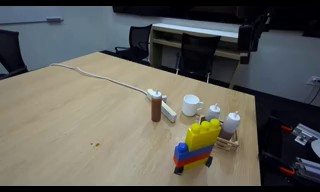
\includegraphics[width=3.8cm]{media/hallucination/lego0.jpg}};
\node[frame] (f2) at (5.9,1.5)  {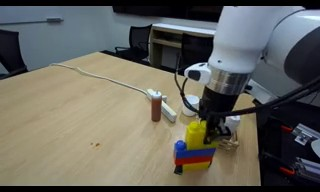
\includegraphics[width=3.8cm]{media/hallucination/lego3.jpg}};
\node[frame] (f3) at (11.8,1.5) {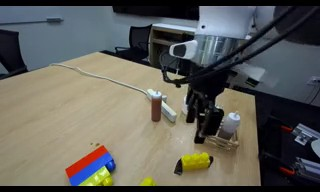
\includegraphics[width=3.8cm]{media/hallucination/lego7.jpg}};
\node[ell] at (2.95,1.5) {$\cdots$};
\node[ell] at (8.85,1.5) {$\cdots$};
% descriptions (real, condensed) -- VLM output, fabrications in red
\node[outtag, text=teal!45!black, anchor=west] at (-2.5,-0.95) {VLM output};
\node[desc] (d1) at (0,-2.0)
  {\textbf{Objects:} yellow, blue and red blocks, and \textcolor{red!75!black}{\bfseries a white and a brown block}. \textbf{Gripper:} not visible. \textbf{Progress:} 1 of 4 stacked, 3 remain.};
\node[desc] (d2) at (5.9,-2.0)
  {\textbf{Objects:} the blocks, stacked. \textbf{Gripper:} holding \textcolor{red!75!black}{\bfseries a white block}. \textbf{Progress:} the block is being placed for stacking.};
\node[desc] (d3) at (11.8,-2.0)
  {\textbf{Objects:} the blocks, scattered again. \textbf{Gripper:} holding \textcolor{red!75!black}{\bfseries a black block}. \textbf{Progress:} the attempt fails; the tower is not taken apart.};
% grade cells -- LLM output
\node[outtag, text=orange!55!black, anchor=west] at (-2.5,-4.35) {LLM output};
\node[grade] (L1) at (0,-5.05)    {{\scriptsize score}\\[1pt]{\large\textbf{1}}};
\node[grade] (L2) at (5.9,-5.05)  {{\scriptsize score}\\[1pt]{\large\textbf{4}}};
\node[grade] (L3) at (11.8,-5.05) {{\scriptsize score}\\[1pt]{\large\textbf{4}}};
% arrows
\draw[->,teal!60!black,thick] (f1) -- (d1);
\draw[->,teal!60!black,thick] (f2) -- (d2);
\draw[->,teal!60!black,thick] (f3) -- (d3);
\draw[->,thick] (d1) -- (L1);
\draw[->,thick] (d2) -- (L2);
\draw[->,thick] (d3) -- (L3);
\draw[->,orange!80!black,thick] (L1) -- node[above=1pt,font=\scriptsize,text=orange!55!black]{$+$ earlier descriptions} (L2);
\draw[->,orange!80!black,thick] (L2) -- node[above=1pt,font=\scriptsize,text=orange!55!black]{$+$ earlier descriptions} (L3);
% stage bands + outer container
\begin{scope}[on background layer]
  \node[fill=teal!5,   rounded corners=4pt, fit=(st1)(tl1)(tl3)(f1)(f3)(d1)(d3), inner sep=8pt] (b1){};
  \node[fill=orange!5, rounded corners=4pt, fit=(st2)(L1)(L3),         inner sep=8pt] (b2){};
  \node[draw=gray!45, line width=0.8pt, rounded corners=6pt, fit=(hdr)(b1)(b2), inner sep=6pt] {};
\end{scope}
\end{tikzpicture}%
}
\caption[A hallucination surviving the pipeline]{A hallucination that survives the two-stage pipeline of Section~\ref{sec:method-real-failures}, shown in the format of Figure~\ref{fig:vlm-llm-pipeline}, on a DROID clip whose task is to unstack a lego tower. The real blocks are yellow, blue and red with a second yellow block on top. The white and brown objects behind them are a cup and a bottle. The VLM's fabrications, in red, report objects that are not there (a white and a brown block), then misread the grasped yellow block as white, and at the end see a black block in an empty gripper. Because each description is stated with confidence, and the reported blocks on the gripper keep changing, the grader is pulled to a full score of four from the fourth frame on, whereas the true progress is closer to two. The arm lifts the top block but then scatters the tower instead of unstacking it. Frames, descriptions, and scores are real outputs.}
\label{fig:vlm-hallucination}
\end{figure}

\chapter{The Loss Study in Detail}
\label{apx:lambda}

The loss study of Section~\ref{sec:results-lora} compares its variants by a single number, the best-checkpoint rank accuracy averaged over the four evaluation splits. This appendix opens that number up. Table~\ref{tab:lora-breakdown} reports every variant of the study at its best checkpoint, with the per-split composition of the demonstration-conditioned aggregate and the demonstration-free aggregate beside it.

\begin{table}[h]
\centering\footnotesize
\caption[The loss study per split]{Every variant of the loss study of Section~\ref{sec:results-lora} at its best checkpoint by the four-split aggregate. The first four columns give the per-split rank accuracy with an in-context demonstration, the last two the aggregates with and without one. The best value per column is in bold.}
\label{tab:lora-breakdown}
\begin{tabular}{@{}lcccccc@{}}
\toprule
 & \multicolumn{4}{c}{with demonstration} & \multicolumn{2}{c}{aggregate} \\
\cmidrule(lr){2-5}\cmidrule(lr){6-7}
Variant & DROID & Robometer & MetaWorld & FailSafe & with & without \\
\midrule
Reweighted $\lambda=0.3$ & 0.572 & \textbf{0.779} & 0.852 & 0.900 & \textbf{0.776} & \textbf{0.757} \\
Reweighted $\lambda=0.5$ & 0.590 & 0.768 & 0.826 & 0.909 & 0.773 & 0.746 \\
CORN $c=0$ & 0.547 & 0.758 & 0.841 & 0.924 & 0.768 & 0.744 \\
CORN $c=0.5$ & 0.544 & 0.713 & 0.811 & 0.932 & 0.750 & 0.732 \\
CORN $c=1.5$ & 0.512 & 0.697 & \textbf{0.882} & 0.918 & 0.752 & 0.747 \\
$\lambda=0.3$ + task dropout & 0.551 & 0.717 & 0.830 & 0.899 & 0.749 & 0.748 \\
$\lambda=0.3$ + KL anchor $0.1$ & \textbf{0.592} & 0.696 & 0.868 & \textbf{0.938} & 0.773 & 0.753 \\
$\lambda=0.3$ + KL anchor $0.3$ & 0.544 & 0.770 & 0.819 & 0.923 & 0.764 & 0.749 \\
\bottomrule
\end{tabular}
\end{table}

Three things stand out in this table. First, the per-split winners scatter, KL $0.1$ takes DROID and FailSafe, the strongest CORN asymmetry takes MetaWorld, yet no variant beats the plain reweighted loss on the aggregate in either mode. Second, DROID is the weakest split for every single variant, roughly $0.51$ to $0.59$ against $0.70$ to $0.94$ everywhere else, the first sign of the pattern the main results confirm at full scale. It also shows what pretraining on ideal demonstrations leaves behind. Robometer never met a real-world failure as a direct training target, so the ability to tell a DROID failure from a success has to be built almost from scratch, and a light adapter on an $18$k sample barely lifts it above chance. It takes the full fine-tunes of Chapter~\ref{sec:results} to raise DROID ranking to $0.734$ (Section~\ref{sec:results-frames}). Third, every best checkpoint falls between steps $500$ and $4{,}000$ of the $7{,}500$-step budget, so the adapters saturate early on this $18$k sample, and the three runs that stopped near step three thousand, CORN $c=0$, $\lambda=0.5$, and the stronger KL anchor, all stopped inside the window where the others peak.

The two aggregate columns carry one more observation. The demonstration lifts every variant of the study, by one to three points, with a single exception: the task-dropout variant, where the two modes land within a tenth of a point of each other. That is the variant that deliberately corrupts the task description on demonstration-carrying samples, so the one configuration built to disturb the language channel of in-context learning is also the one whose demonstration gain disappears. The demonstrations were already paying off at LoRA scale, before any full fine-tune, and the dropout that was meant to strengthen them erased their advantage instead.

\section{Choosing the asymmetry strength}

The main text reports the reweighted loss at a single asymmetry strength, $\lambda = 0.3$, selected against a milder $\lambda = 0.5$ that corrects under-predictions at half strength instead of a third. Table~\ref{tab:lambda-sweep} gives that comparison in full, both variants at their best checkpoint, with and without an in-context demonstration.

\begin{table}[h]
\centering\footnotesize
\caption[Choosing the asymmetry strength]{Rank accuracy of the reweighted loss at two asymmetry strengths, each at its best checkpoint by the four-split aggregate, evaluated with and without an in-context demonstration. The stronger $\lambda = 0.3$ takes the aggregate in both modes, with the differences concentrated on MetaWorld.}
\label{tab:lambda-sweep}
\begin{tabular}{@{}lcccc@{}}
\toprule
 & \multicolumn{2}{c}{with demonstration} & \multicolumn{2}{c}{without} \\
\cmidrule(lr){2-3}\cmidrule(lr){4-5}
Split & $\lambda=0.3$ & $\lambda=0.5$ & $\lambda=0.3$ & $\lambda=0.5$ \\
\midrule
DROID & 0.572 & \textbf{0.590} & 0.517 & \textbf{0.534} \\
Robometer & \textbf{0.779} & 0.768 & 0.794 & \textbf{0.808} \\
MetaWorld & \textbf{0.852} & 0.826 & \textbf{0.791} & 0.717 \\
FailSafe & 0.900 & \textbf{0.909} & \textbf{0.928} & 0.926 \\
\midrule
Aggregate & \textbf{0.776} & 0.773 & \textbf{0.757} & 0.746 \\
\bottomrule
\end{tabular}
\end{table}

The two strengths are close, which is itself the useful finding. Doubling down on the asymmetry costs the reweighted loss essentially nothing in ranking quality, the aggregate favors $\lambda = 0.3$ in both modes, and the one split with a clear gap, MetaWorld without a demonstration, favors it by seven points. This stands in direct contrast to the ordinal family of Table~\ref{tab:lora-breakdown}, whose ranking degrades as its asymmetry $c$ grows, and it is why we keep the stronger setting: at equal or better ranking quality, $\lambda = 0.3$ buys more of the conservatism the loss exists to provide.

\chapter{Length Bias in Video-Based Reward Models}
\label{apx:length-bias}

Section~\ref{sec:method-arch} samples a fixed number of frames from every trajectory instead of passing the raw video to the model. This is what Robometer follows as well, and according to our preliminary tests this is in the right direction. This appendix sheds some light on these decisions. Before adopting Robometer, which came out in March 2026, we were building on RoboReward \citep{roboreward}, which scores a whole video at once instead of feeding separate frames. There, we found that its score was biased by the video length. A reward that reads length as a stand-in for failure is easy for a policy to fool, which is what pushed us toward a fixed frame budget. The study below is small and predates our main experiments based on Robometer, but we consider this study relevant, as it reveals the significance of using frames as input to vision-language reward models.

The confound begins in the training data. RoboReward manufactures most of its negatives by truncating successful episodes, cutting a completed attempt short so that it no longer reaches the goal. Across the 45{,}072 videos of its released dataset, 11{,}116 of the lower-reward examples are these temporal clips, the same task with the video cut off partway, against only 3{,}228 counterfactual relabels. The average full episode runs about 31 seconds and the average clip about 9.5. Shorter therefore correlates with failure by construction. The effect is amplified at inference, because the video-loading path samples frames at a fixed rate of two per second by default, so a shorter clip is also seen through fewer frames. A model trained this way can pick up a shortcut, that few frames means failure, which has nothing to do with the task itself.

To probe RoboReward-8B for this shortcut, we evaluated the model as a binary classifier, asking a simple yes-or-no question for each clip: did the attempt succeed? We framed the evaluation this way for two reasons. First, the clips in our dataset carry a binary ground truth, they are either genuine successes or truncated failures, so metrics like recall and the confusion matrix require a binary prediction to be meaningful. Second, this mirrors how such a reward is actually used in practice; a policy ultimately acts on a hard success decision dictated by a threshold, not a soft continuous score. 

While we inherited the one-to-five scoring concept from RoboReward, we adapted it to fit our approach. This introduced two key differences:
\begin{itemize}
    \item \textbf{Granularity:} RoboReward assigns a single holistic score to the entire trajectory, where 5 is a clean success and 1 is no progress at all. In contrast, our model outputs a dense, per-frame progress signal. 
    \item \textbf{Specificity:} RoboReward relies on more abstract definitions for its intermediate scores (2, 3, and 4). We explicitly defined these intermediate states later in our own implementation. 
\end{itemize}

To convert RoboReward's trajectory-level score into a binary verdict for our confusion matrices, we imposed a threshold of 3.5. Any prediction of 3.5 or higher is counted as a success, while anything below is a failure. We chose this deliberately lenient cutoff for this specific analysis so that a ``mostly successful'' score of 4 still passes as a success. Later, in our configuration, we enforced a stricter approach by accepting only a 5 as a success. It should be noted, however, that the length effect we report holds true regardless of where this initial threshold is drawn.

\begin{figure}[h]
\centering
\begin{minipage}[b]{0.49\textwidth}
  \centering
  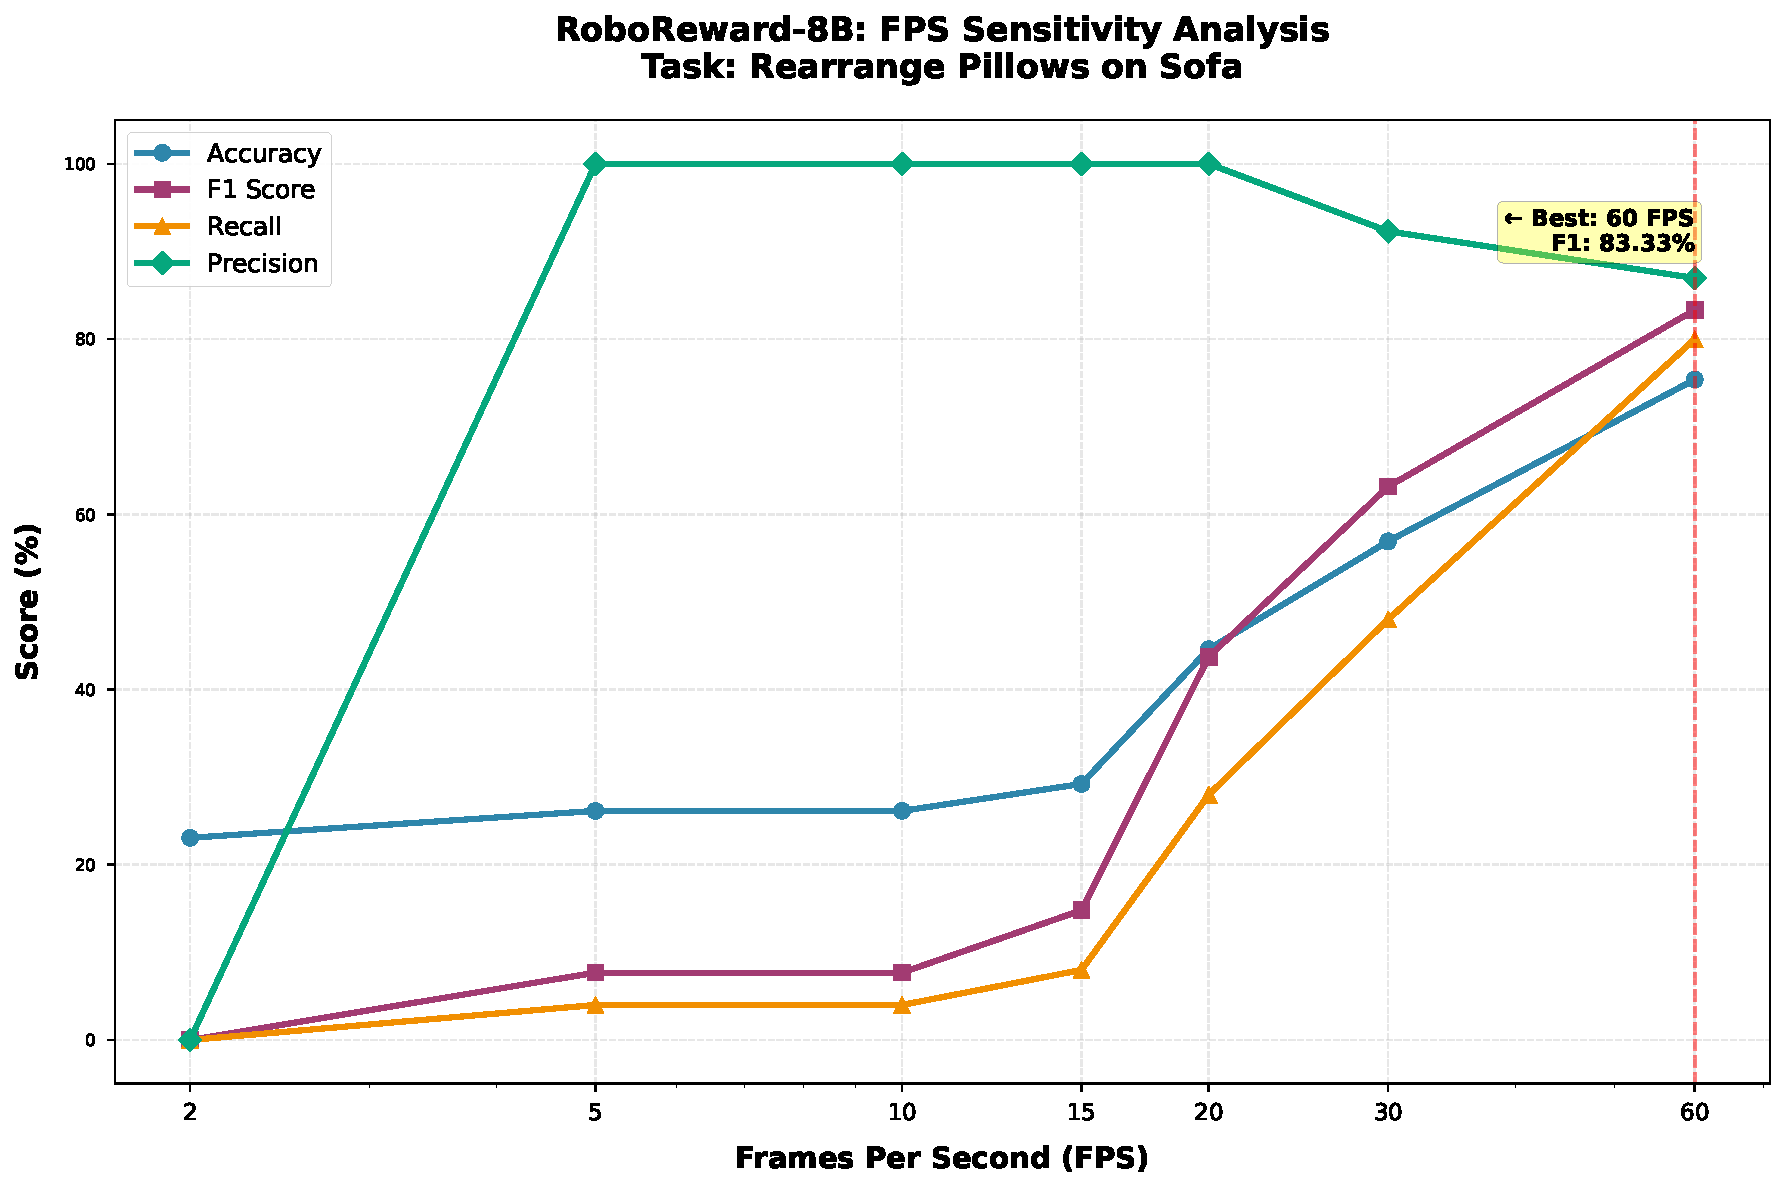
\includegraphics[width=\textwidth]{media/length-bias/fps_sweep.pdf}\\
  {\footnotesize (a) Frame-sampling sweep}
\end{minipage}\hfill
\begin{minipage}[b]{0.49\textwidth}
  \centering
  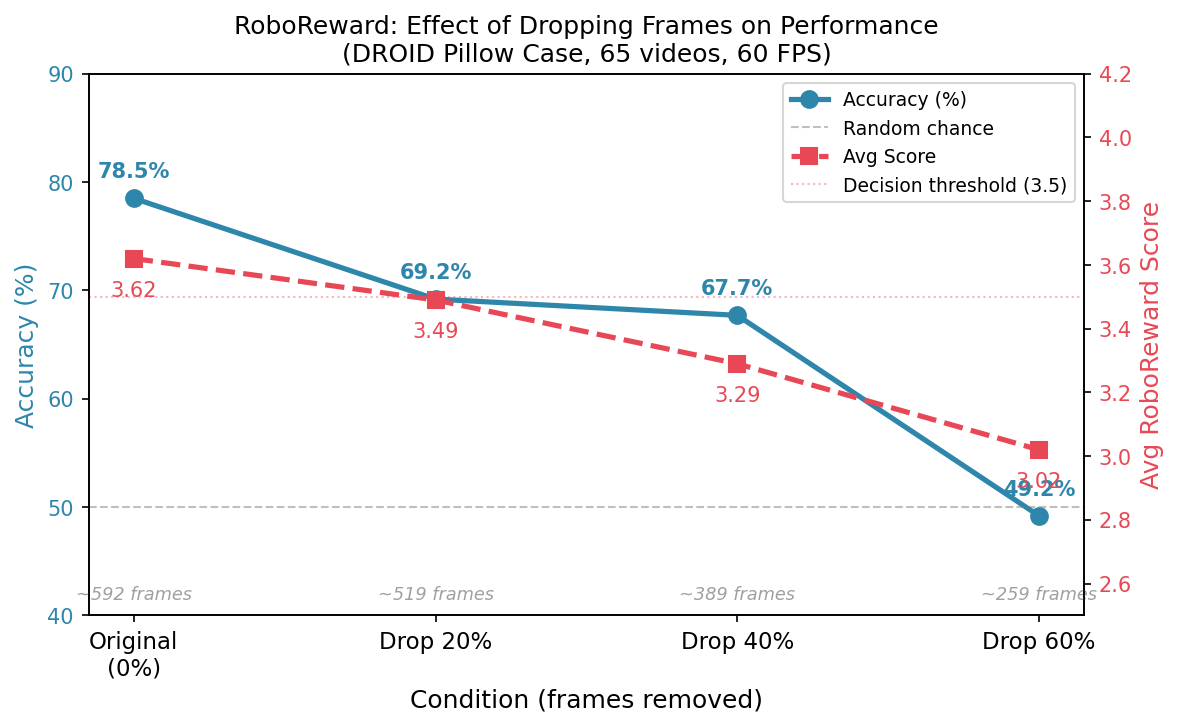
\includegraphics[width=\textwidth]{media/length-bias/frame_drop.png}\\
  {\footnotesize (b) Frame drop at fixed rate}
\end{minipage}
\caption[RoboReward scores video length, not content]{RoboReward-8B scores video length as much as content, on 65 DROID pillow-rearranging clips (50 success, 15 failure). \emph{(a)} As the frame-sampling rate falls, recall collapses toward zero, so successful attempts read as failures purely because they are seen through fewer frames. \emph{(b)} Holding the rate fixed at 60 frames per second and instead dropping a uniform fraction of the frames, with the visible content unchanged, accuracy falls from 78.5 to 49.2 percent and the mean score crosses the 3.5 success cutoff (scores at or above 3.5 count as a predicted success), flipping 25 of the 65 predictions. This is the length shortcut that motivates giving RoboRef a fixed frame budget in Section~\ref{sec:method-arch}.}
\label{fig:length-bias}
\end{figure}

First we swept the frame-sampling rate. On a set of 65 DROID clips of a pillow-rearranging task, 50 successes and 15 failures recorded at 60 frames per second, we varied the sampling rate from the library default up to the native rate and read off the verdict at each rate. At the default of two frames per second the model called every one of the 50 successful clips a failure, a recall of zero, and only as the frame count climbed did success become recognizable, reaching a recall of 80 percent near the native rate. Figure~\ref{fig:length-bias}~(a) shows the sweep. We saw the same collapse on data drawn from RoboReward's own training distribution, where recall moved from 5 percent at two frames per second to 80 percent at the native ten. The rate that worked best tracked each dataset's native frame count and not any fixed value, which is what a frame-count artifact would predict and genuine task understanding would not.

The sweep changes two things at once, the number of frames and the timestamps the model reads, so we ran a cleaner test that varies only the frame count. Holding the sampling rate fixed at 60 frames per second, we extracted every frame and then dropped a uniform fraction of them before scoring, leaving the visible content otherwise untouched. Figure~\ref{fig:length-bias}~(b) shows what happens. Removing frames drives accuracy down from 78.5 percent on the full clips to 49.2 percent, no better than chance. The mean score falls with it, from 3.62 on the full clips, comfortably on the success side of the 3.5 cutoff, down to 3.02, now on the failure side, so the average clip flips its verdict from success to failure. A quarter of the individual predictions, 25 of the 65, flip the same way, with no change at all to what the video shows. The same attempt, seen through fewer frames, reads as a failure.

We present these results with two important notes. The samples are small and imbalanced, 65 clips with only 15 failures, so these are pilot-scale numbers on a single prior model, not a controlled benchmark. Also, the study probes RoboReward, not our own model, so it only motivates a design decision. That decision is to hand the reward model a fixed number of frames per trajectory, eight in Robometer and sixteen in ours, evenly spaced regardless of how long the attempt lasts. A shorter or longer episode is then always seen through the same window, so length can no longer stand in for progress, and the model is forced to judge the attempt on what the frames show.

\chapter{The Conditional-Mean Readout of the Progress Head}
\label{apx:condmean}

The progress columns of the out-of-distribution evaluation, Table~\ref{tab:offline-ood}, are decoded differently from every other number in this thesis, and this appendix explains why, shows the model outputs behind the choice, and answers the objection the choice raises. Robometer's progress head is discrete. It places a probability on each of ten progress bins, and the released pipeline turns this into a scalar by taking the expectation, the probability-weighted mean of the bin centers. The in-distribution results of Tables~\ref{tab:offline-id-rank} and~\ref{tab:offline-id-succ} use that same readout. On the held-out-robot set it stops being usable for the fine-tuned models, because their bin distributions turn bimodal, with a large share of the mass parked on the lowest bin and most of the remainder concentrated near the top. The expectation of such a mixture lands between the two modes, at a value the model itself considers unlikely, and more importantly it multiplies the informative part of the prediction by one minus the lowest-bin mass. Whether the ordering of clips survives that multiplication depends entirely on how that mass behaves across clips. Figure~\ref{fig:bimodal-bins} shows the shape directly for RoboRef-Asym, averaged over thirty successful and thirty failed clips of a manipulation task from its training corpus.

\begin{figure*}[h]
  \centering
  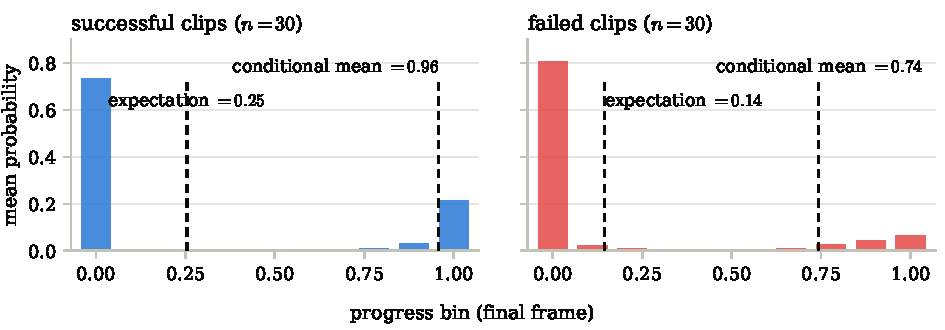
\includegraphics[width=0.93\textwidth]{media/results/bimodal_bins_readouts.pdf}
  \caption[Bimodal progress-bin distributions]{The average final-frame bin distribution of the asymmetric fine-tune on clips of a training task, split by outcome. Both distributions are bimodal, with a large share of the probability on the lowest bin and most of the rest near the top. The expectation lands between the two modes, at a value the model itself gives almost no probability, and reads a genuine success at $0.25$. The conditional mean ignores the lowest bin and reads the same clips at $0.96$ and $0.74$, the right order with a wider gap between the outcomes.}
  \label{fig:bimodal-bins}
\end{figure*}

We therefore decode the progress head with the conditional mean, the same expectation taken after the lowest bin is dropped and the remaining nine renormalized. It answers a narrower question, namely how far the clip has progressed given that the model sees progress at all. Table~\ref{tab:offline-ood} applies it to every model. For the baseline this changes nothing, its distributions are unimodal with almost no mass on the lowest bin, and its two progress columns move by less than a point under the new decode, so the transform cannot be favoring our models by construction. For the fine-tuned models the effect is large. The asymmetric model's Kendall's $\tau$ on this set is $0.16$ under the plain expectation and the $0.58$ reported in the table under the conditional mean.

The natural objection is that the in-distribution results of Tables~\ref{tab:offline-id-rank} and~\ref{tab:offline-id-succ}, which keep the plain expectation, should suffer from the same problem, since the same failure-heavy training produced the same bimodal heads there. They do not, and the reason is that rank metrics are indifferent to any distortion that preserves order. In distribution the lowest-bin mass is systematic, failures carry visibly more of it than successes, so scaling every score by one minus that mass compresses the numbers but keeps them in the right order, and rank accuracy and $\tau$ cannot tell the difference. On held-out robots the same mass stops tracking the task and starts tracking the unfamiliar embodiment. Measured on the held-out-robot set for the asymmetric fine-tune, successful clips carry a mean lowest-bin mass of $0.70$ and failed ones $0.71$, a gap of $0.01$ between the classes against a within-class spread of $0.07$. A factor seven times as noisy as it is informative scrambles any ordering it multiplies, which is what the plain expectation shows, and dividing it out is what restores it. Figure~\ref{fig:hedge-mass} shows the contrast directly. The same effect sits behind part~(a) of Figure~\ref{fig:offline-qual}, where the completed out-of-distribution success is read at $0.21$ by the plain expectation.

\begin{figure*}[h]
  \centering
  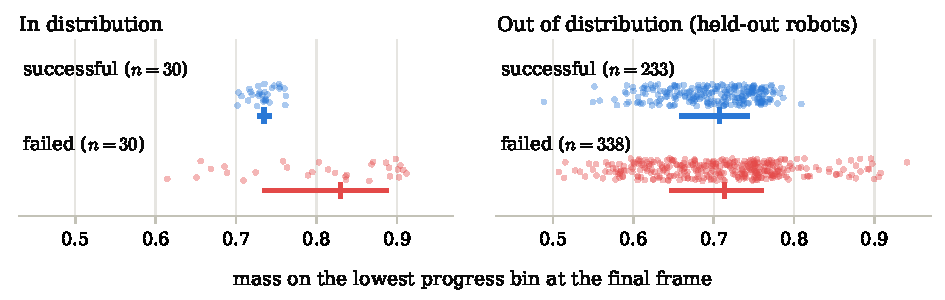
\includegraphics[width=0.93\textwidth]{media/results/hedge_mass_id_vs_ood.pdf}
  \caption[Why the conditional mean is needed only out of distribution]{Why the conditional mean is needed out of distribution and not in distribution, shown on the asymmetric fine-tune. Each dot is one clip. Its position shows how much probability the model puts on the lowest progress bin at the final frame, in other words how strongly the model votes that the clip shows no progress. The plain expectation scales a clip's score by one minus this value, so clips further to the right end up with smaller scores. The short vertical line under each group marks the median clip and the horizontal bar spans the middle half of the group. In distribution (left, clips of a training task) the vote is accurate. Failed clips sit clearly to the right of successful ones, their scores shrink more, and the final scores still rank successes above failures. On the held-out robots of Table~\ref{tab:offline-ood} (right) successful and failed clips receive almost the same vote on average while individual clips of either kind vary widely, so the shrinking is essentially random and it shuffles the final scores. The conditional mean removes this factor, which is what restores the ranking.}
  \label{fig:hedge-mass}
\end{figure*}

\chapter{Reward Received During MetaWorld Training}
\label{apx:mw-reward}

This appendix expands the reward-hacking analysis that Section~\ref{sec:results-rl-mw} summarizes. Figure~\ref{fig:mw-reward} plots the reward the policy actually received during training, the mean per-step value the reward model returned, for our three RoboRef fine-tunes and the released Robometer-4B, which all read the same success head and so pay on one comparable scale. This is the model's own reward and not the true task reward, and the success rates of Figure~\ref{fig:mw-rl} remain the ground truth throughout.

On Coffee-Push the released Robometer-4B pays the policy the most reward of any model, by a wide margin, roughly $0.04$ per step against the asymmetric fine-tunes' $0.01$ to $0.02$, while training a policy whose true success rate is zero. A reward that grows while success does not is the signature of reward hacking, since the policy has found the false positives the model's offline overconfidence promised (Figure~\ref{fig:offline-qual}) and learned to manufacture them, collecting a reward it never earned. The asymmetric fine-tunes tell the opposite story, paying a smaller reward that climbs together with true success, the shape of a signal being earned, not gamed, while RoboRef-Std fires rarely and pays almost nothing, moving the policy little. The difference between Robometer-4B and RoboRef-Std is our failure data, which taught the latter to reject the near-misses MetaWorld policies actually produce, so the blatant false positives the released model farms are gone. What remains is the opposite problem, a reward so hesitant that it underpays genuine progress, and this starves the policy where the released model misleads it. The dense-reward baselines sit on scales that cannot be read against these. In short, the reward a policy collects is a poor proxy for the policy it becomes, and holding the two apart is precisely the job of the conservative loss.


\begin{figure*}[h]
\centering
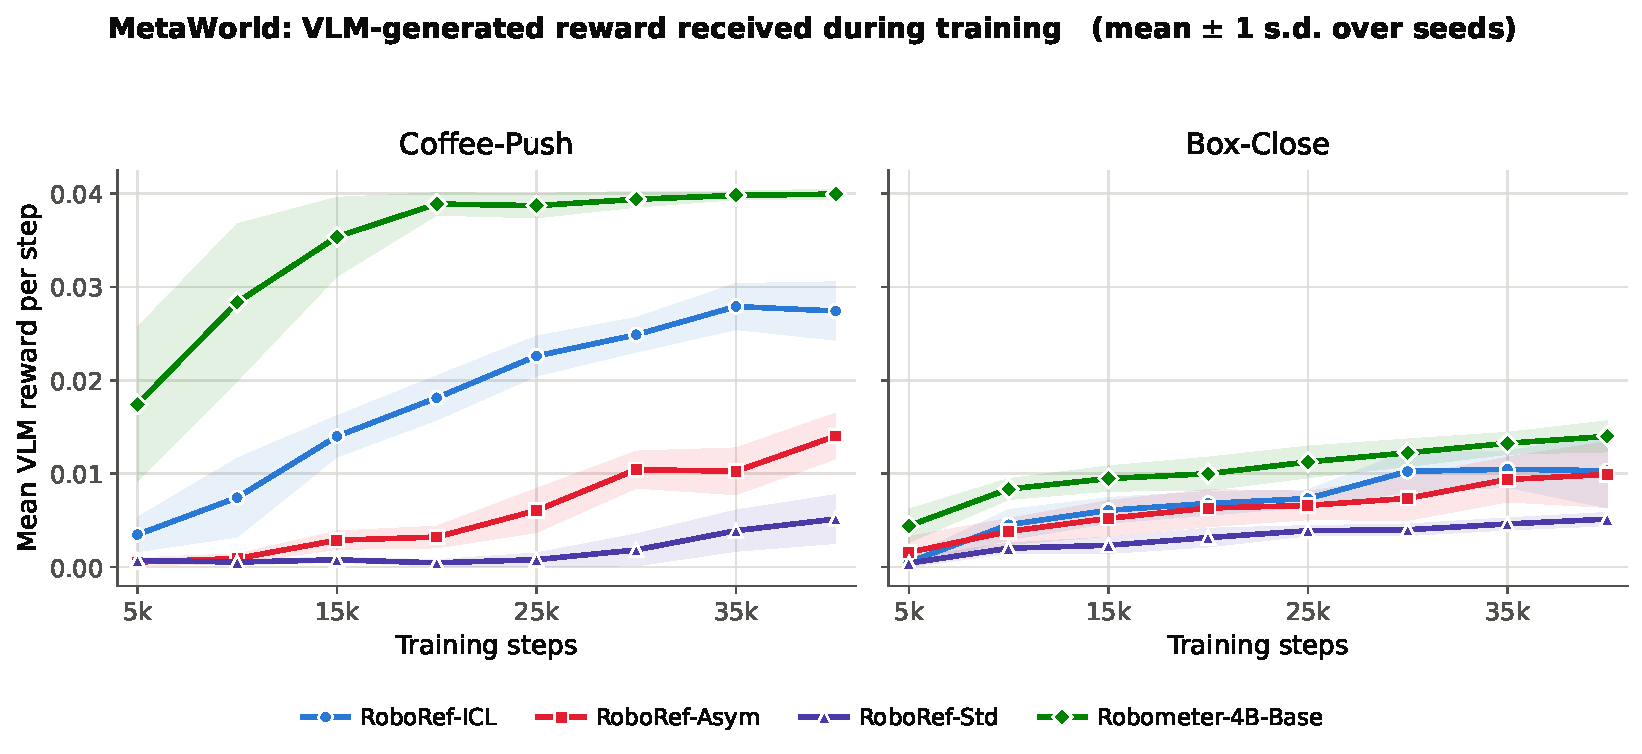
\includegraphics[width=\textwidth]{media/results/metaworld_reward.pdf}
\caption[VLM reward received during MetaWorld training]{The vision-language reward the policy received during training, mean per-step value returned by the reward model, for our three RoboRef fine-tunes and the released Robometer-4B, which share one success-probability scale and are therefore comparable. This is the model's own reward, not the true task reward of Figure~\ref{fig:mw-rl}. On Coffee-Push the released Robometer-4B pays the most reward of any model yet its policy never succeeds, the mark of farmed false positives; the asymmetric fine-tunes pay a smaller reward that rises with genuine success.}
\label{fig:mw-reward}
\end{figure*}

Lastly, we underline that the result is not an artifact of how the comparison is implemented. Every reward in the figure is calibrated by the same procedure and held to the same minimum length, and every baseline still fails, so the advantage can only sit in the reward itself, its refusal to pay out on the near-misses a policy will otherwise learn to manufacture.


\chapter{Examples of Generated Failure Data}
\label{apx:gallery}

This appendix shows a sample of the failure trajectories we generate in simulation, the data described in Section~\ref{sec:method-sim-failures}. Each example is a short filmstrip of a single failed attempt, and the number above each frame is its ground-truth progress score, read directly from the simulator state. The scores run from $1$ (no progress) to $5$ (success), so a failed attempt never exceeds $4$.

We group the examples by the score the attempt reaches, so each block illustrates what a given level of partial progress looks like across different tasks and different ways of failing. The failure modes the generator can use depend on how far the attempt gets. Early failures look like random flailing or motion in the wrong direction, mid-progress failures hold an object and then freeze or push it the wrong way, and near-complete failures grasp or place the object and then drop or misplace it at the last moment. The scores follow the behavior, including downward when an object is dropped, which is the property a monotone $t/T$ label cannot capture.

\section{Tasks and failure modes}

Both simulated benchmarks generate failures by injecting a fault into a scripted policy, as described in Section~\ref{sec:method-sim-failures}. The kind of failure that comes out depends on the task family and the target score. Table~\ref{tab:sim-modes} lists the nine noise modes we use in MetaWorld \citep{yu_meta-world_2019} and where each applies, and Table~\ref{tab:sim-tasks} lists the tasks by family.

\begin{table}[t]
\centering\footnotesize
\caption[MetaWorld noise modes]{The nine MetaWorld noise modes and the family and score at which each is applied. Scores~1 and~2 use the same modes across every family; the higher scores are family-specific.}
\label{tab:sim-modes}
\begin{tabular}{@{}p{2.4cm}p{5.9cm}p{4.7cm}@{}}
\toprule
Mode & Behavior & Applied at \\
\midrule
random & fully random actions & score 1 (all families) \\
wrong-direction & a strong bias away from the goal & score 1 (all); score 3 (grasp-and-move) \\
freeze & the arm holds its position & scores 2--4 (all families) \\
drop & the gripper is forced open mid-transport & score 3 (grasp-and-move) \\
late-drop & the gripper is forced open near the goal & score 4 (grasp-and-move) \\
misplace & the expert action with a small offset near the goal & score 4 (grasp-and-move, push-and-sweep) \\
lift-away & the arm lifts off and loses contact & score 3 (push-and-sweep) \\
push-sideways & the arm pushes perpendicular to the goal & scores 3--4 (push-and-sweep) \\
partial-actuation & the expert drives the mechanism most of the way, then stalls & score 4 (mechanism, press) \\
\bottomrule
\end{tabular}
\end{table}

\begin{table}[t]
\centering\footnotesize
\caption[MetaWorld tasks by family]{The 46 MetaWorld tasks by family, with the scores each family covers. Mechanism and press tasks skip score~3, whose single actuation has no meaningful partial state.}
\label{tab:sim-tasks}
\begin{tabular}{@{}p{2.3cm}cp{9.0cm}@{}}
\toprule
Family & Scores & Tasks \\
\midrule
Grasp-and-move & 1--4 & assembly, basketball, bin-picking, box-close, coffee-pull, hammer, hand-insert, pick-out-of-hole, pick-place, pick-place-wall, shelf-place, stick-pull, stick-push \\
\addlinespace
Push-and-sweep & 1--4 & coffee-push, plate-slide, plate-slide-side, plate-slide-back, plate-slide-back-side, push, push-wall, push-back, soccer, sweep, sweep-into \\
\addlinespace
Mechanism & 1, 2, 4 & dial-turn, disassemble, door-open, door-close, door-lock, door-unlock, drawer-open, drawer-close, faucet-open, faucet-close, handle-press, handle-press-side, handle-pull, handle-pull-side, lever-pull, window-open, window-close \\
\addlinespace
Press & 1, 2, 4 & button-press, button-press-wall, button-press-topdown, button-press-topdown-wall, coffee-button \\
\bottomrule
\end{tabular}
\end{table}

FailSafe \citep{lin_failsafe_2025} adds three ManiSkill \citep{tao_maniskill3_2024} tasks, \texttt{FailPickCube} (lift a cube to a goal), \texttt{FailPushCube} (push a cube to a goal), and \texttt{FailStackCube} (stack a red cube on a green one), scored on the same one-to-five scale. Each task is driven by a scripted multi-stage planner, reach, grasp, lift, align, place, and a fault is injected at a chosen stage. The stage sets the score, so a fault early in the plan yields a low score and one at the last stage a near-complete score-4 failure. The injected fault fits the stage, a grasp that is then released or frozen, a push that stalls or veers off, or a cube carried and dropped just short of the target. Stacking is the only FailSafe task with a meaningful score~3, a cube grasped and held or carried but not yet placed.

\section{Score 1: no meaningful progress}
{\centering
\setlength{\tabcolsep}{1pt}\renewcommand{\arraystretch}{0.5}
\begin{tabular}{@{}cccccccc@{}}
{\scriptsize 1} & {\scriptsize 1} & {\scriptsize 1} & {\scriptsize 1} & {\scriptsize 1} & {\scriptsize 1} & {\scriptsize 1} & {\scriptsize 1} \\

\includegraphics[width=0.118\textwidth]{media/appendix/s1_window/f0.jpg} &

\includegraphics[width=0.118\textwidth]{media/appendix/s1_window/f1.jpg} &

\includegraphics[width=0.118\textwidth]{media/appendix/s1_window/f2.jpg} &

\includegraphics[width=0.118\textwidth]{media/appendix/s1_window/f3.jpg} &

\includegraphics[width=0.118\textwidth]{media/appendix/s1_window/f4.jpg} &

\includegraphics[width=0.118\textwidth]{media/appendix/s1_window/f5.jpg} &

\includegraphics[width=0.118\textwidth]{media/appendix/s1_window/f6.jpg} &

\includegraphics[width=0.118\textwidth]{media/appendix/s1_window/f7.jpg} \\
\end{tabular}\\[2pt]
{\footnotesize Window-close, random actions.}\par}
\vspace{8pt}
{\centering
\setlength{\tabcolsep}{1pt}\renewcommand{\arraystretch}{0.5}
\begin{tabular}{@{}cccccccc@{}}
{\scriptsize 1} & {\scriptsize 1} & {\scriptsize 1} & {\scriptsize 1} & {\scriptsize 1} & {\scriptsize 1} & {\scriptsize 1} & {\scriptsize 1} \\

\includegraphics[width=0.118\textwidth]{media/appendix/s1_door/f0.jpg} &

\includegraphics[width=0.118\textwidth]{media/appendix/s1_door/f1.jpg} &

\includegraphics[width=0.118\textwidth]{media/appendix/s1_door/f2.jpg} &

\includegraphics[width=0.118\textwidth]{media/appendix/s1_door/f3.jpg} &

\includegraphics[width=0.118\textwidth]{media/appendix/s1_door/f4.jpg} &

\includegraphics[width=0.118\textwidth]{media/appendix/s1_door/f5.jpg} &

\includegraphics[width=0.118\textwidth]{media/appendix/s1_door/f6.jpg} &

\includegraphics[width=0.118\textwidth]{media/appendix/s1_door/f7.jpg} \\
\end{tabular}\\[2pt]
{\footnotesize Door-open, wanders off, never reaches the door.}\par}
\vspace{8pt}
{\centering
\setlength{\tabcolsep}{1pt}\renewcommand{\arraystretch}{0.5}
\begin{tabular}{@{}cccccccc@{}}
{\scriptsize 1} & {\scriptsize 1} & {\scriptsize 1} & {\scriptsize 1} & {\scriptsize 1} & {\scriptsize 1} & {\scriptsize 1} & {\scriptsize 1} \\

\includegraphics[width=0.118\textwidth]{media/appendix/s1_push/f0.jpg} &

\includegraphics[width=0.118\textwidth]{media/appendix/s1_push/f1.jpg} &

\includegraphics[width=0.118\textwidth]{media/appendix/s1_push/f2.jpg} &

\includegraphics[width=0.118\textwidth]{media/appendix/s1_push/f3.jpg} &

\includegraphics[width=0.118\textwidth]{media/appendix/s1_push/f4.jpg} &

\includegraphics[width=0.118\textwidth]{media/appendix/s1_push/f5.jpg} &

\includegraphics[width=0.118\textwidth]{media/appendix/s1_push/f6.jpg} &

\includegraphics[width=0.118\textwidth]{media/appendix/s1_push/f7.jpg} \\
\end{tabular}\\[2pt]
{\footnotesize Push, moves the wrong way.}\par}
\vspace{8pt}
{\centering
\setlength{\tabcolsep}{1pt}\renewcommand{\arraystretch}{0.5}
\begin{tabular}{@{}cccccccc@{}}
{\scriptsize 1} & {\scriptsize 1} & {\scriptsize 1} & {\scriptsize 1} & {\scriptsize 1} & {\scriptsize 1} & {\scriptsize 1} & {\scriptsize 1} \\

\includegraphics[width=0.118\textwidth]{media/appendix/s1_hammer/f0.jpg} &

\includegraphics[width=0.118\textwidth]{media/appendix/s1_hammer/f1.jpg} &

\includegraphics[width=0.118\textwidth]{media/appendix/s1_hammer/f2.jpg} &

\includegraphics[width=0.118\textwidth]{media/appendix/s1_hammer/f3.jpg} &

\includegraphics[width=0.118\textwidth]{media/appendix/s1_hammer/f4.jpg} &

\includegraphics[width=0.118\textwidth]{media/appendix/s1_hammer/f5.jpg} &

\includegraphics[width=0.118\textwidth]{media/appendix/s1_hammer/f6.jpg} &

\includegraphics[width=0.118\textwidth]{media/appendix/s1_hammer/f7.jpg} \\
\end{tabular}\\[2pt]
{\footnotesize Hammer, random actions.}\par}
\vspace{8pt}

\bigskip

\section{Score 2: object approached but not engaged}
{\centering
\setlength{\tabcolsep}{1pt}\renewcommand{\arraystretch}{0.5}
\begin{tabular}{@{}cccccccc@{}}
{\scriptsize 2} & {\scriptsize 2} & {\scriptsize 2} & {\scriptsize 2} & {\scriptsize 2} & {\scriptsize 2} & {\scriptsize 2} & {\scriptsize 2} \\

\includegraphics[width=0.118\textwidth]{media/appendix/s2_faucet/f0.jpg} &

\includegraphics[width=0.118\textwidth]{media/appendix/s2_faucet/f1.jpg} &

\includegraphics[width=0.118\textwidth]{media/appendix/s2_faucet/f2.jpg} &

\includegraphics[width=0.118\textwidth]{media/appendix/s2_faucet/f3.jpg} &

\includegraphics[width=0.118\textwidth]{media/appendix/s2_faucet/f4.jpg} &

\includegraphics[width=0.118\textwidth]{media/appendix/s2_faucet/f5.jpg} &

\includegraphics[width=0.118\textwidth]{media/appendix/s2_faucet/f6.jpg} &

\includegraphics[width=0.118\textwidth]{media/appendix/s2_faucet/f7.jpg} \\
\end{tabular}\\[2pt]
{\footnotesize Faucet-open, reaches then freezes.}\par}
\vspace{8pt}
{\centering
\setlength{\tabcolsep}{1pt}\renewcommand{\arraystretch}{0.5}
\begin{tabular}{@{}cccccccc@{}}
{\scriptsize 1} & {\scriptsize 1} & {\scriptsize 1} & {\scriptsize 1} & {\scriptsize 2} & {\scriptsize 2} & {\scriptsize 2} & {\scriptsize 2} \\

\includegraphics[width=0.118\textwidth]{media/appendix/s2_door/f0.jpg} &

\includegraphics[width=0.118\textwidth]{media/appendix/s2_door/f1.jpg} &

\includegraphics[width=0.118\textwidth]{media/appendix/s2_door/f2.jpg} &

\includegraphics[width=0.118\textwidth]{media/appendix/s2_door/f3.jpg} &

\includegraphics[width=0.118\textwidth]{media/appendix/s2_door/f4.jpg} &

\includegraphics[width=0.118\textwidth]{media/appendix/s2_door/f5.jpg} &

\includegraphics[width=0.118\textwidth]{media/appendix/s2_door/f6.jpg} &

\includegraphics[width=0.118\textwidth]{media/appendix/s2_door/f7.jpg} \\
\end{tabular}\\[2pt]
{\footnotesize Door-open, reaches then freezes.}\par}
\vspace{8pt}
{\centering
\setlength{\tabcolsep}{1pt}\renewcommand{\arraystretch}{0.5}
\begin{tabular}{@{}cccccccc@{}}
{\scriptsize 1} & {\scriptsize 1} & {\scriptsize 1} & {\scriptsize 2} & {\scriptsize 2} & {\scriptsize 2} & {\scriptsize 2} & {\scriptsize 2} \\

\includegraphics[width=0.118\textwidth]{media/appendix/s2_sweep/f0.jpg} &

\includegraphics[width=0.118\textwidth]{media/appendix/s2_sweep/f1.jpg} &

\includegraphics[width=0.118\textwidth]{media/appendix/s2_sweep/f2.jpg} &

\includegraphics[width=0.118\textwidth]{media/appendix/s2_sweep/f3.jpg} &

\includegraphics[width=0.118\textwidth]{media/appendix/s2_sweep/f4.jpg} &

\includegraphics[width=0.118\textwidth]{media/appendix/s2_sweep/f5.jpg} &

\includegraphics[width=0.118\textwidth]{media/appendix/s2_sweep/f6.jpg} &

\includegraphics[width=0.118\textwidth]{media/appendix/s2_sweep/f7.jpg} \\
\end{tabular}\\[2pt]
{\footnotesize Sweep-into, touches then freezes.}\par}
\vspace{8pt}
{\centering
\setlength{\tabcolsep}{1pt}\renewcommand{\arraystretch}{0.5}
\begin{tabular}{@{}cccccccc@{}}
{\scriptsize 1} & {\scriptsize 1} & {\scriptsize 1} & {\scriptsize 1} & {\scriptsize 2} & {\scriptsize 2} & {\scriptsize 2} & {\scriptsize 2} \\

\includegraphics[width=0.118\textwidth]{media/appendix/s2_drawer/f0.jpg} &

\includegraphics[width=0.118\textwidth]{media/appendix/s2_drawer/f1.jpg} &

\includegraphics[width=0.118\textwidth]{media/appendix/s2_drawer/f2.jpg} &

\includegraphics[width=0.118\textwidth]{media/appendix/s2_drawer/f3.jpg} &

\includegraphics[width=0.118\textwidth]{media/appendix/s2_drawer/f4.jpg} &

\includegraphics[width=0.118\textwidth]{media/appendix/s2_drawer/f5.jpg} &

\includegraphics[width=0.118\textwidth]{media/appendix/s2_drawer/f6.jpg} &

\includegraphics[width=0.118\textwidth]{media/appendix/s2_drawer/f7.jpg} \\
\end{tabular}\\[2pt]
{\footnotesize Drawer-open, reaches the handle but never grips it.}\par}
\vspace{8pt}

\bigskip

\section{Score 3: object engaged, partial progress}
{\centering
\setlength{\tabcolsep}{1pt}\renewcommand{\arraystretch}{0.5}
\begin{tabular}{@{}cccccccc@{}}
{\scriptsize 1} & {\scriptsize 2} & {\scriptsize 2} & {\scriptsize 2} & {\scriptsize 3} & {\scriptsize 3} & {\scriptsize 3} & {\scriptsize 3} \\

\includegraphics[width=0.118\textwidth]{media/appendix/s3_bball/f0.jpg} &

\includegraphics[width=0.118\textwidth]{media/appendix/s3_bball/f1.jpg} &

\includegraphics[width=0.118\textwidth]{media/appendix/s3_bball/f2.jpg} &

\includegraphics[width=0.118\textwidth]{media/appendix/s3_bball/f3.jpg} &

\includegraphics[width=0.118\textwidth]{media/appendix/s3_bball/f4.jpg} &

\includegraphics[width=0.118\textwidth]{media/appendix/s3_bball/f5.jpg} &

\includegraphics[width=0.118\textwidth]{media/appendix/s3_bball/f6.jpg} &

\includegraphics[width=0.118\textwidth]{media/appendix/s3_bball/f7.jpg} \\
\end{tabular}\\[2pt]
{\footnotesize Basketball, grasps the ball but never lifts it to the hoop.}\par}
\vspace{8pt}
{\centering
\setlength{\tabcolsep}{1pt}\renewcommand{\arraystretch}{0.5}
\begin{tabular}{@{}cccccccc@{}}
{\scriptsize 1} & {\scriptsize 1} & {\scriptsize 1} & {\scriptsize 2} & {\scriptsize 3} & {\scriptsize 3} & {\scriptsize 3} & {\scriptsize 3} \\

\includegraphics[width=0.118\textwidth]{media/appendix/s3_pickpl/f0.jpg} &

\includegraphics[width=0.118\textwidth]{media/appendix/s3_pickpl/f1.jpg} &

\includegraphics[width=0.118\textwidth]{media/appendix/s3_pickpl/f2.jpg} &

\includegraphics[width=0.118\textwidth]{media/appendix/s3_pickpl/f3.jpg} &

\includegraphics[width=0.118\textwidth]{media/appendix/s3_pickpl/f4.jpg} &

\includegraphics[width=0.118\textwidth]{media/appendix/s3_pickpl/f5.jpg} &

\includegraphics[width=0.118\textwidth]{media/appendix/s3_pickpl/f6.jpg} &

\includegraphics[width=0.118\textwidth]{media/appendix/s3_pickpl/f7.jpg} \\
\end{tabular}\\[2pt]
{\footnotesize Pick-place, picks up the puck then drops it.}\par}
\vspace{8pt}
{\centering
\setlength{\tabcolsep}{1pt}\renewcommand{\arraystretch}{0.5}
\begin{tabular}{@{}cccccccc@{}}
{\scriptsize 1} & {\scriptsize 1} & {\scriptsize 1} & {\scriptsize 2} & {\scriptsize 3} & {\scriptsize 3} & {\scriptsize 3} & {\scriptsize 3} \\

\includegraphics[width=0.118\textwidth]{media/appendix/s3_push/f0.jpg} &

\includegraphics[width=0.118\textwidth]{media/appendix/s3_push/f1.jpg} &

\includegraphics[width=0.118\textwidth]{media/appendix/s3_push/f2.jpg} &

\includegraphics[width=0.118\textwidth]{media/appendix/s3_push/f3.jpg} &

\includegraphics[width=0.118\textwidth]{media/appendix/s3_push/f4.jpg} &

\includegraphics[width=0.118\textwidth]{media/appendix/s3_push/f5.jpg} &

\includegraphics[width=0.118\textwidth]{media/appendix/s3_push/f6.jpg} &

\includegraphics[width=0.118\textwidth]{media/appendix/s3_push/f7.jpg} \\
\end{tabular}\\[2pt]
{\footnotesize Push the puck to the goal, then slides it sideways instead.}\par}
\vspace{8pt}
{\centering
\setlength{\tabcolsep}{1pt}\renewcommand{\arraystretch}{0.5}
\begin{tabular}{@{}cccccccc@{}}
{\scriptsize 1} & {\scriptsize 1} & {\scriptsize 1} & {\scriptsize 2} & {\scriptsize 3} & {\scriptsize 3} & {\scriptsize 2} & {\scriptsize 2} \\

\includegraphics[width=0.118\textwidth]{media/appendix/s3_coffee/f0.jpg} &

\includegraphics[width=0.118\textwidth]{media/appendix/s3_coffee/f1.jpg} &

\includegraphics[width=0.118\textwidth]{media/appendix/s3_coffee/f2.jpg} &

\includegraphics[width=0.118\textwidth]{media/appendix/s3_coffee/f3.jpg} &

\includegraphics[width=0.118\textwidth]{media/appendix/s3_coffee/f4.jpg} &

\includegraphics[width=0.118\textwidth]{media/appendix/s3_coffee/f5.jpg} &

\includegraphics[width=0.118\textwidth]{media/appendix/s3_coffee/f6.jpg} &

\includegraphics[width=0.118\textwidth]{media/appendix/s3_coffee/f7.jpg} \\
\end{tabular}\\[2pt]
{\footnotesize Coffee-push, pushes partway then lifts away.}\par}
\vspace{8pt}

\bigskip

\section{Score 4: near-complete but ultimately fails}
{\centering
\setlength{\tabcolsep}{1pt}\renewcommand{\arraystretch}{0.5}
\begin{tabular}{@{}cccccccc@{}}
{\scriptsize 1} & {\scriptsize 1} & {\scriptsize 2} & {\scriptsize 3} & {\scriptsize 4} & {\scriptsize 3} & {\scriptsize 3} & {\scriptsize 3} \\

\includegraphics[width=0.118\textwidth]{media/appendix/s4_pickpl/f0.jpg} &

\includegraphics[width=0.118\textwidth]{media/appendix/s4_pickpl/f1.jpg} &

\includegraphics[width=0.118\textwidth]{media/appendix/s4_pickpl/f2.jpg} &

\includegraphics[width=0.118\textwidth]{media/appendix/s4_pickpl/f3.jpg} &

\includegraphics[width=0.118\textwidth]{media/appendix/s4_pickpl/f4.jpg} &

\includegraphics[width=0.118\textwidth]{media/appendix/s4_pickpl/f5.jpg} &

\includegraphics[width=0.118\textwidth]{media/appendix/s4_pickpl/f6.jpg} &

\includegraphics[width=0.118\textwidth]{media/appendix/s4_pickpl/f7.jpg} \\
\end{tabular}\\[2pt]
{\footnotesize Pick-place, grasps the puck and carries it close to the goal but ultimately drops it.}\par}
\vspace{8pt}
{\centering
\setlength{\tabcolsep}{1pt}\renewcommand{\arraystretch}{0.5}
\begin{tabular}{@{}cccccccc@{}}
{\scriptsize 3} & {\scriptsize 3} & {\scriptsize 3} & {\scriptsize 3} & {\scriptsize 4} & {\scriptsize 4} & {\scriptsize 4} & {\scriptsize 4} \\

\includegraphics[width=0.118\textwidth]{media/appendix/s4_boxcl/f0.jpg} &

\includegraphics[width=0.118\textwidth]{media/appendix/s4_boxcl/f1.jpg} &

\includegraphics[width=0.118\textwidth]{media/appendix/s4_boxcl/f2.jpg} &

\includegraphics[width=0.118\textwidth]{media/appendix/s4_boxcl/f3.jpg} &

\includegraphics[width=0.118\textwidth]{media/appendix/s4_boxcl/f4.jpg} &

\includegraphics[width=0.118\textwidth]{media/appendix/s4_boxcl/f5.jpg} &

\includegraphics[width=0.118\textwidth]{media/appendix/s4_boxcl/f6.jpg} &

\includegraphics[width=0.118\textwidth]{media/appendix/s4_boxcl/f7.jpg} \\
\end{tabular}\\[2pt]
{\footnotesize Box-close, nearly closes then misplaces.}\par}
\vspace{8pt}
{\centering
\setlength{\tabcolsep}{1pt}\renewcommand{\arraystretch}{0.5}
\begin{tabular}{@{}cccccccc@{}}
{\scriptsize 1} & {\scriptsize 2} & {\scriptsize 2} & {\scriptsize 3} & {\scriptsize 4} & {\scriptsize 4} & {\scriptsize 4} & {\scriptsize 4} \\

\includegraphics[width=0.118\textwidth]{media/appendix/s4_plate/f0.jpg} &

\includegraphics[width=0.118\textwidth]{media/appendix/s4_plate/f1.jpg} &

\includegraphics[width=0.118\textwidth]{media/appendix/s4_plate/f2.jpg} &

\includegraphics[width=0.118\textwidth]{media/appendix/s4_plate/f3.jpg} &

\includegraphics[width=0.118\textwidth]{media/appendix/s4_plate/f4.jpg} &

\includegraphics[width=0.118\textwidth]{media/appendix/s4_plate/f5.jpg} &

\includegraphics[width=0.118\textwidth]{media/appendix/s4_plate/f6.jpg} &

\includegraphics[width=0.118\textwidth]{media/appendix/s4_plate/f7.jpg} \\
\end{tabular}\\[2pt]
{\footnotesize Plate-slide, almost there then off-line.}\par}
\vspace{8pt}
{\centering
\setlength{\tabcolsep}{1pt}\renewcommand{\arraystretch}{0.5}
\begin{tabular}{@{}cccccccc@{}}
{\scriptsize 1} & {\scriptsize 1} & {\scriptsize 1} & {\scriptsize 2} & {\scriptsize 4} & {\scriptsize 4} & {\scriptsize 4} & {\scriptsize 4} \\

\includegraphics[width=0.118\textwidth]{media/appendix/s4_button/f0.jpg} &

\includegraphics[width=0.118\textwidth]{media/appendix/s4_button/f1.jpg} &

\includegraphics[width=0.118\textwidth]{media/appendix/s4_button/f2.jpg} &

\includegraphics[width=0.118\textwidth]{media/appendix/s4_button/f3.jpg} &

\includegraphics[width=0.118\textwidth]{media/appendix/s4_button/f4.jpg} &

\includegraphics[width=0.118\textwidth]{media/appendix/s4_button/f5.jpg} &

\includegraphics[width=0.118\textwidth]{media/appendix/s4_button/f6.jpg} &

\includegraphics[width=0.118\textwidth]{media/appendix/s4_button/f7.jpg} \\
\end{tabular}\\[2pt]
{\footnotesize Button-press, almost presses then stops.}\par}
\vspace{8pt}

\bigskip

\section{FailSafe (ManiSkill)}
{\centering
\setlength{\tabcolsep}{1pt}\renewcommand{\arraystretch}{0.5}
\begin{tabular}{@{}cccccccc@{}}
{\scriptsize 1} & {\scriptsize 1} & {\scriptsize 2} & {\scriptsize 4} & {\scriptsize 4} & {\scriptsize 4} & {\scriptsize 1} & {\scriptsize 1} \\
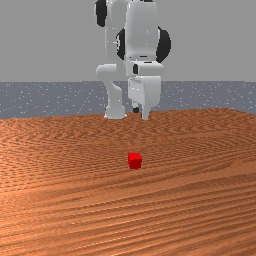
\includegraphics[width=0.118\textwidth]{media/appendix/fs_pick/f0.jpg} &
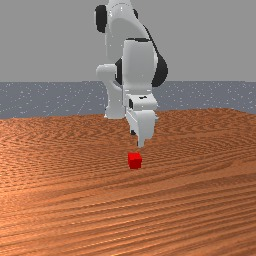
\includegraphics[width=0.118\textwidth]{media/appendix/fs_pick/f1.jpg} &
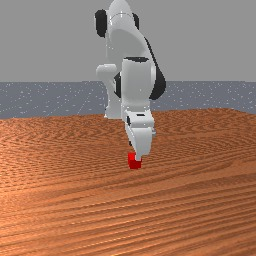
\includegraphics[width=0.118\textwidth]{media/appendix/fs_pick/f2.jpg} &
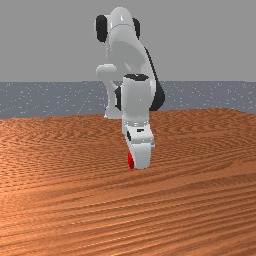
\includegraphics[width=0.118\textwidth]{media/appendix/fs_pick/f3.jpg} &
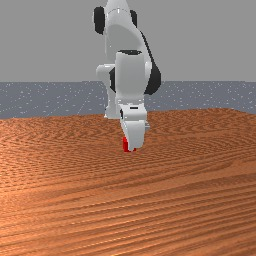
\includegraphics[width=0.118\textwidth]{media/appendix/fs_pick/f4.jpg} &
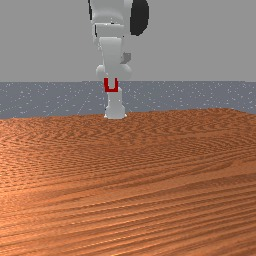
\includegraphics[width=0.118\textwidth]{media/appendix/fs_pick/f5.jpg} &
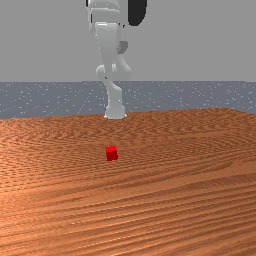
\includegraphics[width=0.118\textwidth]{media/appendix/fs_pick/f6.jpg} &
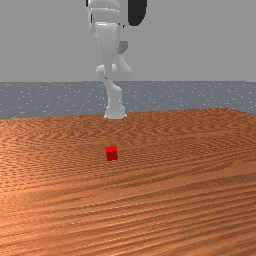
\includegraphics[width=0.118\textwidth]{media/appendix/fs_pick/f7.jpg} \\
\end{tabular}\\[2pt]
{\footnotesize Pick, grasps and lifts then releases.}\par}
\vspace{8pt}
{\centering
\setlength{\tabcolsep}{1pt}\renewcommand{\arraystretch}{0.5}
\begin{tabular}{@{}cccccccc@{}}
{\scriptsize 1} & {\scriptsize 1} & {\scriptsize 1} & {\scriptsize 2} & {\scriptsize 2} & {\scriptsize 2} & {\scriptsize 2} & {\scriptsize 4} \\

\includegraphics[width=0.118\textwidth]{media/appendix/fs_push/f0.jpg} &

\includegraphics[width=0.118\textwidth]{media/appendix/fs_push/f1.jpg} &

\includegraphics[width=0.118\textwidth]{media/appendix/fs_push/f2.jpg} &

\includegraphics[width=0.118\textwidth]{media/appendix/fs_push/f3.jpg} &

\includegraphics[width=0.118\textwidth]{media/appendix/fs_push/f4.jpg} &

\includegraphics[width=0.118\textwidth]{media/appendix/fs_push/f5.jpg} &

\includegraphics[width=0.118\textwidth]{media/appendix/fs_push/f6.jpg} &

\includegraphics[width=0.118\textwidth]{media/appendix/fs_push/f7.jpg} \\
\end{tabular}\\[2pt]
{\footnotesize Push, pushes toward the goal then stalls.}\par}
\vspace{8pt}
{\centering
\setlength{\tabcolsep}{1pt}\renewcommand{\arraystretch}{0.5}
\begin{tabular}{@{}cccccccc@{}}
{\scriptsize 1} & {\scriptsize 1} & {\scriptsize 2} & {\scriptsize 2} & {\scriptsize 3} & {\scriptsize 3} & {\scriptsize 1} & {\scriptsize 1} \\

\includegraphics[width=0.118\textwidth]{media/appendix/fs_stack/f0.jpg} &

\includegraphics[width=0.118\textwidth]{media/appendix/fs_stack/f1.jpg} &

\includegraphics[width=0.118\textwidth]{media/appendix/fs_stack/f2.jpg} &

\includegraphics[width=0.118\textwidth]{media/appendix/fs_stack/f3.jpg} &

\includegraphics[width=0.118\textwidth]{media/appendix/fs_stack/f4.jpg} &

\includegraphics[width=0.118\textwidth]{media/appendix/fs_stack/f5.jpg} &

\includegraphics[width=0.118\textwidth]{media/appendix/fs_stack/f6.jpg} &

\includegraphics[width=0.118\textwidth]{media/appendix/fs_stack/f7.jpg} \\
\end{tabular}\\[2pt]
{\footnotesize Stack, carries the cube then drops it.}\par}
\vspace{8pt}



\end{document}

%%%%%%%%%%%%%%%%%%%%%%%%%%%%%%%%%%%%%%%%%%%%%%%%%%%%%%%%%%%%%%%%%%%%%%%%%%%%%%%%
%%%%%%%%%%%%%%%%%%%%%%%%%%%%%%%%%%%%%%%%%%%%%%%%%%%%%%%%%%%%%%%%%%%%%%%%%%%%%%%%